\documentclass[12pt]{extarticle}
\usepackage[paperwidth=18in,paperheight=7.5in]{geometry}
\usepackage{amsmath}
\usepackage{hyperref}
\usepackage{multirow}
\usepackage{pdfpages}
\usepackage[utf8]{inputenc}
\title{Kaon mixing: chiral and continuum extrapolations}
\author{R Mukherjee}
\date{\today}
\begin{document}
\maketitle
\tableofcontents
\clearpage
\begin{figure}
\centering
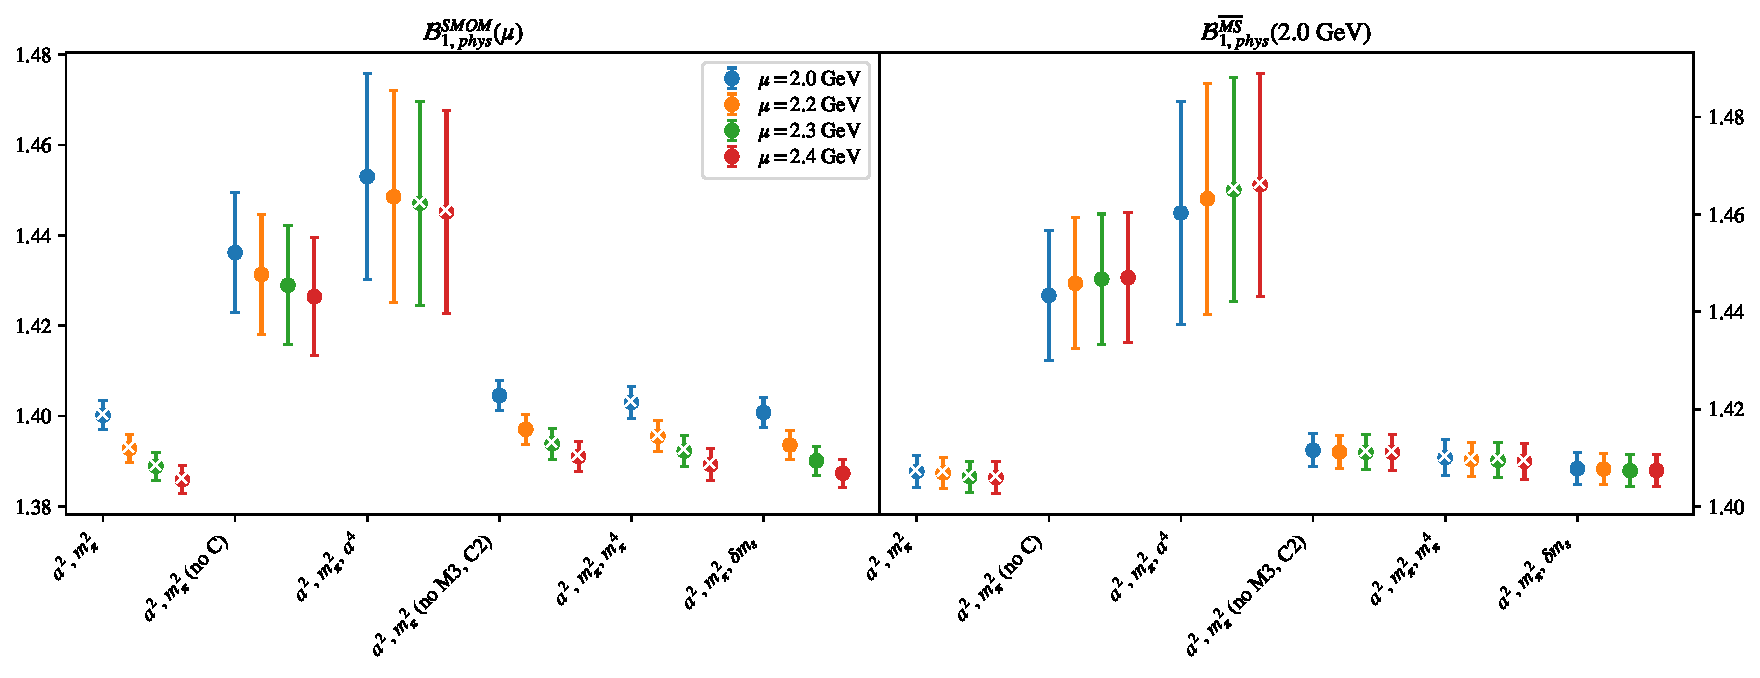
\includegraphics[page=1, width=1.1\textwidth]{VVpAA/NPR/fit_summary_bag.pdf}
\caption{$\mathcal{B}_{1}$\\(left) $\mathcal{B}_{phys}$ in RI/SMOM scheme from fit variations (fits with $p$-value $<0.05$ marked with ``$\times$"). \\(right) $\mathcal{B}_{phys}$ in $\overline{MS}$ computed using $\mathcal{B}^{\overline{MS}} = R^{\overline{MS}\leftarrow SMOM}(2.0)\sigma_{npt}(2.0,\mu) \mathcal{B}^{SMOM}(\mu)$.}
\end{figure}
\clearpage
\begin{figure}
\centering
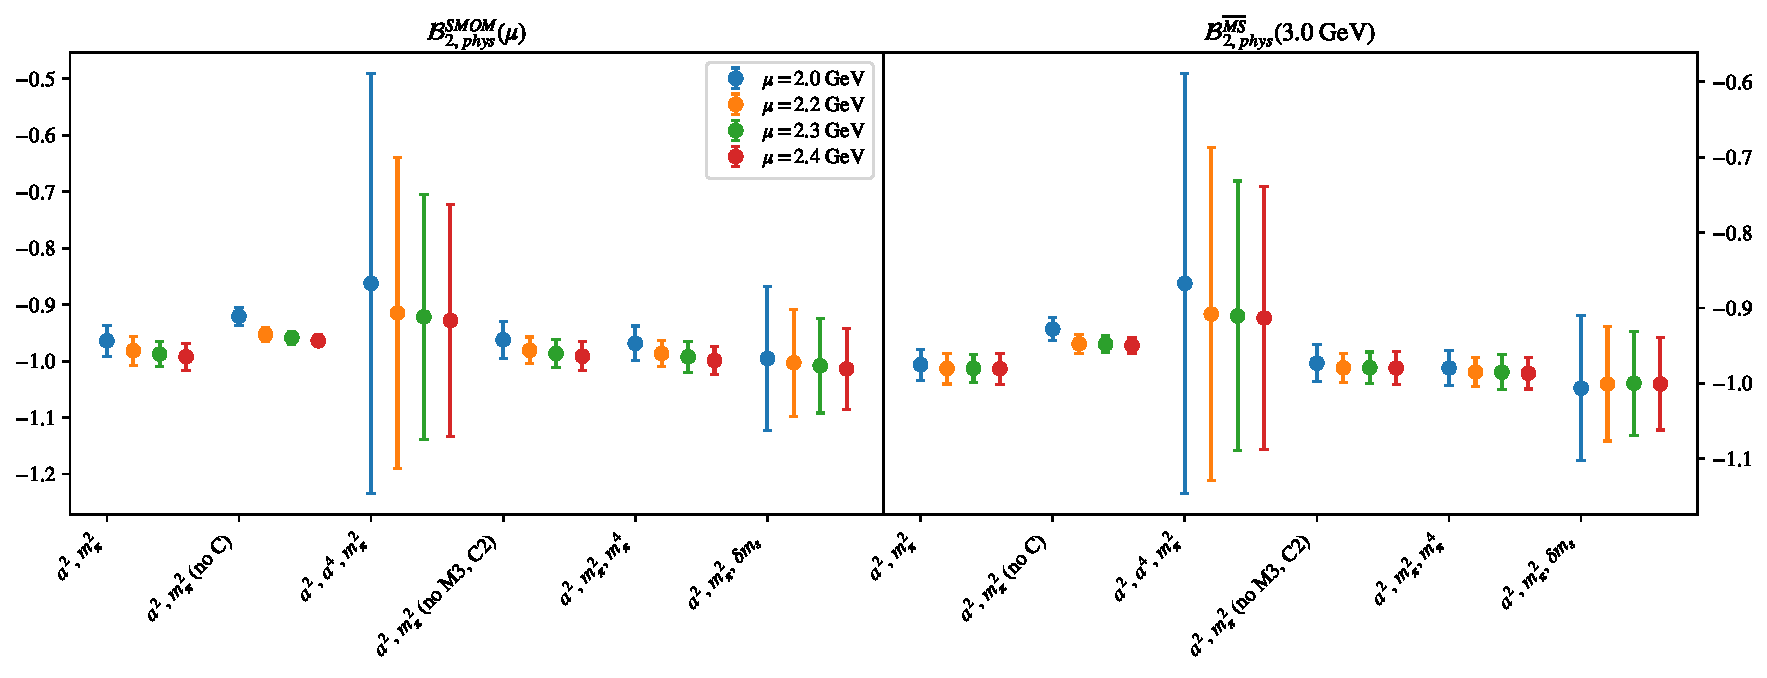
\includegraphics[page=1, width=1.1\textwidth]{VVmAA/NPR/fit_summary_bag.pdf}
\caption{$\mathcal{B}_{2}$\\(left) $\mathcal{B}_{phys}$ in RI/SMOM scheme from fit variations (fits with $p$-value $<0.05$ marked with ``$\times$"). \\(right) $\mathcal{B}_{phys}$ in $\overline{MS}$ computed using $\mathcal{B}^{\overline{MS}} = R^{\overline{MS}\leftarrow SMOM}(3.0)\sigma_{npt}(3.0,\mu) \mathcal{B}^{SMOM}(\mu)$.}
\end{figure}
\clearpage
\begin{figure}
\centering
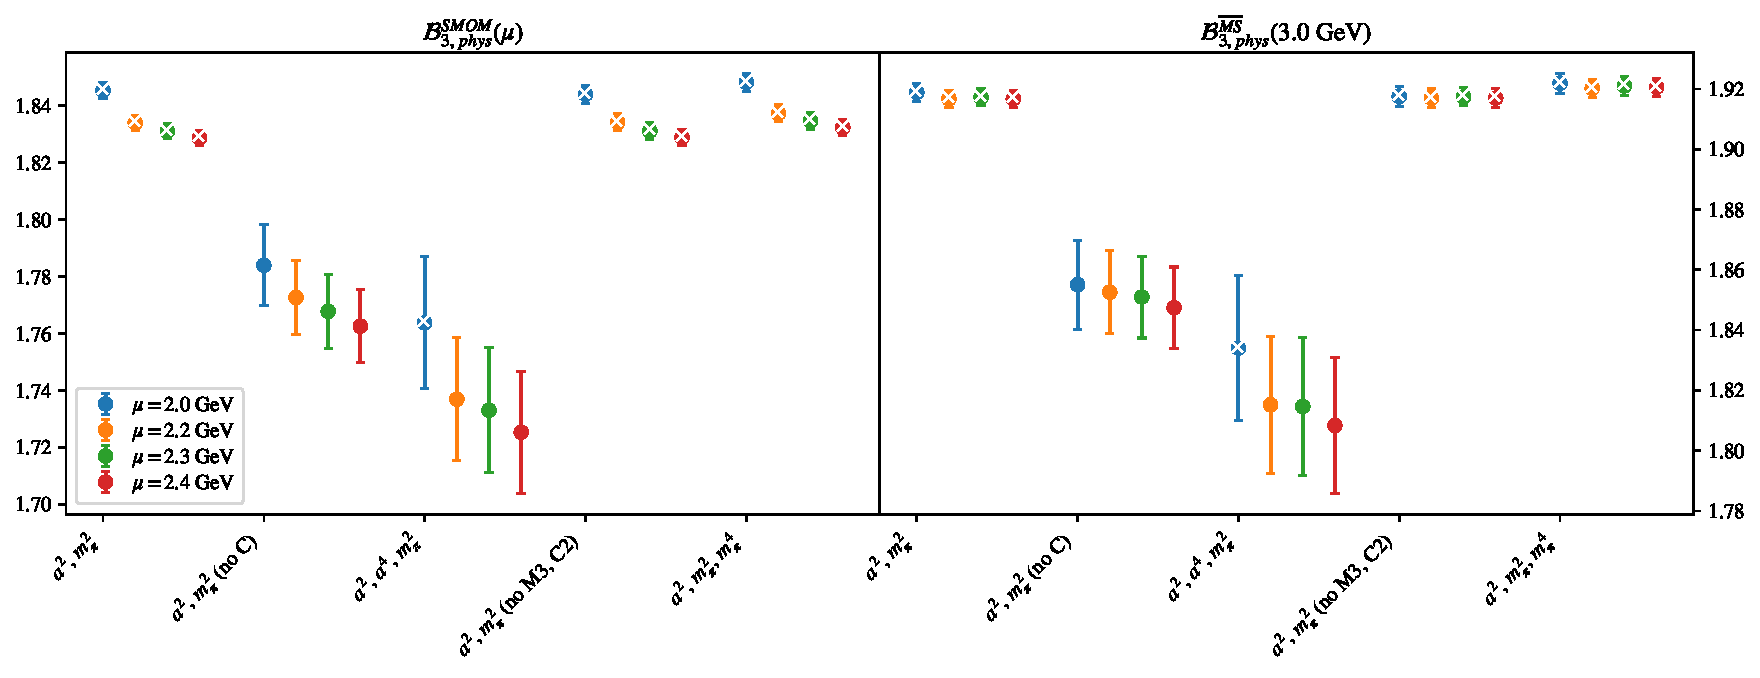
\includegraphics[page=1, width=1.1\textwidth]{SSmPP/NPR/fit_summary_bag.pdf}
\caption{$\mathcal{B}_{3}$\\(left) $\mathcal{B}_{phys}$ in RI/SMOM scheme from fit variations (fits with $p$-value $<0.05$ marked with ``$\times$"). \\(right) $\mathcal{B}_{phys}$ in $\overline{MS}$ computed using $\mathcal{B}^{\overline{MS}} = R^{\overline{MS}\leftarrow SMOM}(3.0)\sigma_{npt}(3.0,\mu) \mathcal{B}^{SMOM}(\mu)$.}
\end{figure}
\clearpage
\begin{figure}
\centering
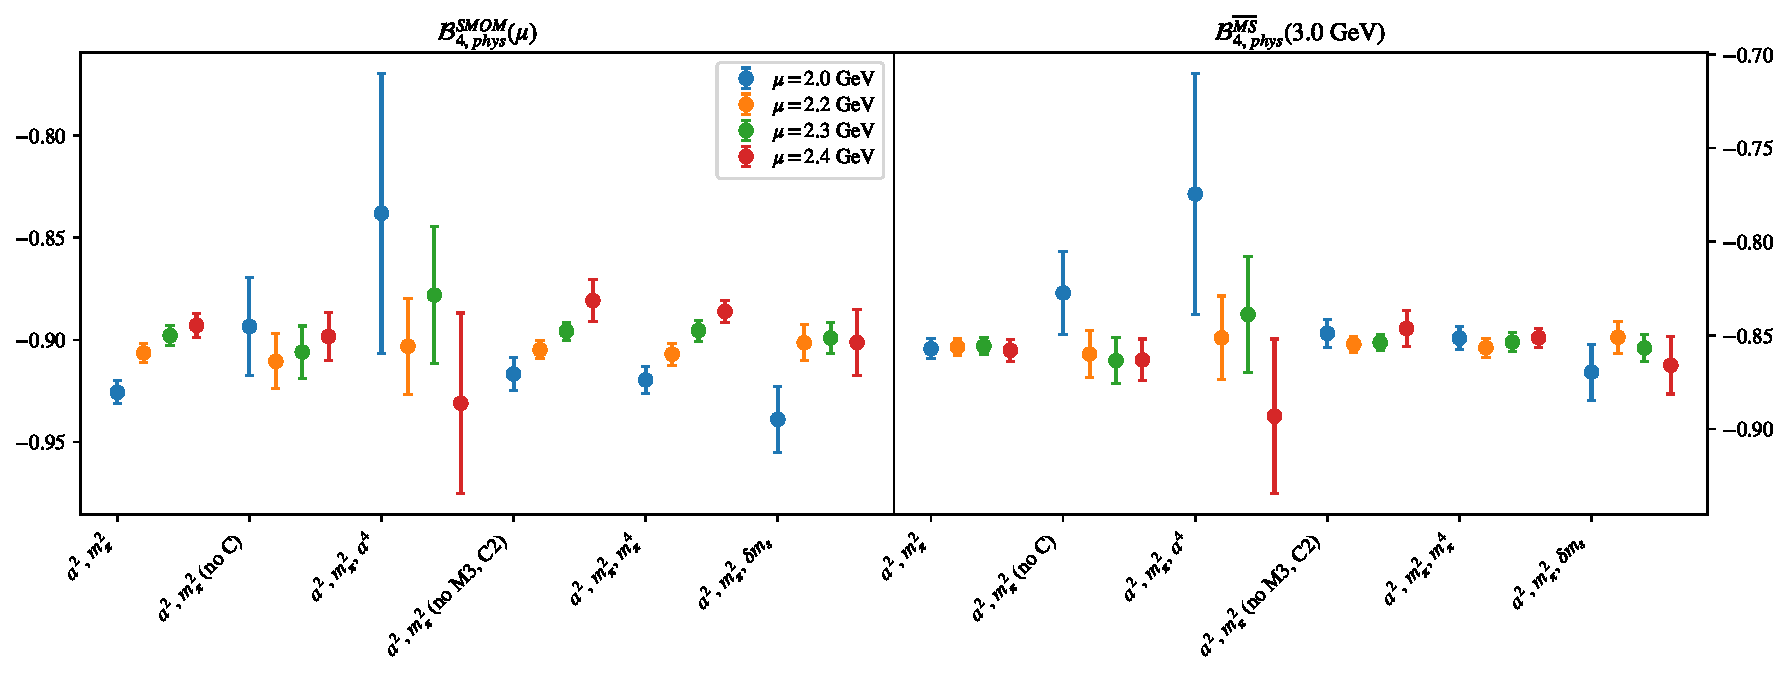
\includegraphics[page=1, width=1.1\textwidth]{SSpPP/NPR/fit_summary_bag.pdf}
\caption{$\mathcal{B}_{4}$\\(left) $\mathcal{B}_{phys}$ in RI/SMOM scheme from fit variations (fits with $p$-value $<0.05$ marked with ``$\times$"). \\(right) $\mathcal{B}_{phys}$ in $\overline{MS}$ computed using $\mathcal{B}^{\overline{MS}} = R^{\overline{MS}\leftarrow SMOM}(3.0)\sigma_{npt}(3.0,\mu) \mathcal{B}^{SMOM}(\mu)$.}
\end{figure}
\clearpage
\begin{figure}
\centering
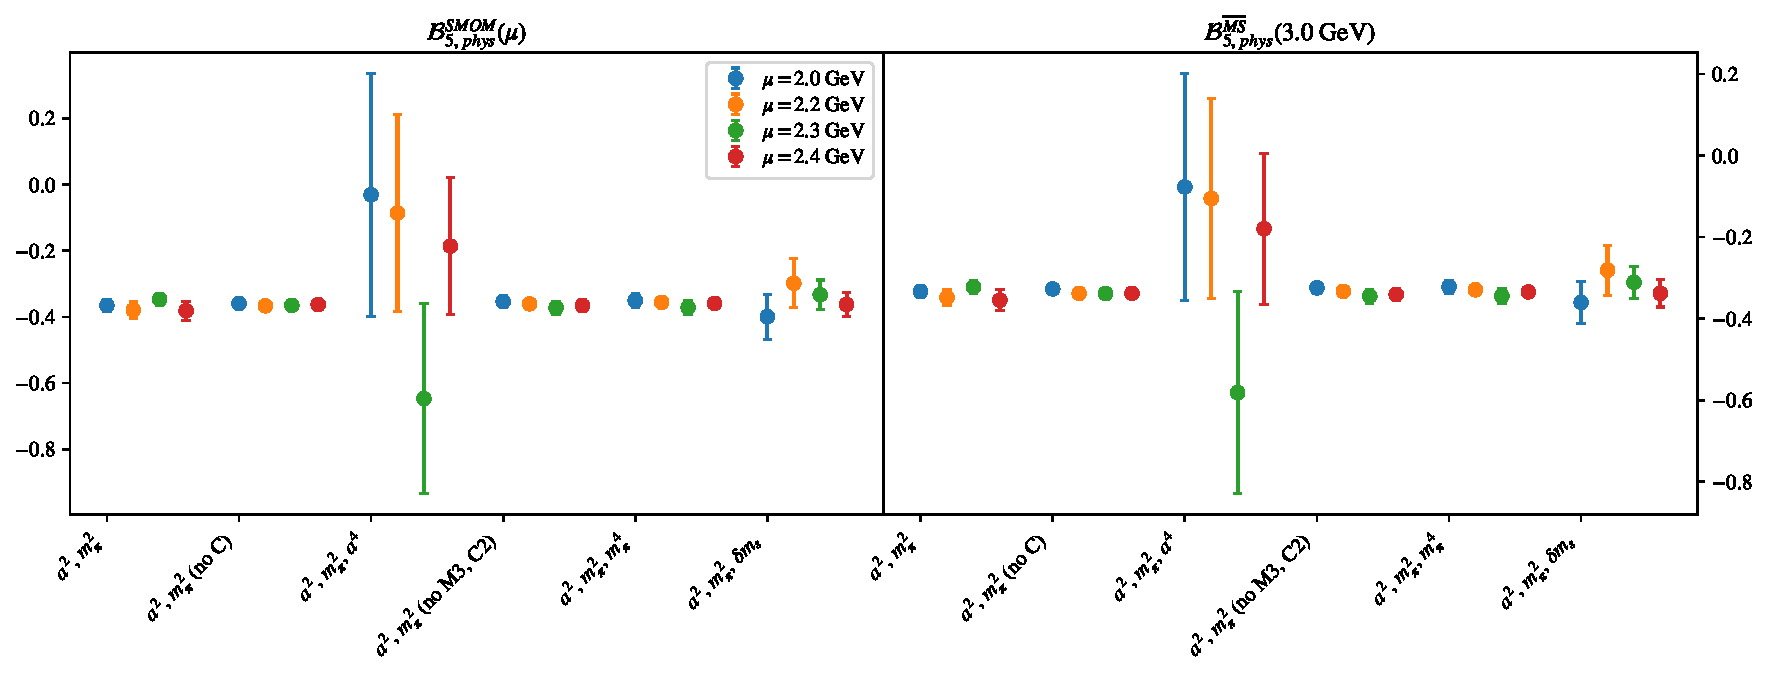
\includegraphics[page=1, width=1.1\textwidth]{TT/NPR/fit_summary_bag.pdf}
\caption{$\mathcal{B}_{5}$\\(left) $\mathcal{B}_{phys}$ in RI/SMOM scheme from fit variations (fits with $p$-value $<0.05$ marked with ``$\times$"). \\(right) $\mathcal{B}_{phys}$ in $\overline{MS}$ computed using $\mathcal{B}^{\overline{MS}} = R^{\overline{MS}\leftarrow SMOM}(3.0)\sigma_{npt}(3.0,\mu) \mathcal{B}^{SMOM}(\mu)$.}
\end{figure}
\clearpage
\section{$\mathcal{B}_1$}
\begin{table}[h!]
\begin{center}
\begin{tabular}{|c|c|c|c|c|c|c|}
\hline
$\mu$ (GeV) & $a^2$, $m_\pi^2$& $a^2$, $m_\pi^2$ (no C)& $a^2$, $a^4$, $m_\pi^2$& $a^2$, $m_\pi^2$ (no M3, C2)& $a^2$, $m_\pi^2$, $m_\pi^4$& $a^2$, $m_\pi^2$, $\delta m_s$\\
\hline
2.0& \hyperlink{VVpAA/NPR/a2m2_20.pdf.1}{\textbf{1.4038(27)}: 1.868 (0.096)} & \hyperlink{VVpAA/NPR/a2m2noC_20.pdf.1}{\textbf{1.416(12)}: 0.911 (0.402)} & \hyperlink{VVpAA/NPR/a2a4m2_20.pdf.1}{\textbf{1.421(21)}: 2.163 (0.07)} & \hyperlink{VVpAA/NPR/a2m2mcut_20.pdf.1}{\textbf{1.4089(32)}: 0.262 (0.853)} & \hyperlink{VVpAA/NPR/a2m2m4_20.pdf.1}{\textbf{1.4092(33)}: 0.693 (0.597)} & \hyperlink{VVpAA/NPR/a2m2delm_20.pdf.1}{\textbf{1.4015(32)}: 1.878 (0.111)}\\
2.2& \hyperlink{VVpAA/NPR/a2m2_22.pdf.1}{\textbf{1.3963(27)}: 2.199 (0.051)} & \hyperlink{VVpAA/NPR/a2m2noC_22.pdf.1}{\textbf{1.410(12)}: 1.151 (0.316)} & \hyperlink{VVpAA/NPR/a2a4m2_22.pdf.1}{\textbf{1.417(21)}: 2.505 (0.04)} & \hyperlink{VVpAA/NPR/a2m2mcut_22.pdf.1}{\textbf{1.4018(32)}: 0.357 (0.784)} & \hyperlink{VVpAA/NPR/a2m2m4_22.pdf.1}{\textbf{1.4020(33)}: 0.912 (0.456)} & \hyperlink{VVpAA/NPR/a2m2delm_22.pdf.1}{\textbf{1.3937(32)}: 2.13 (0.074)}\\
2.3& \hyperlink{VVpAA/NPR/a2m2_23.pdf.1}{\textbf{1.3931(27)}: 2.287 (0.043)} & \hyperlink{VVpAA/NPR/a2m2noC_23.pdf.1}{\textbf{1.408(12)}: 1.196 (0.303)} & \hyperlink{VVpAA/NPR/a2a4m2_23.pdf.1}{\textbf{1.415(21)}: 2.583 (0.035)} & \hyperlink{VVpAA/NPR/a2m2mcut_23.pdf.1}{\textbf{1.3986(32)}: 0.407 (0.748)} & \hyperlink{VVpAA/NPR/a2m2m4_23.pdf.1}{\textbf{1.3988(33)}: 0.98 (0.417)} & \hyperlink{VVpAA/NPR/a2m2delm_23.pdf.1}{\textbf{1.3903(32)}: 2.173 (0.069)}\\
2.4& \hyperlink{VVpAA/NPR/a2m2_24.pdf.1}{\textbf{1.3902(26)}: 2.336 (0.039)} & \hyperlink{VVpAA/NPR/a2m2noC_24.pdf.1}{\textbf{1.405(12)}: 1.221 (0.295)} & \hyperlink{VVpAA/NPR/a2a4m2_24.pdf.1}{\textbf{1.412(21)}: 2.644 (0.032)} & \hyperlink{VVpAA/NPR/a2m2mcut_24.pdf.1}{\textbf{1.3958(32)}: 0.408 (0.747)} & \hyperlink{VVpAA/NPR/a2m2m4_24.pdf.1}{\textbf{1.3960(33)}: 0.996 (0.408)} & \hyperlink{VVpAA/NPR/a2m2delm_24.pdf.1}{\textbf{1.3874(32)}: 2.22 (0.064)}\\
\hline
\end{tabular}
\caption{Physical point value from chiral and continuum extrapolation at renormalisation scale $\mu$. Entries are \textbf{value(error)}: $\chi^2/\text{DOF}$ ($p$-value).}
\end{center}
\end{table}
\begin{table}[h!]
\begin{center}
\begin{tabular}{|c c|c|c|c|c|c|c|}
\hline
$\mu$ (GeV) &  & $a^2$, $m_\pi^2$& $a^2$, $m_\pi^2$ (no C)& $a^2$, $a^4$, $m_\pi^2$& $a^2$, $m_\pi^2$ (no M3, C2)& $a^2$, $m_\pi^2$, $m_\pi^4$& $a^2$, $m_\pi^2$, $\delta m_s$\\
\hline
\multirow{2}{0.5in}{2.0} & $\alpha$ & 0.0936(70)& 0.047(53)& -0.022& 0.0814(82)& 0.0811(82)& 0.0987(80)\\
 & $\beta$ & 0.00261(14)& 0.00224(27)& 0.00263(15)& 0.00188(29)& 0.00032(90)& 0.00269(16)\\
\hline
\multirow{2}{0.5in}{2.2} & $\alpha$ & 0.0978(70)& 0.042(53)& -0.04& 0.0848(83)& 0.0847(82)& 0.1039(80)\\
 & $\beta$ & 0.00261(14)& 0.00221(27)& 0.00265(15)& 0.00183(28)& 0.00019(90)& 0.00271(16)\\
\hline
\multirow{2}{0.5in}{2.3} & $\alpha$ & 0.0993(70)& 0.039(53)& -0.047& 0.0860(83)& 0.0860(82)& 0.1057(80)\\
 & $\beta$ & 0.00262(15)& 0.00220(27)& 0.00265(15)& 0.00183(28)& 0.00018(90)& 0.00272(16)\\
\hline
\multirow{2}{0.5in}{2.4} & $\alpha$ & 0.1000(70)& 0.040(53)& -0.046& 0.0865(83)& 0.0865(82)& 0.1064(80)\\
 & $\beta$ & 0.00263(15)& 0.00221(27)& 0.00267(15)& 0.00184(28)& 0.00016(90)& 0.00273(16)\\
\hline
\end{tabular}
\caption{Fit values of coefficients in $Q = Q_{phys} + \mathbf{\alpha} a^2 + \mathbf{\beta}\left(\frac{m_\pi^2}{f_\pi^2}-\frac{m_{\pi,PDG}^2}{f_\pi^2}\right) + \ldots$.}
\end{center}
\end{table}
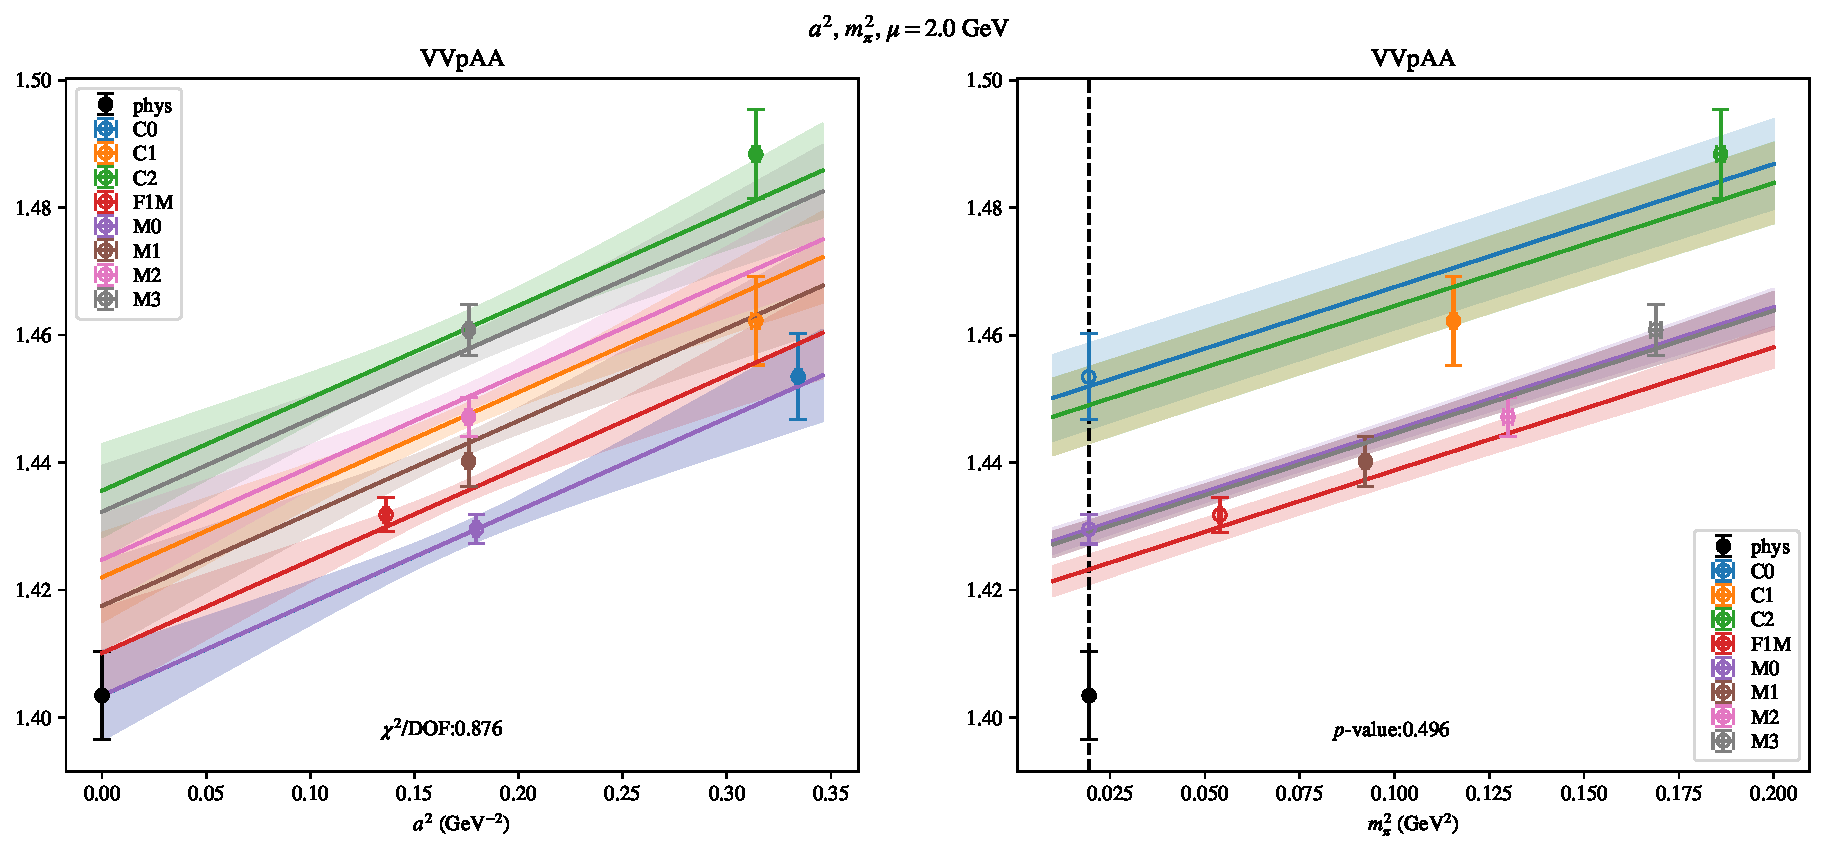
\includepdf[link, pages=-]{VVpAA/NPR/a2m2_20.pdf}
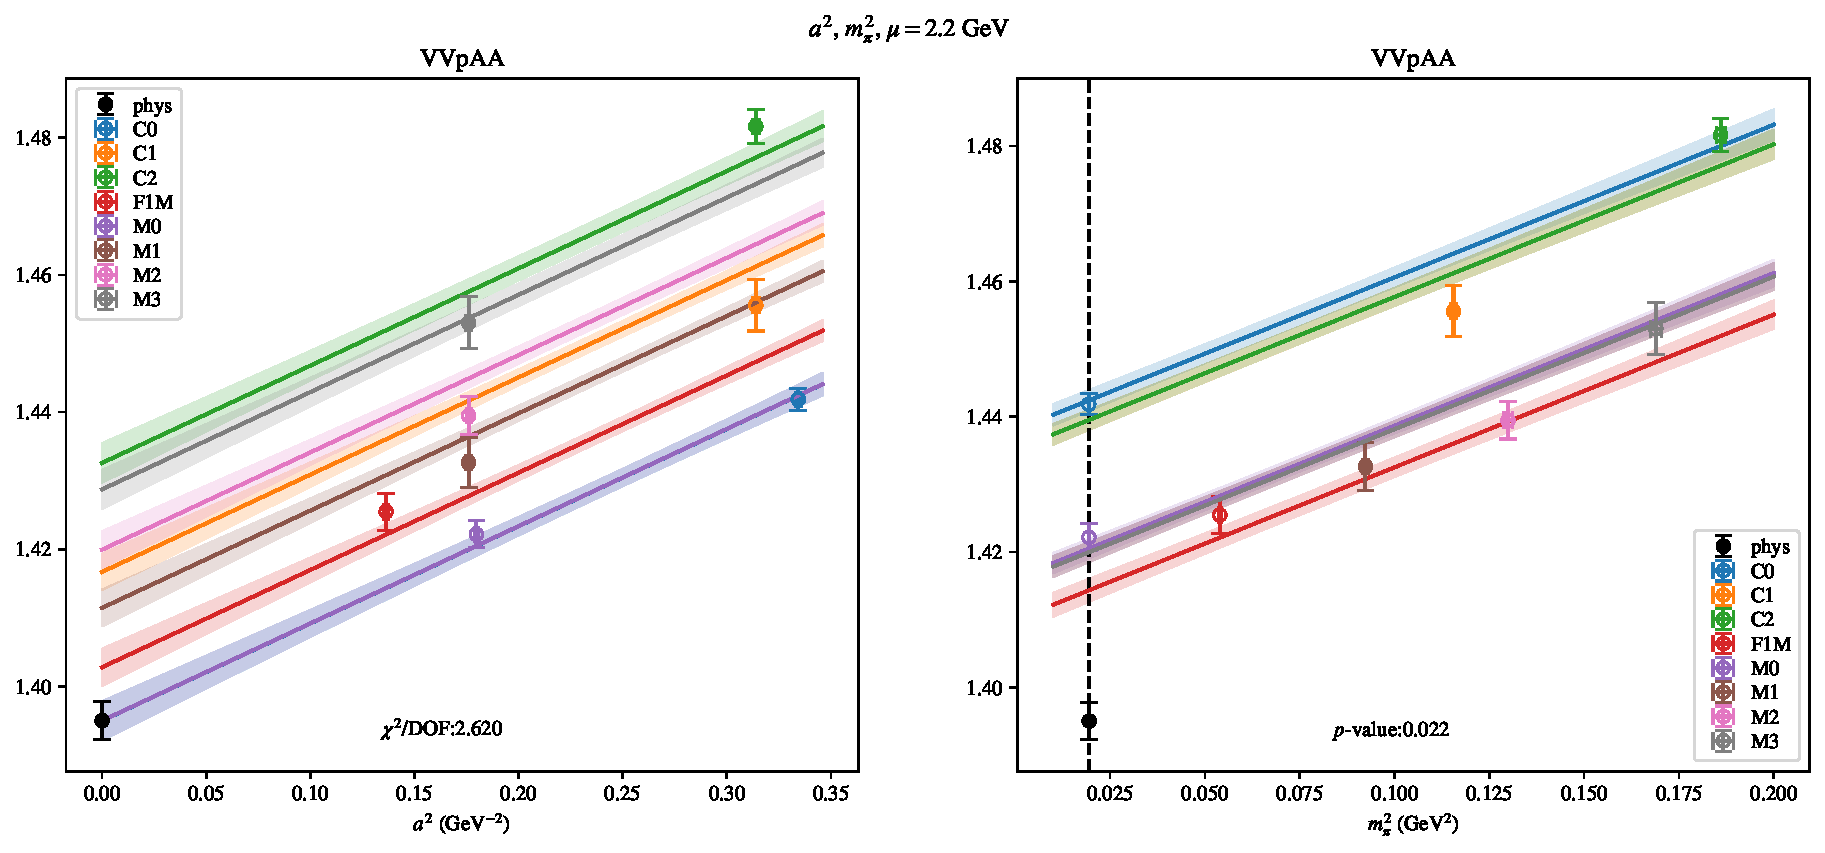
\includepdf[link, pages=-]{VVpAA/NPR/a2m2_22.pdf}
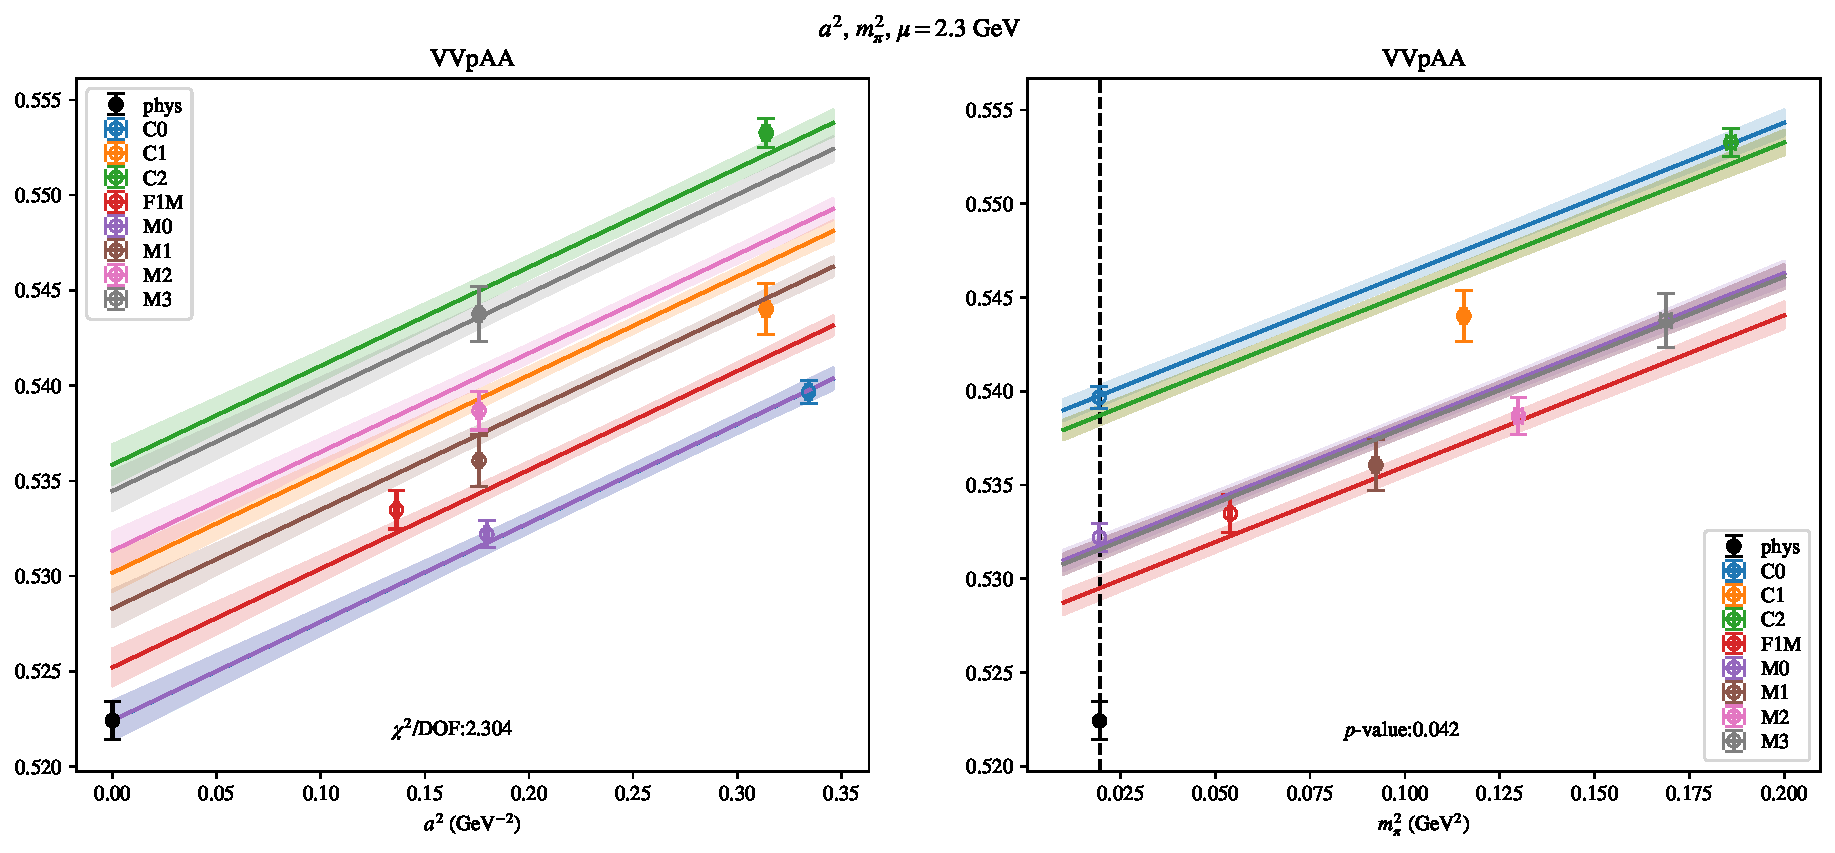
\includepdf[link, pages=-]{VVpAA/NPR/a2m2_23.pdf}
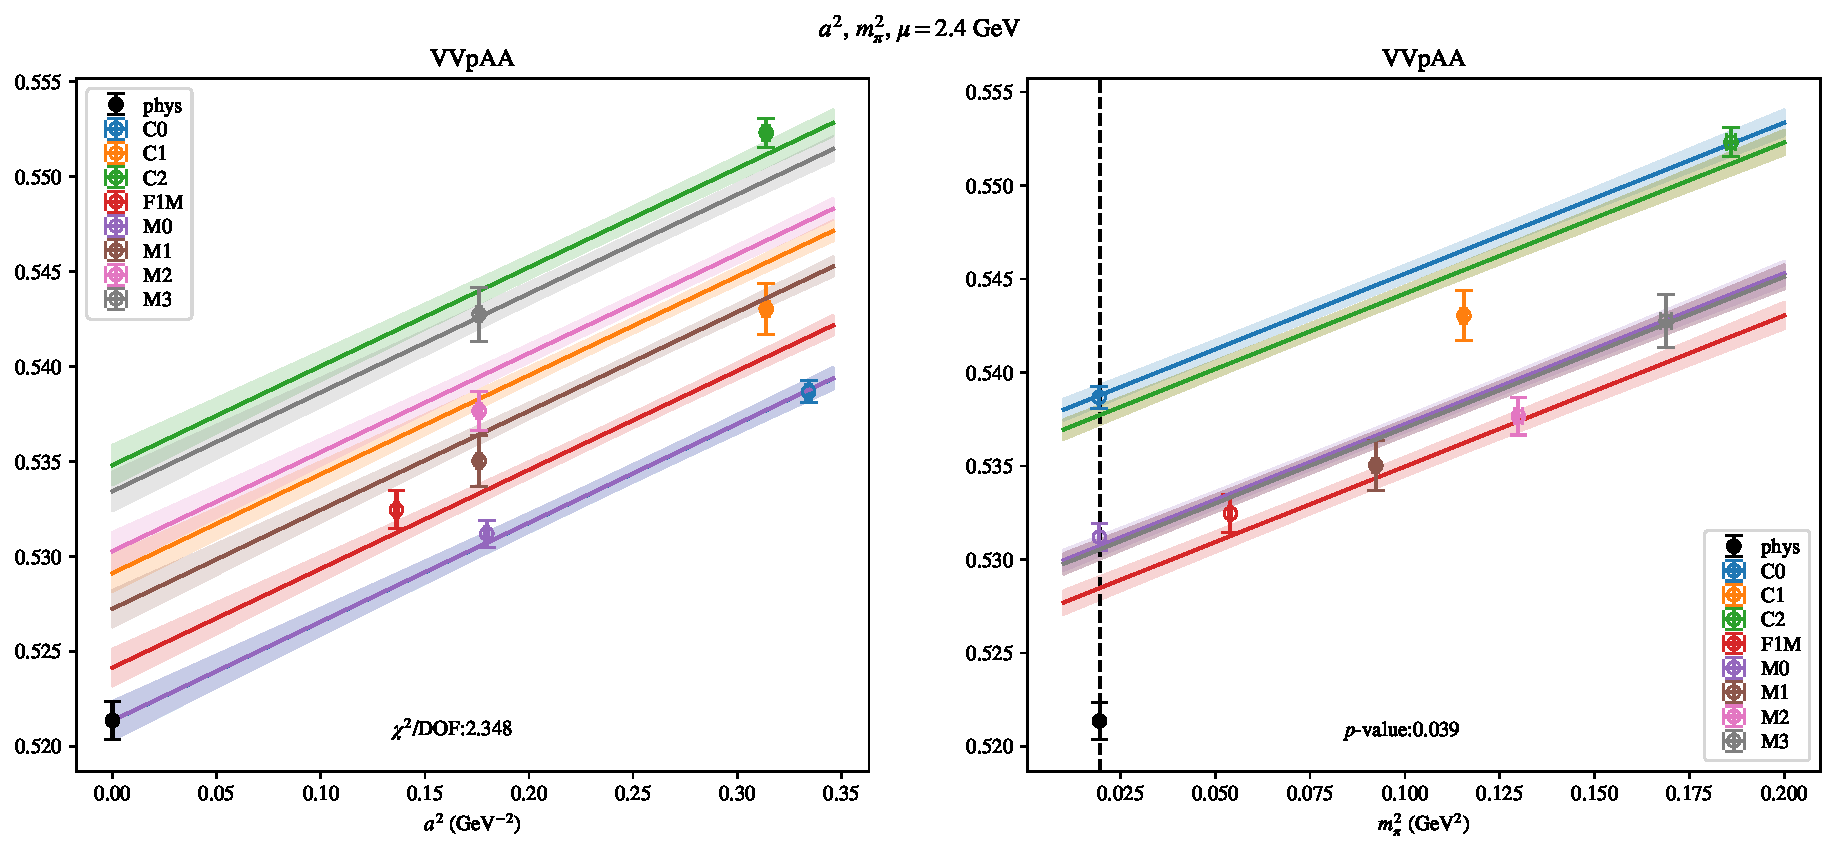
\includepdf[link, pages=-]{VVpAA/NPR/a2m2_24.pdf}
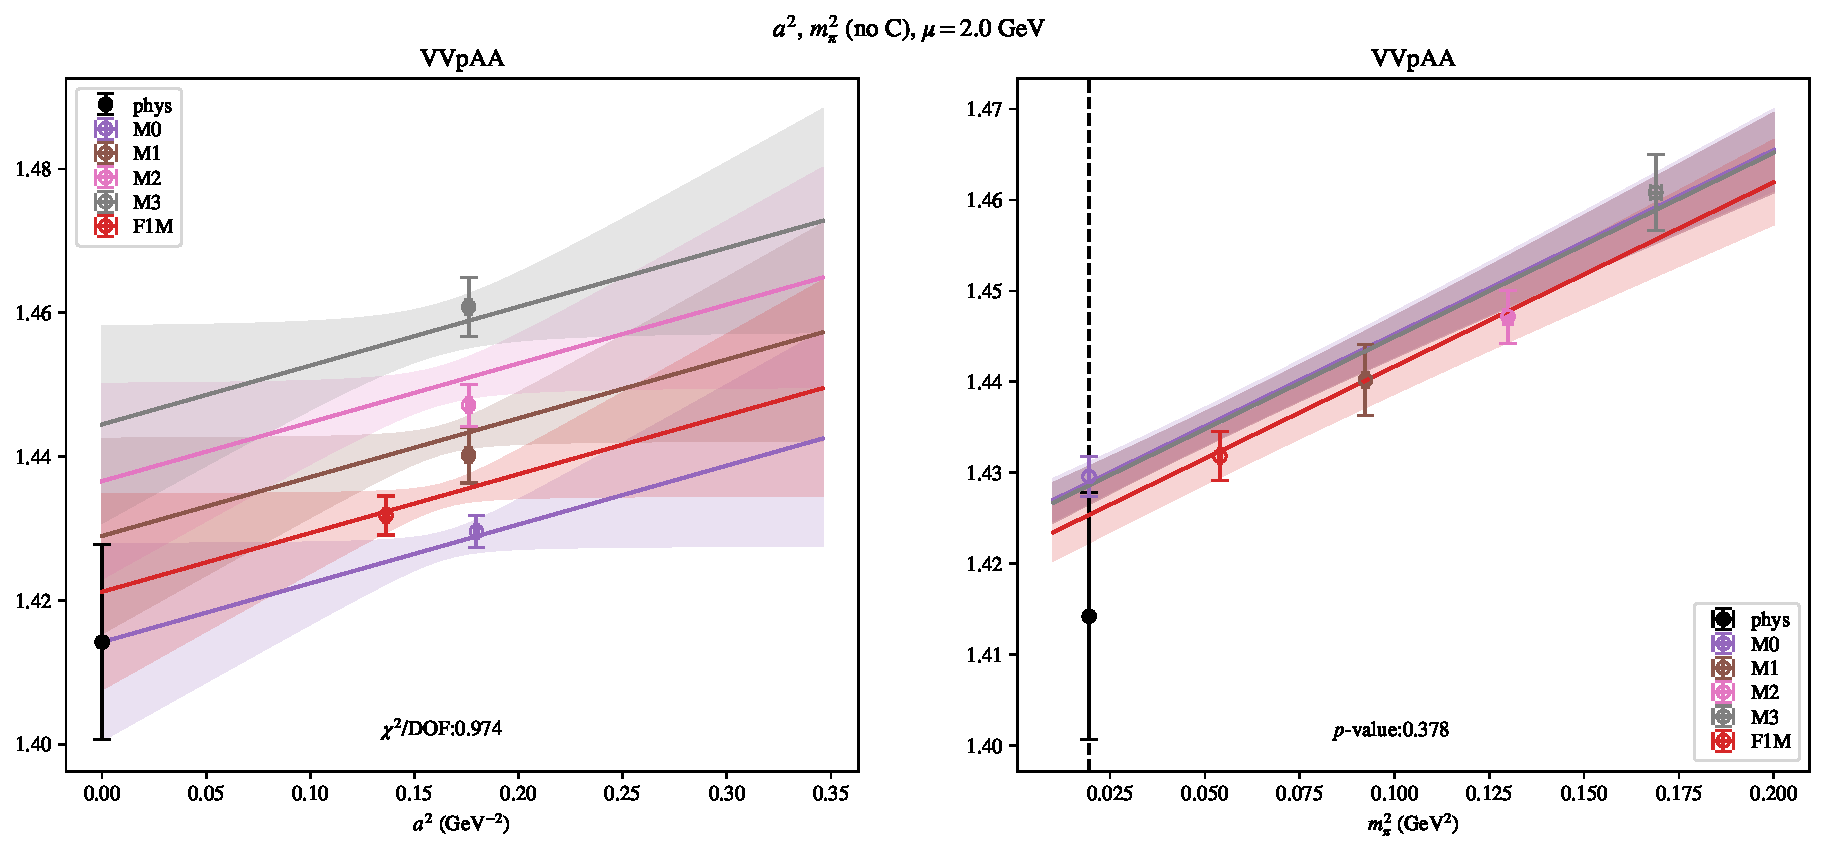
\includepdf[link, pages=-]{VVpAA/NPR/a2m2noC_20.pdf}
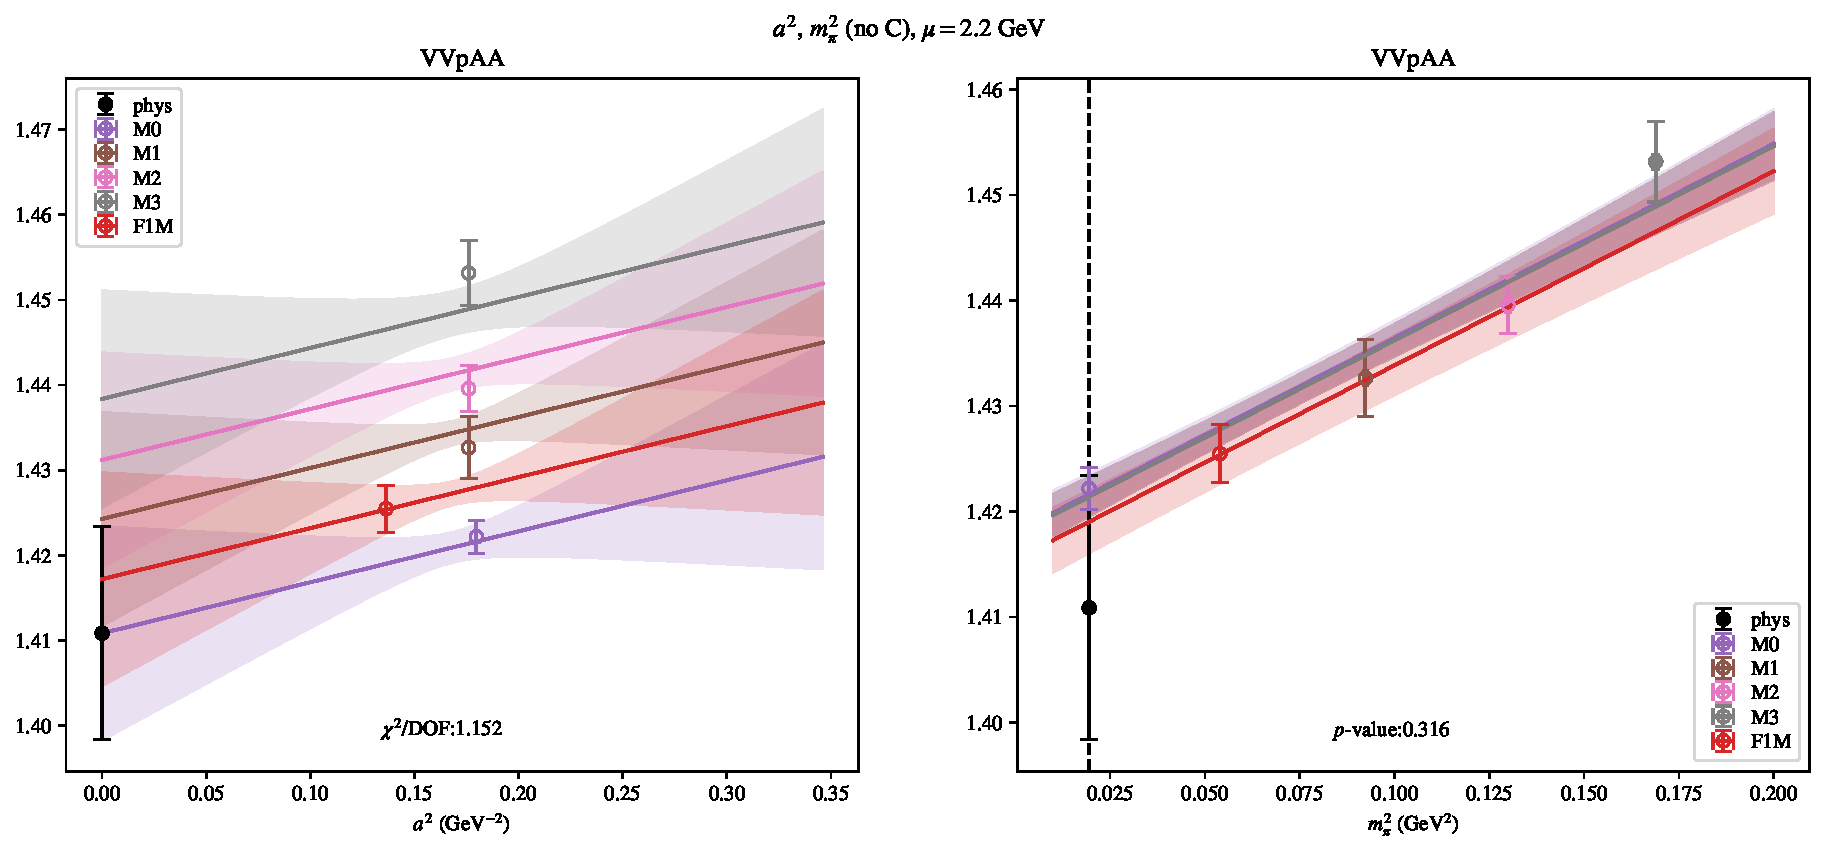
\includepdf[link, pages=-]{VVpAA/NPR/a2m2noC_22.pdf}
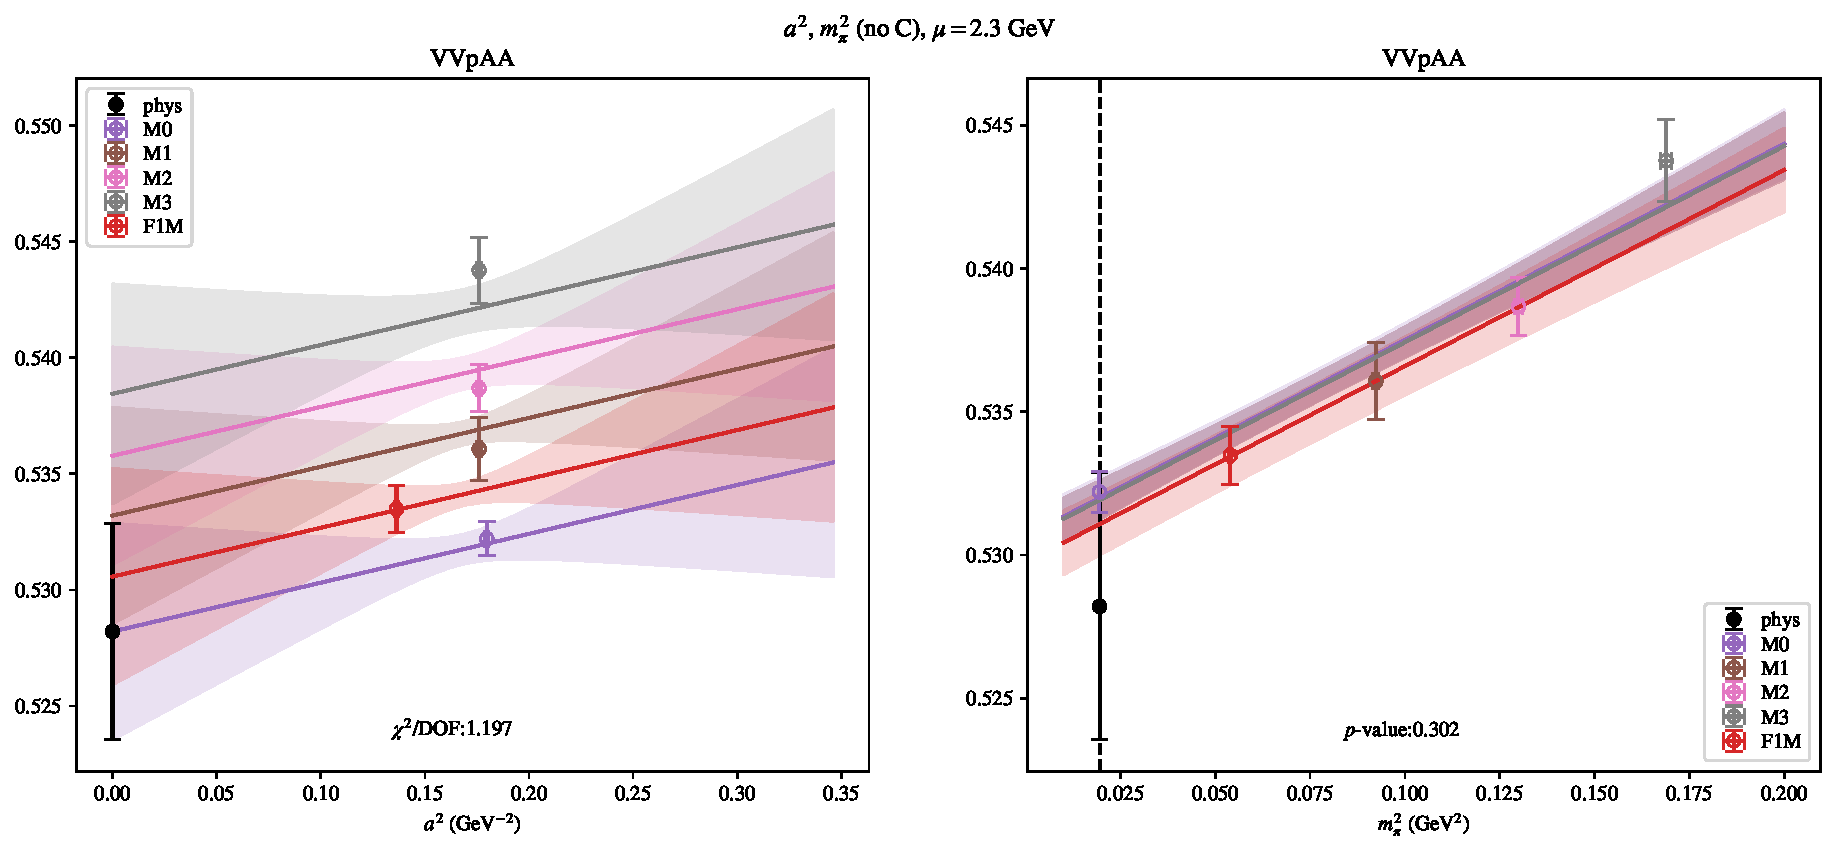
\includepdf[link, pages=-]{VVpAA/NPR/a2m2noC_23.pdf}
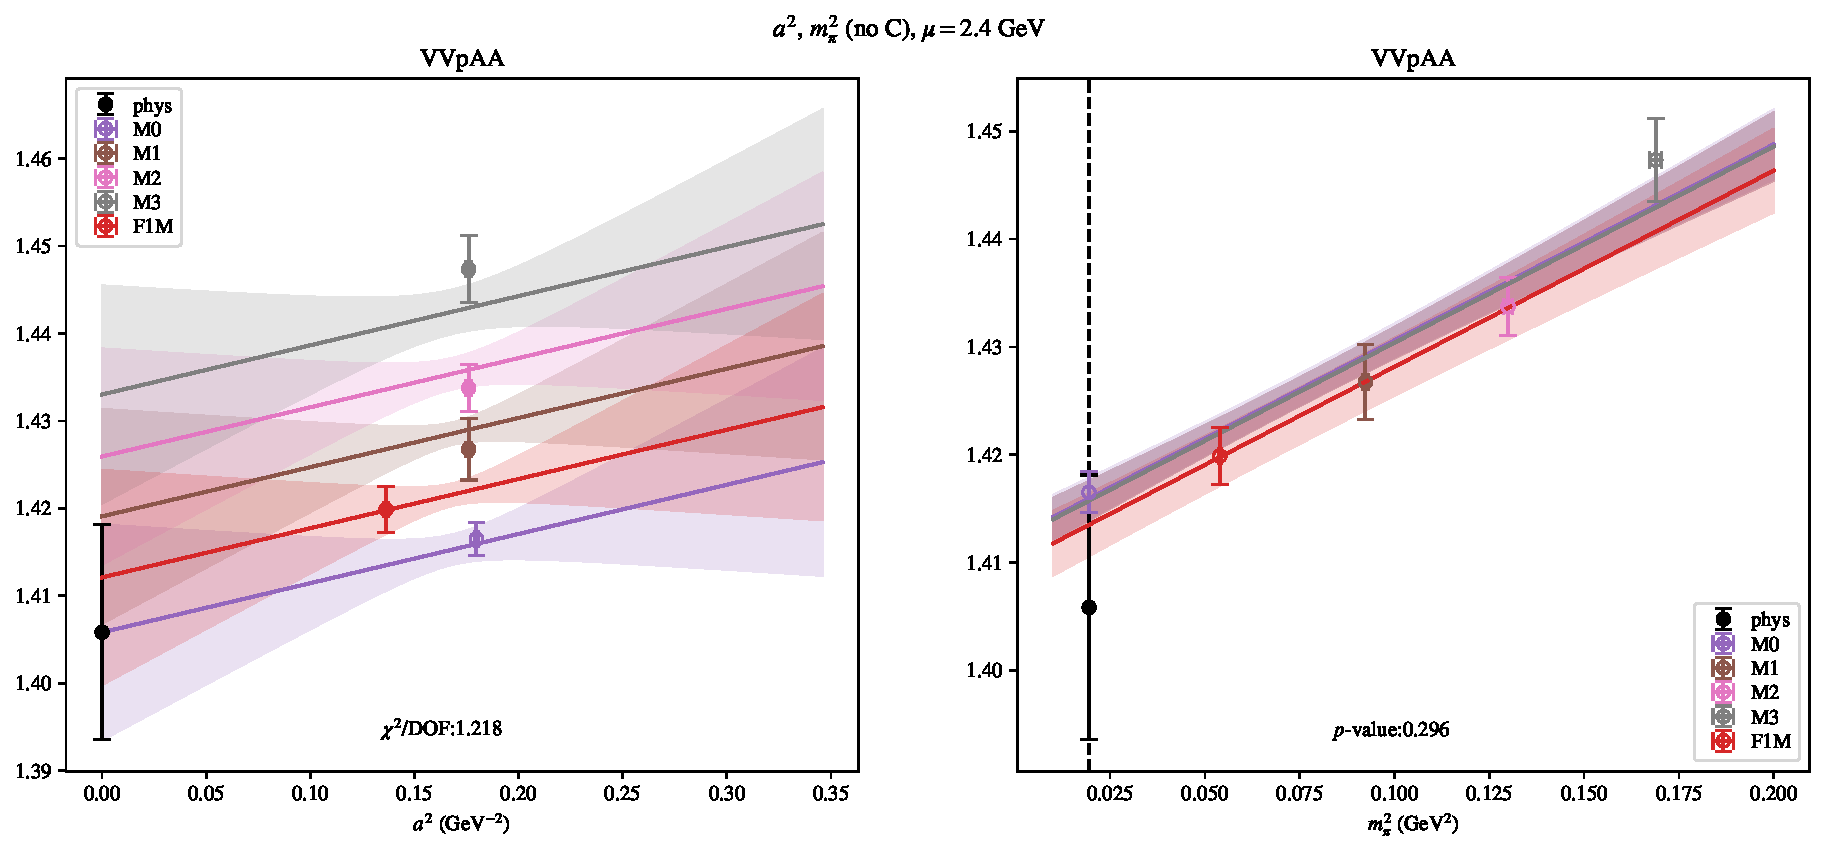
\includepdf[link, pages=-]{VVpAA/NPR/a2m2noC_24.pdf}
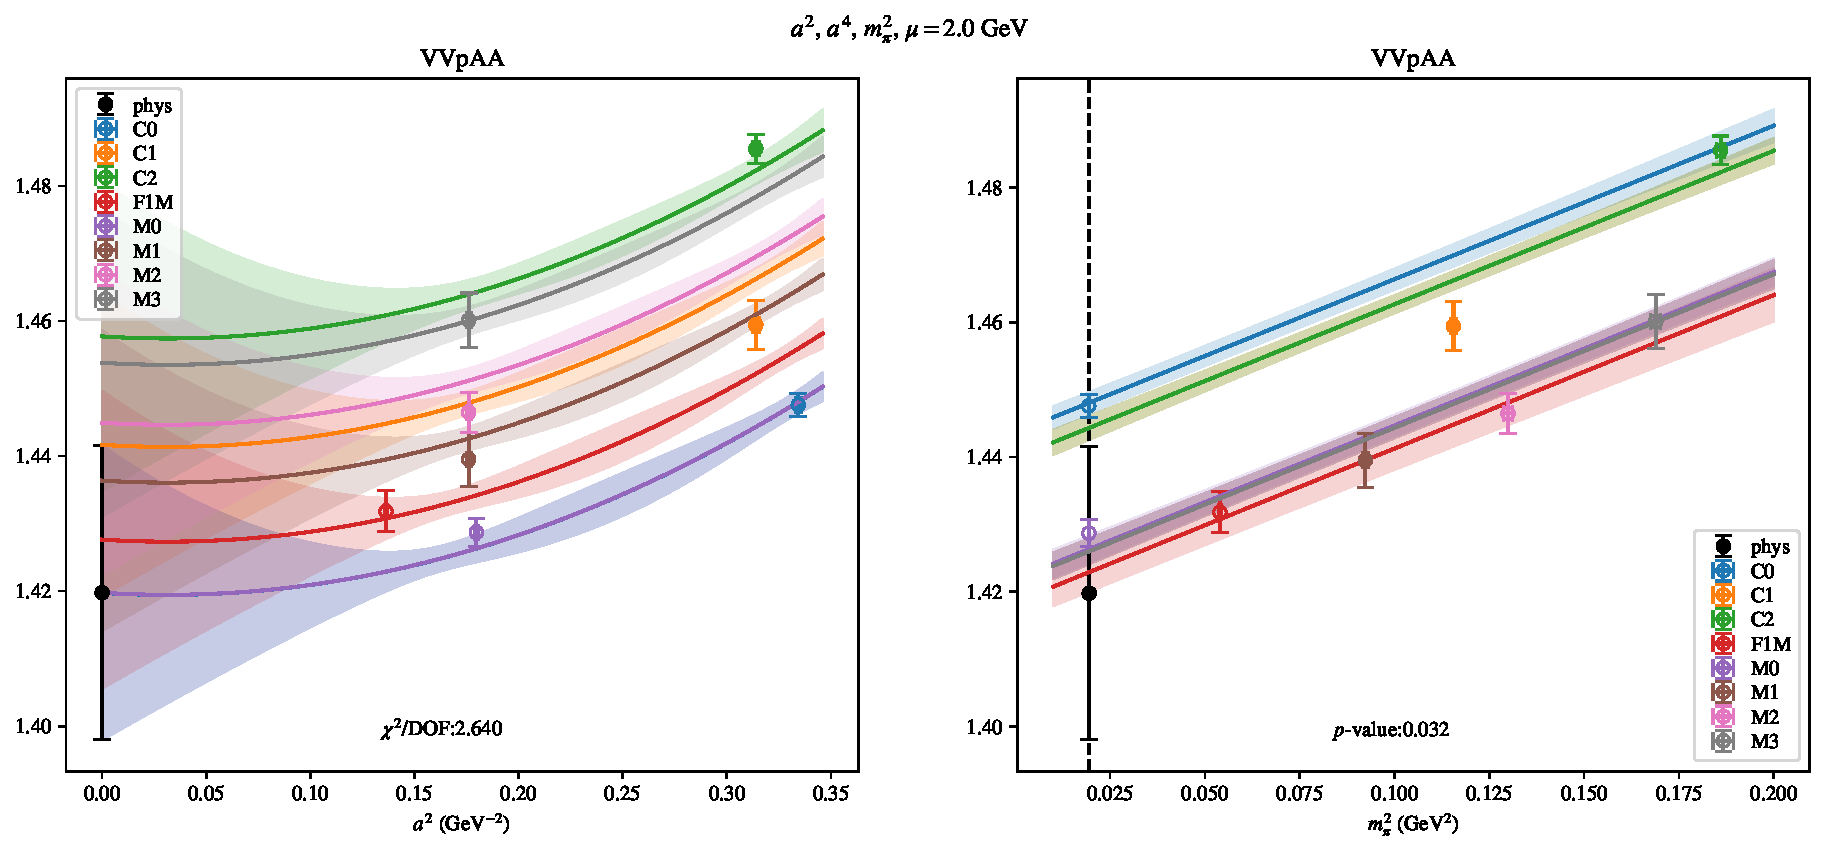
\includepdf[link, pages=-]{VVpAA/NPR/a2a4m2_20.pdf}
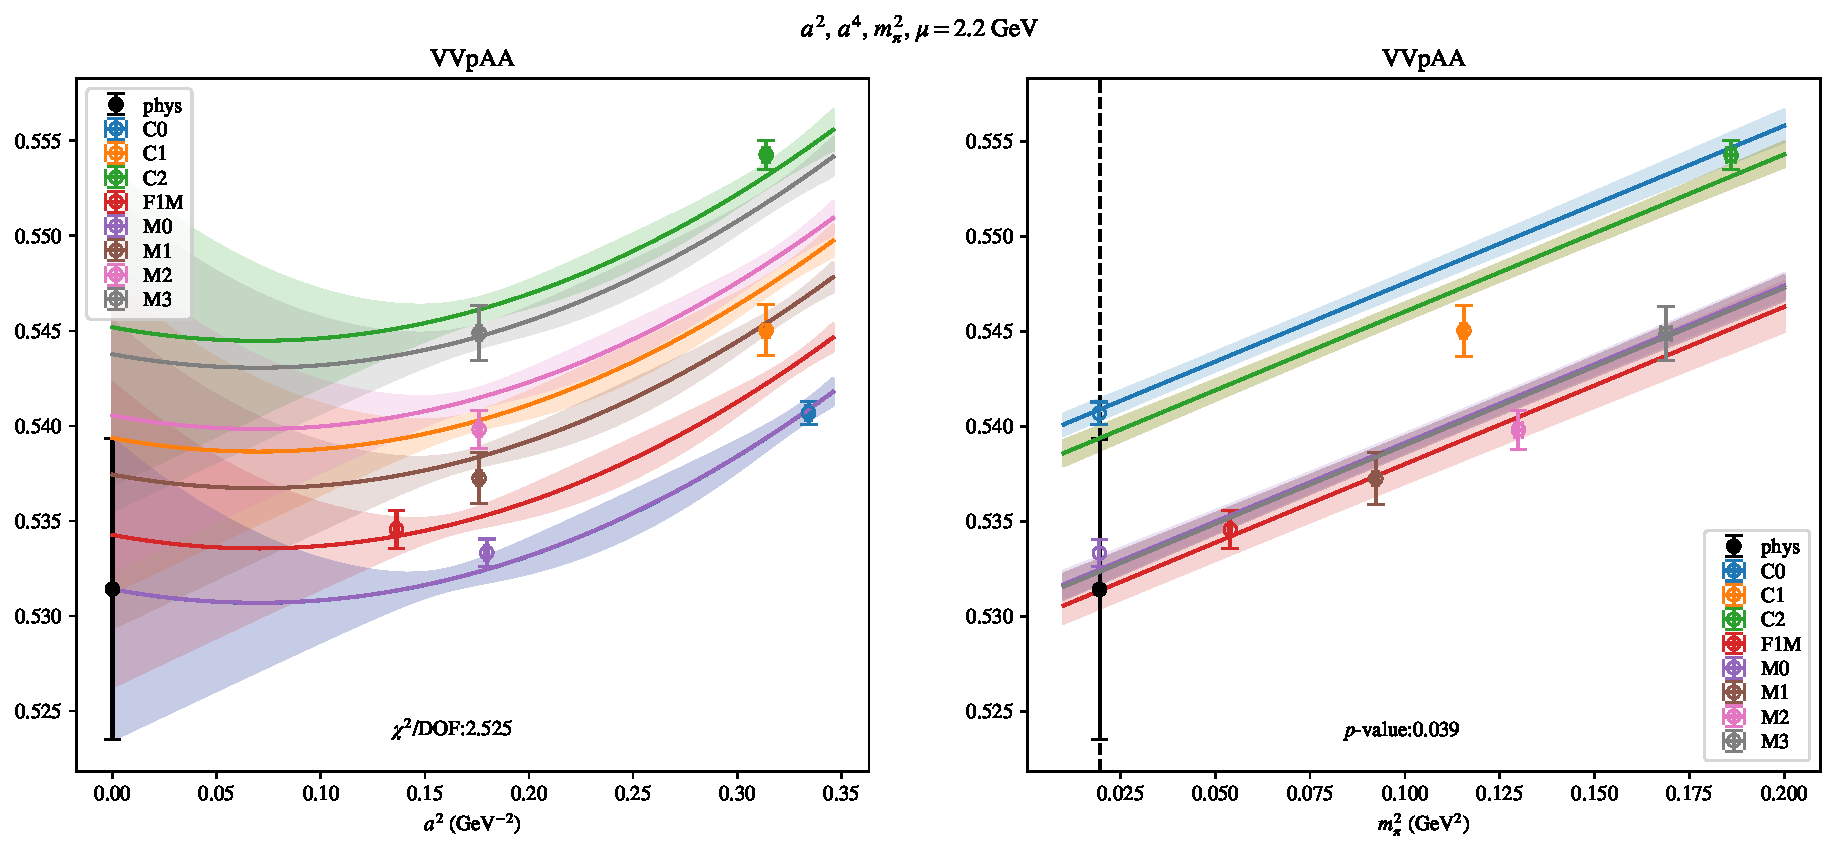
\includepdf[link, pages=-]{VVpAA/NPR/a2a4m2_22.pdf}
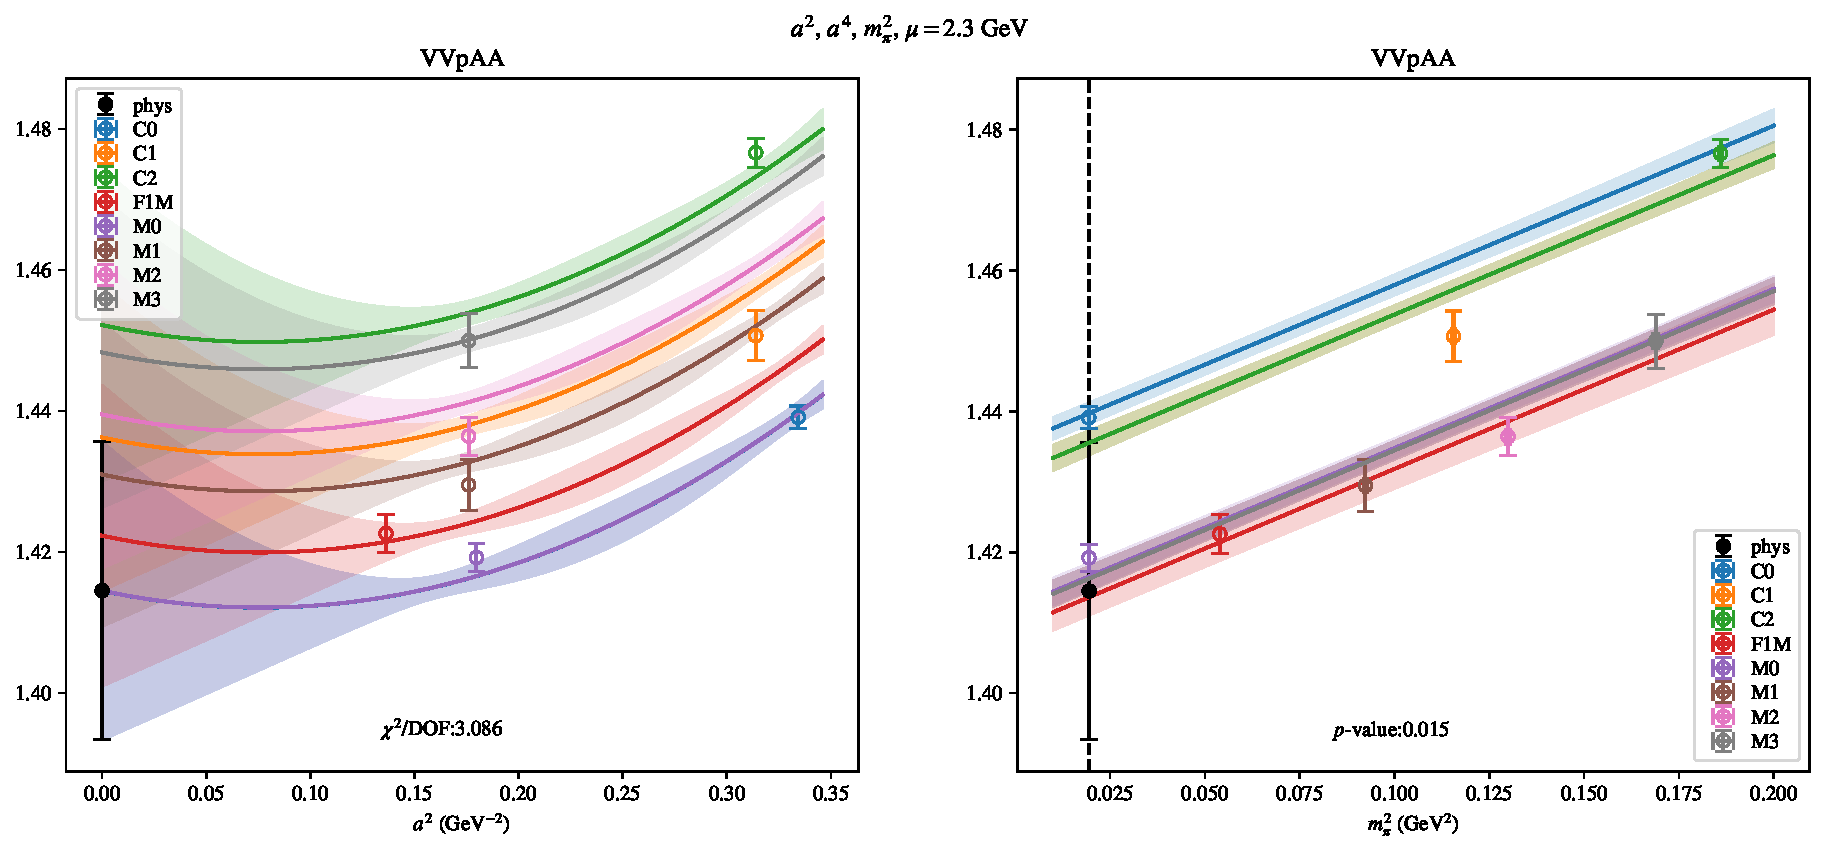
\includepdf[link, pages=-]{VVpAA/NPR/a2a4m2_23.pdf}
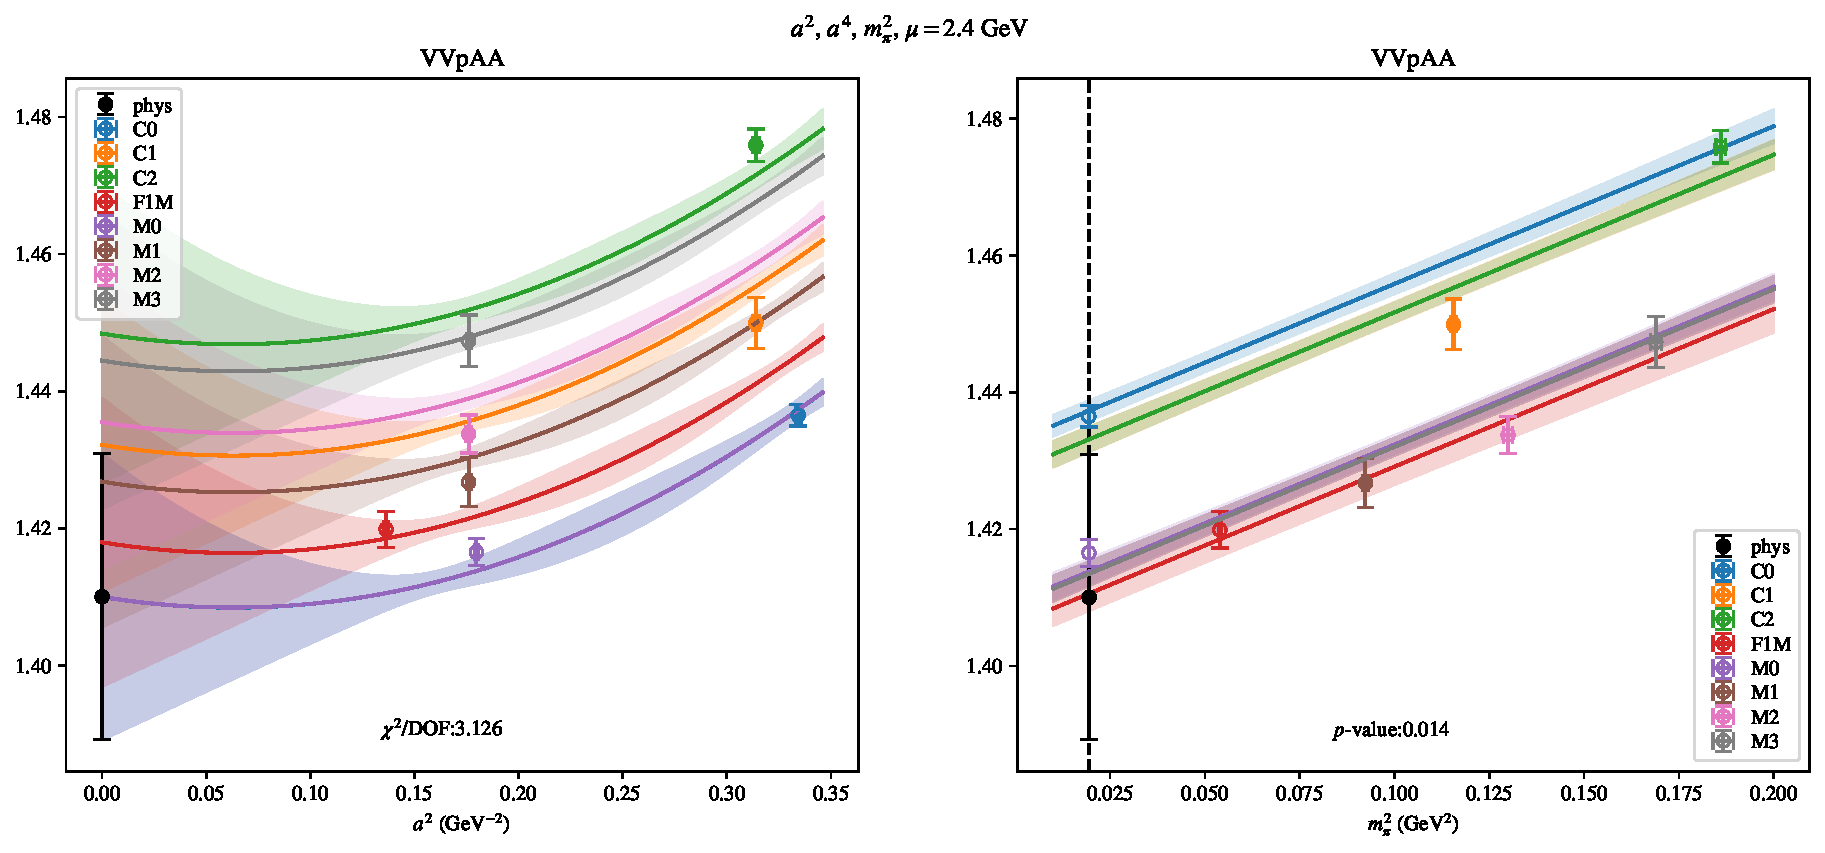
\includepdf[link, pages=-]{VVpAA/NPR/a2a4m2_24.pdf}
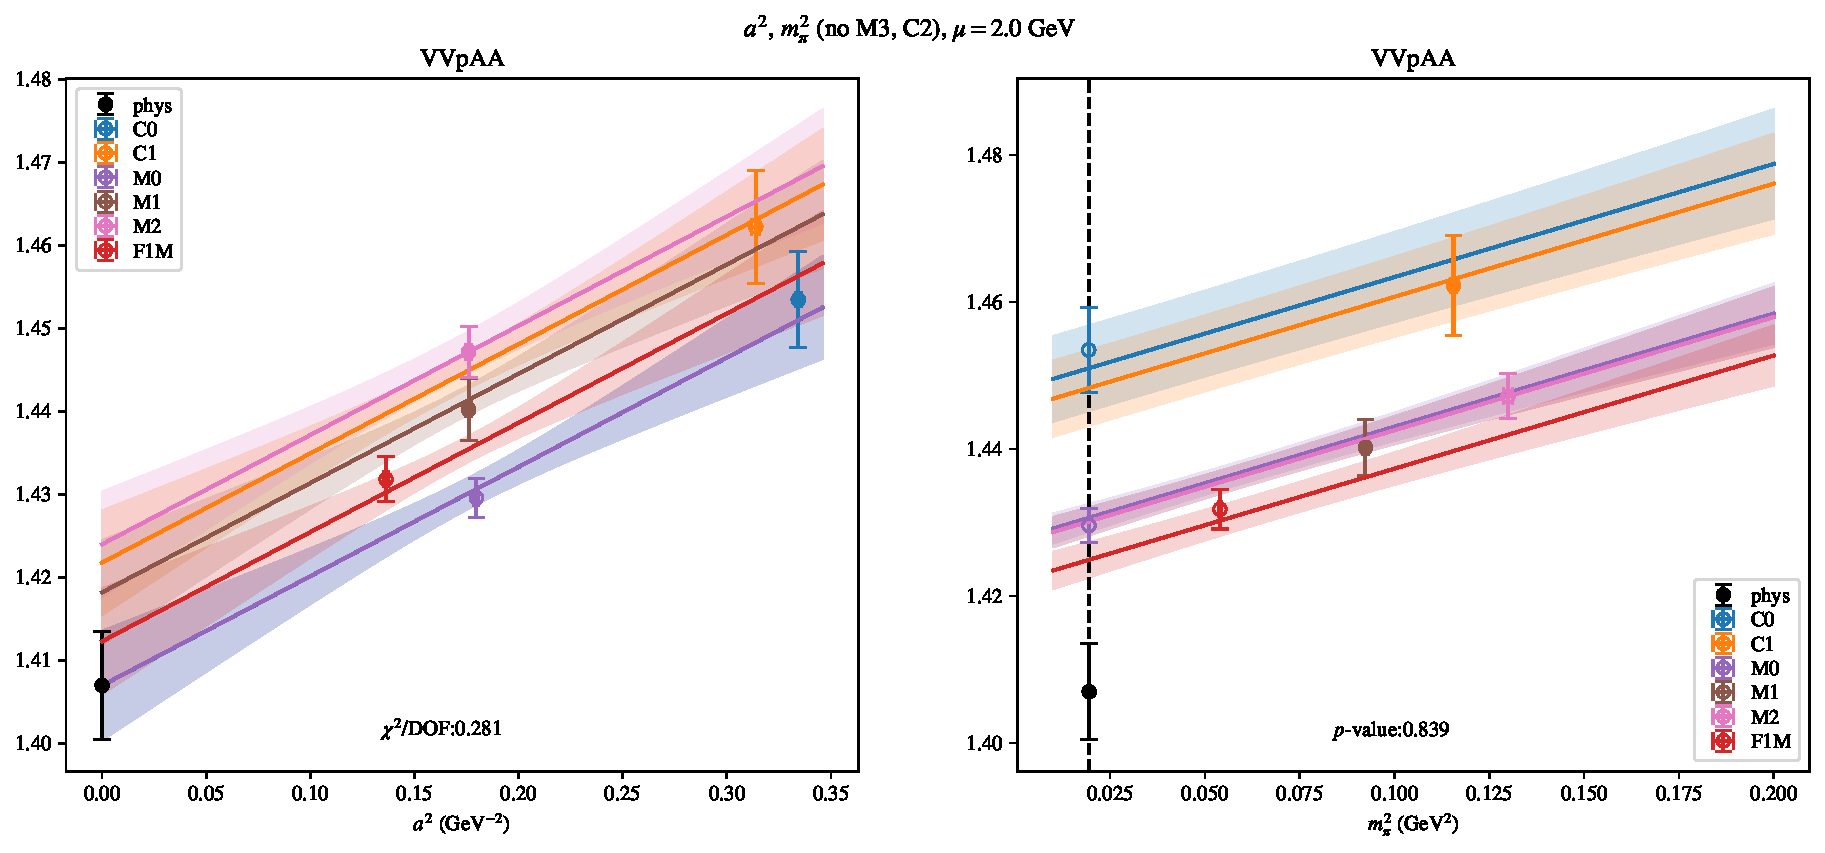
\includepdf[link, pages=-]{VVpAA/NPR/a2m2mcut_20.pdf}
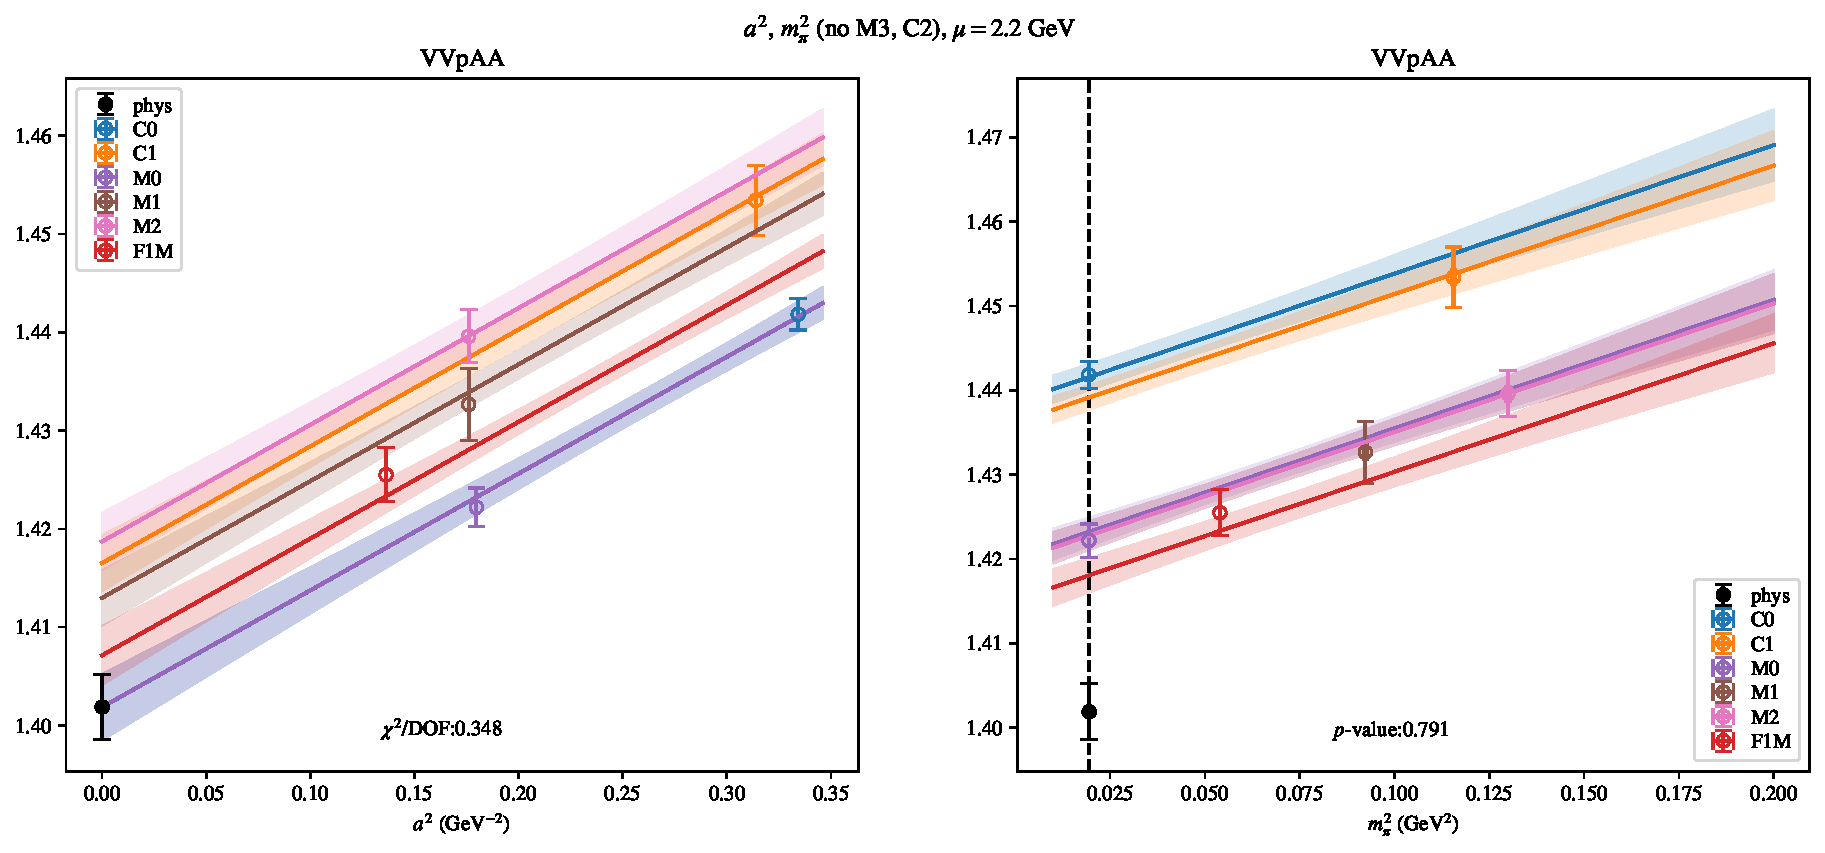
\includepdf[link, pages=-]{VVpAA/NPR/a2m2mcut_22.pdf}
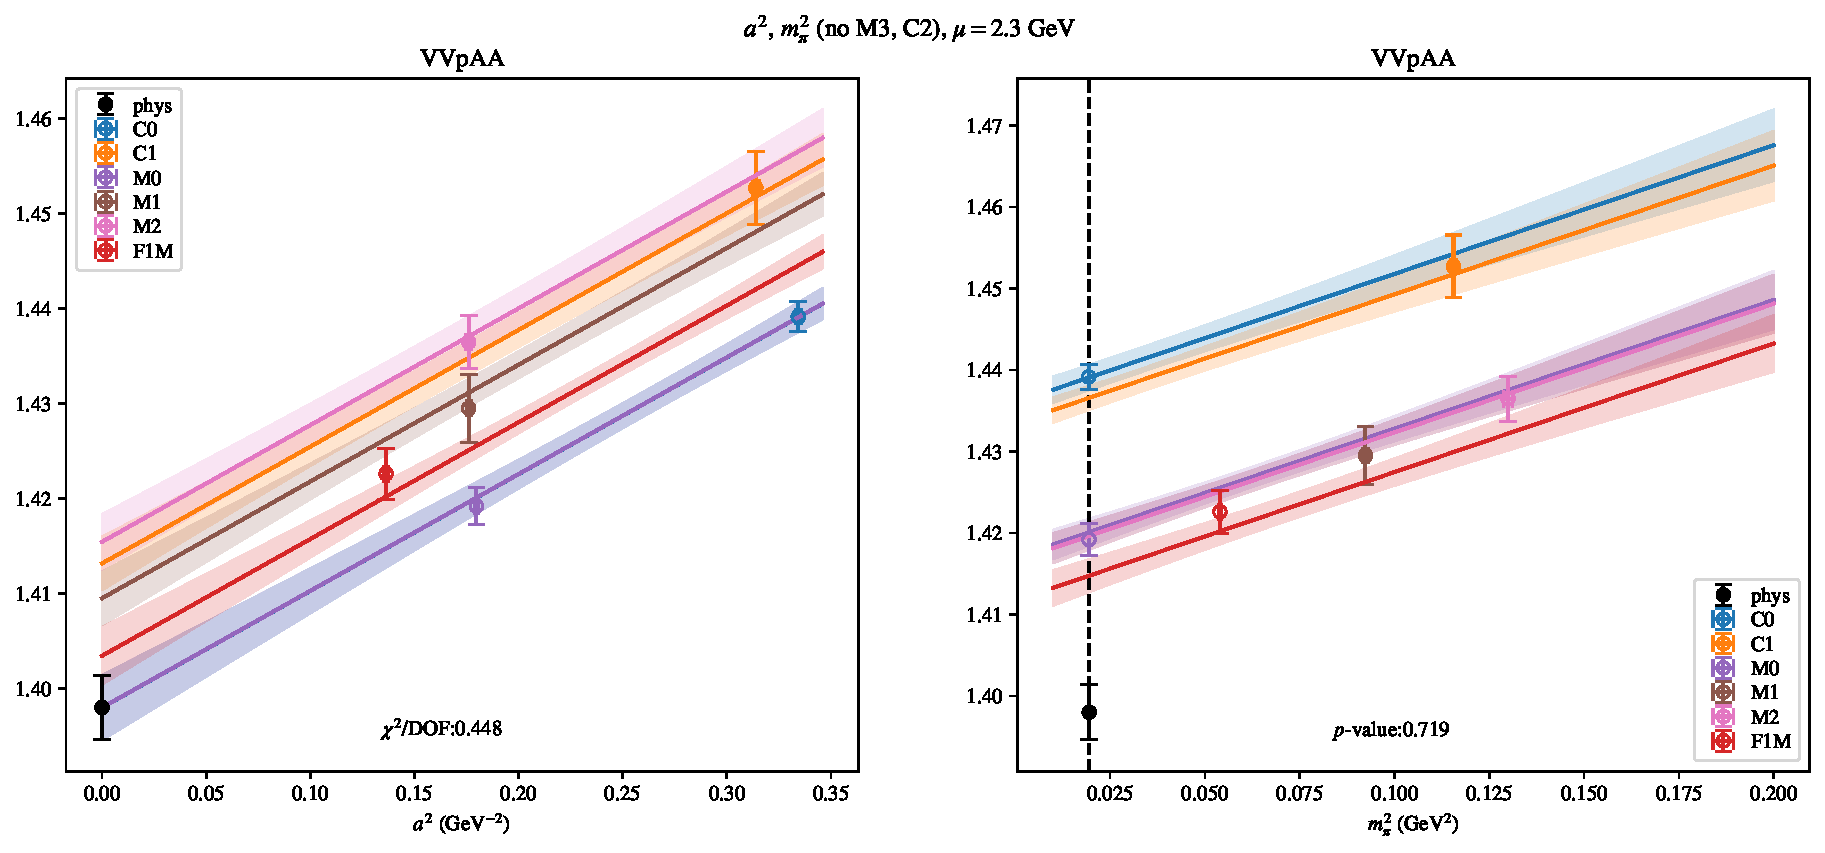
\includepdf[link, pages=-]{VVpAA/NPR/a2m2mcut_23.pdf}
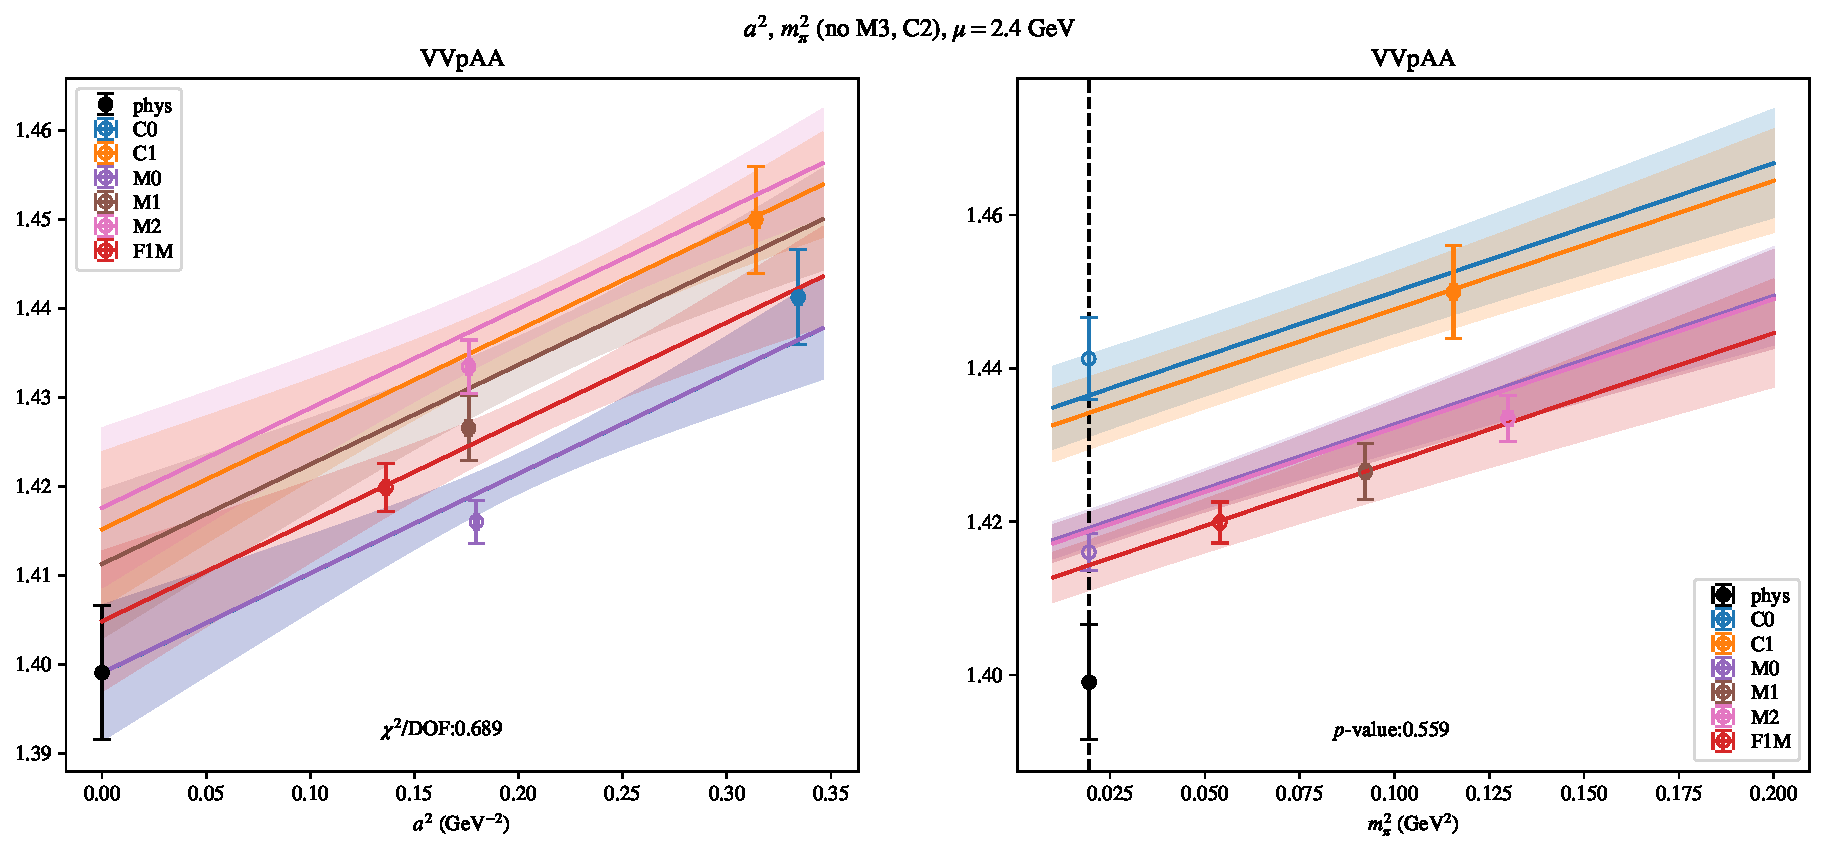
\includepdf[link, pages=-]{VVpAA/NPR/a2m2mcut_24.pdf}
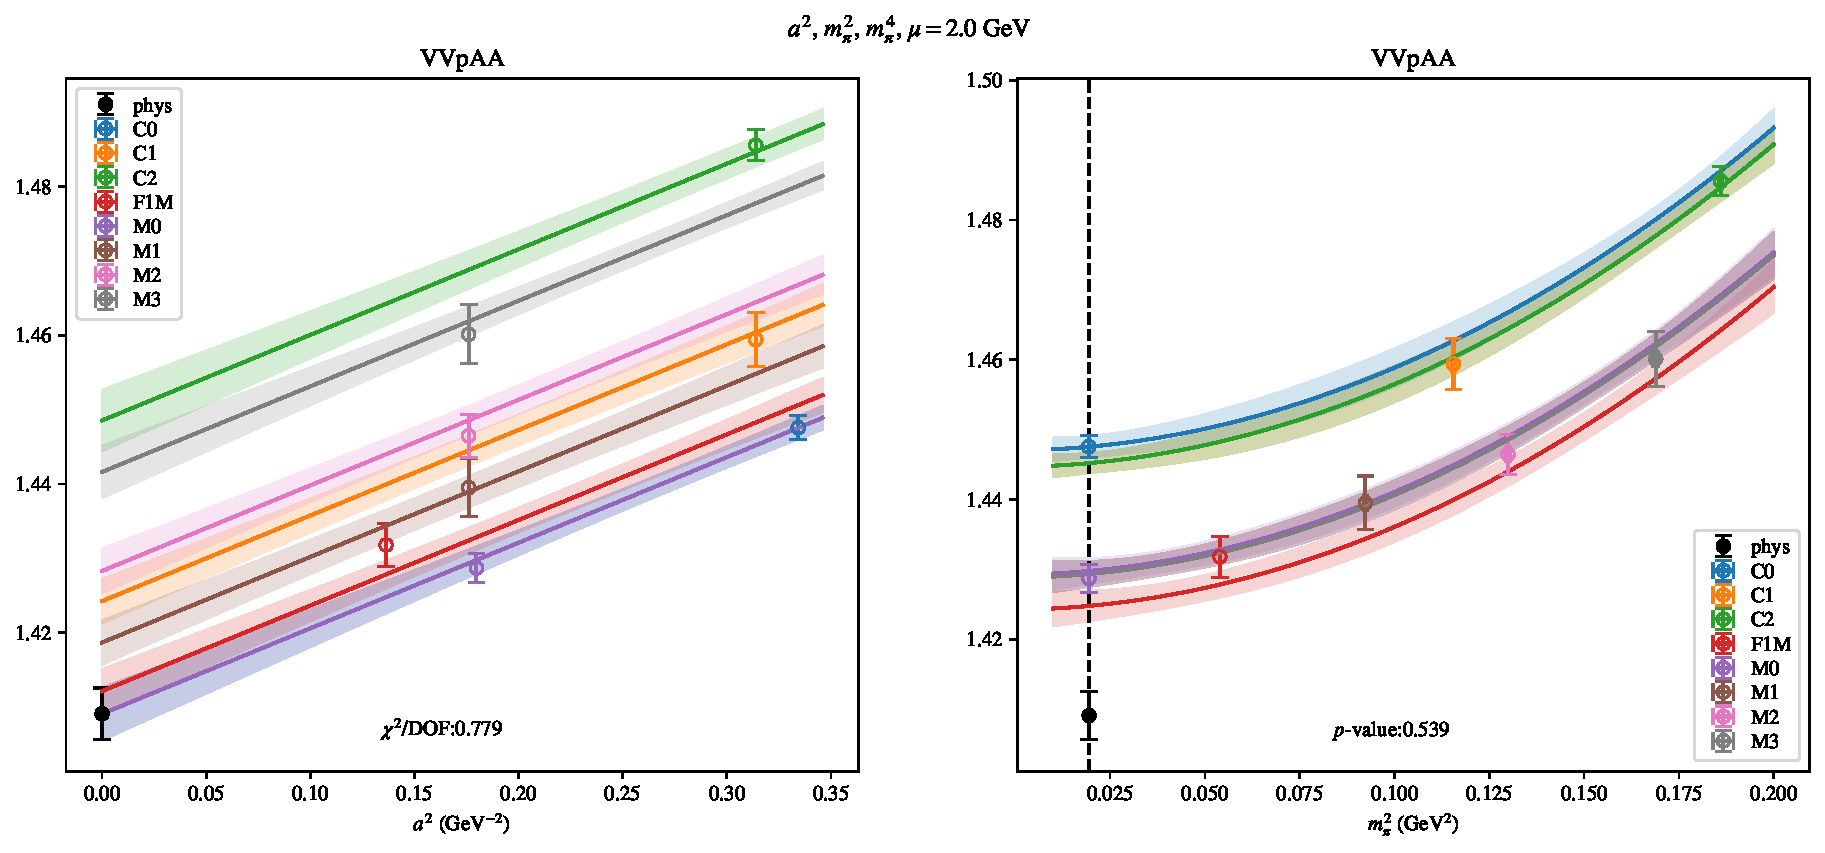
\includepdf[link, pages=-]{VVpAA/NPR/a2m2m4_20.pdf}
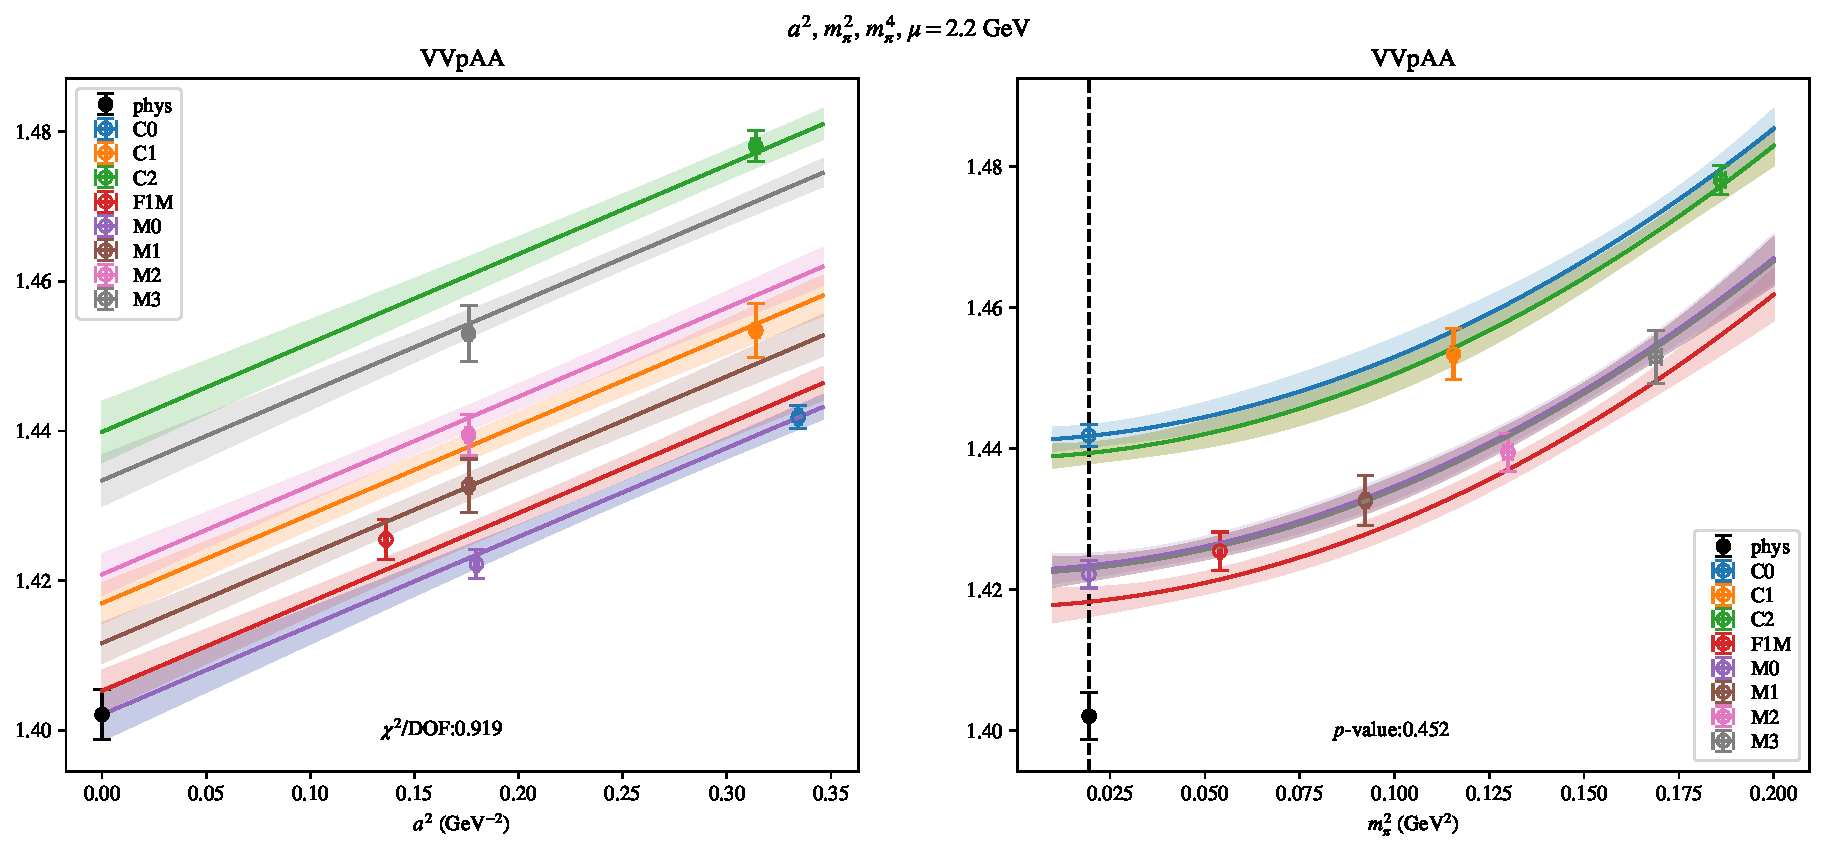
\includepdf[link, pages=-]{VVpAA/NPR/a2m2m4_22.pdf}
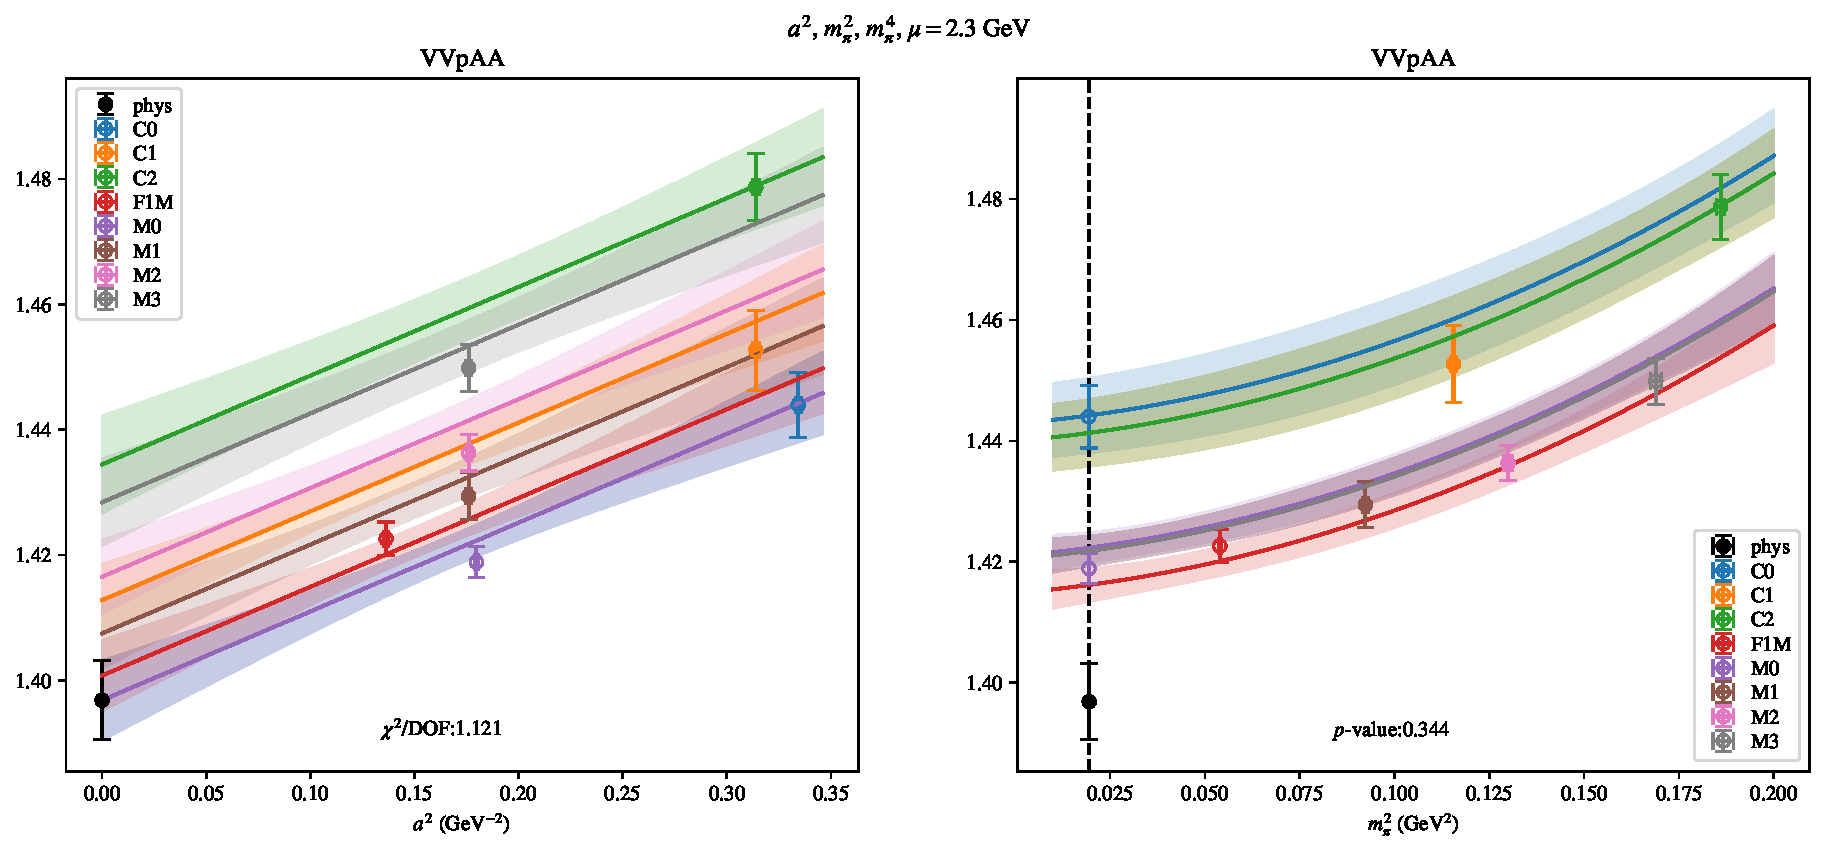
\includepdf[link, pages=-]{VVpAA/NPR/a2m2m4_23.pdf}
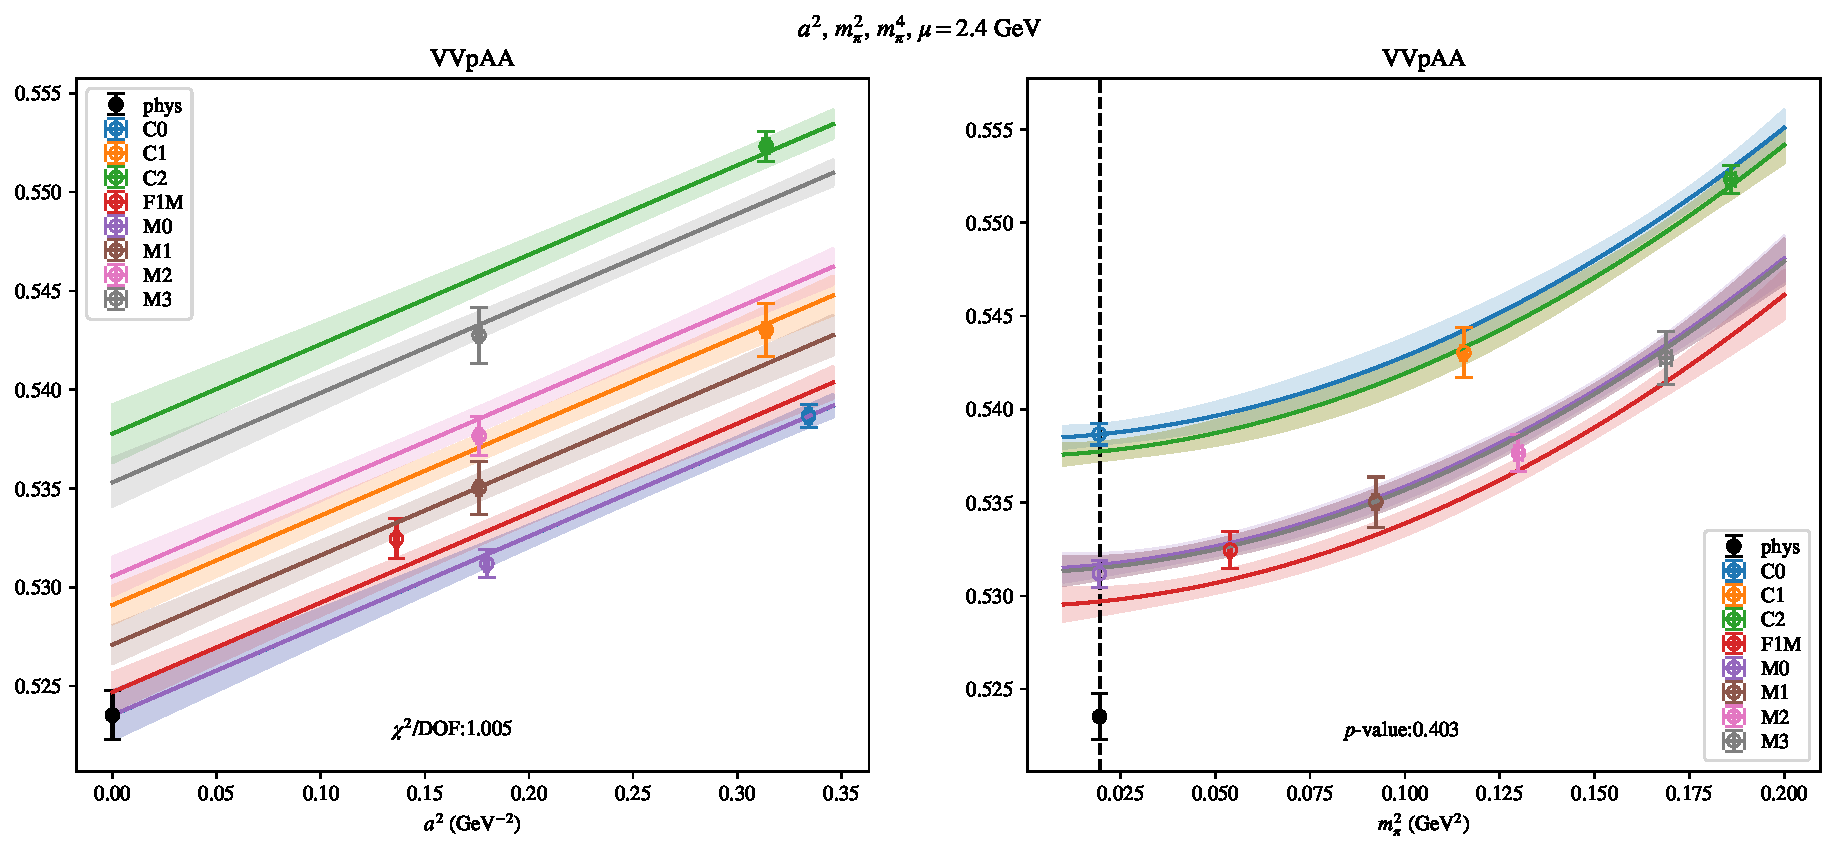
\includepdf[link, pages=-]{VVpAA/NPR/a2m2m4_24.pdf}
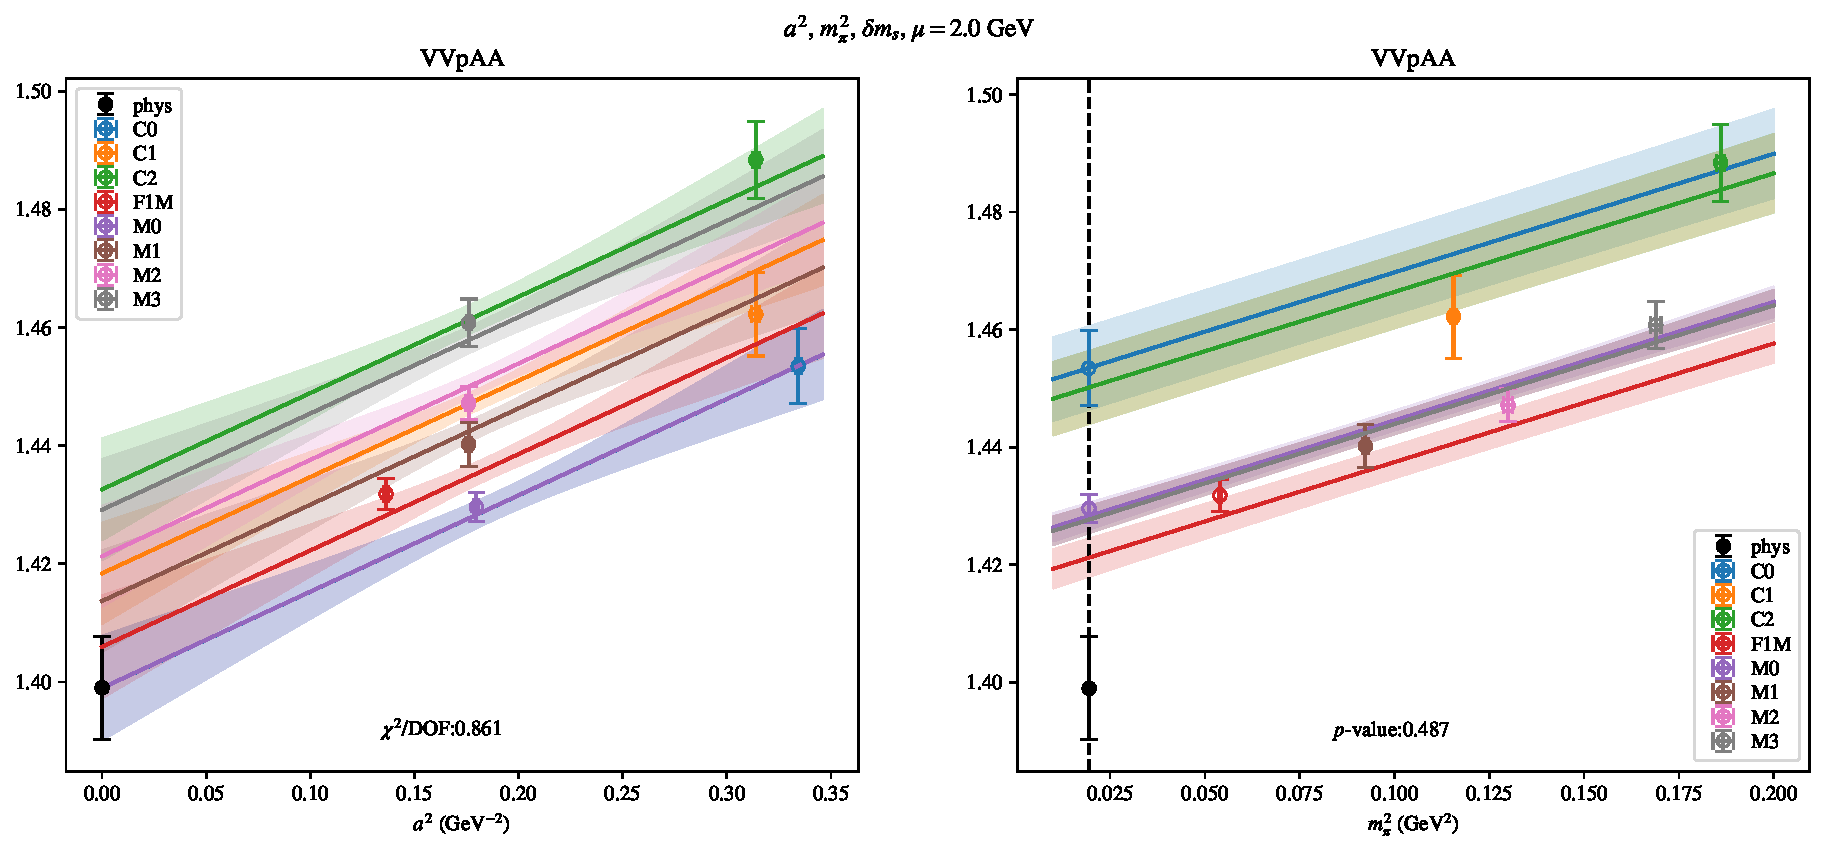
\includepdf[link, pages=-]{VVpAA/NPR/a2m2delm_20.pdf}
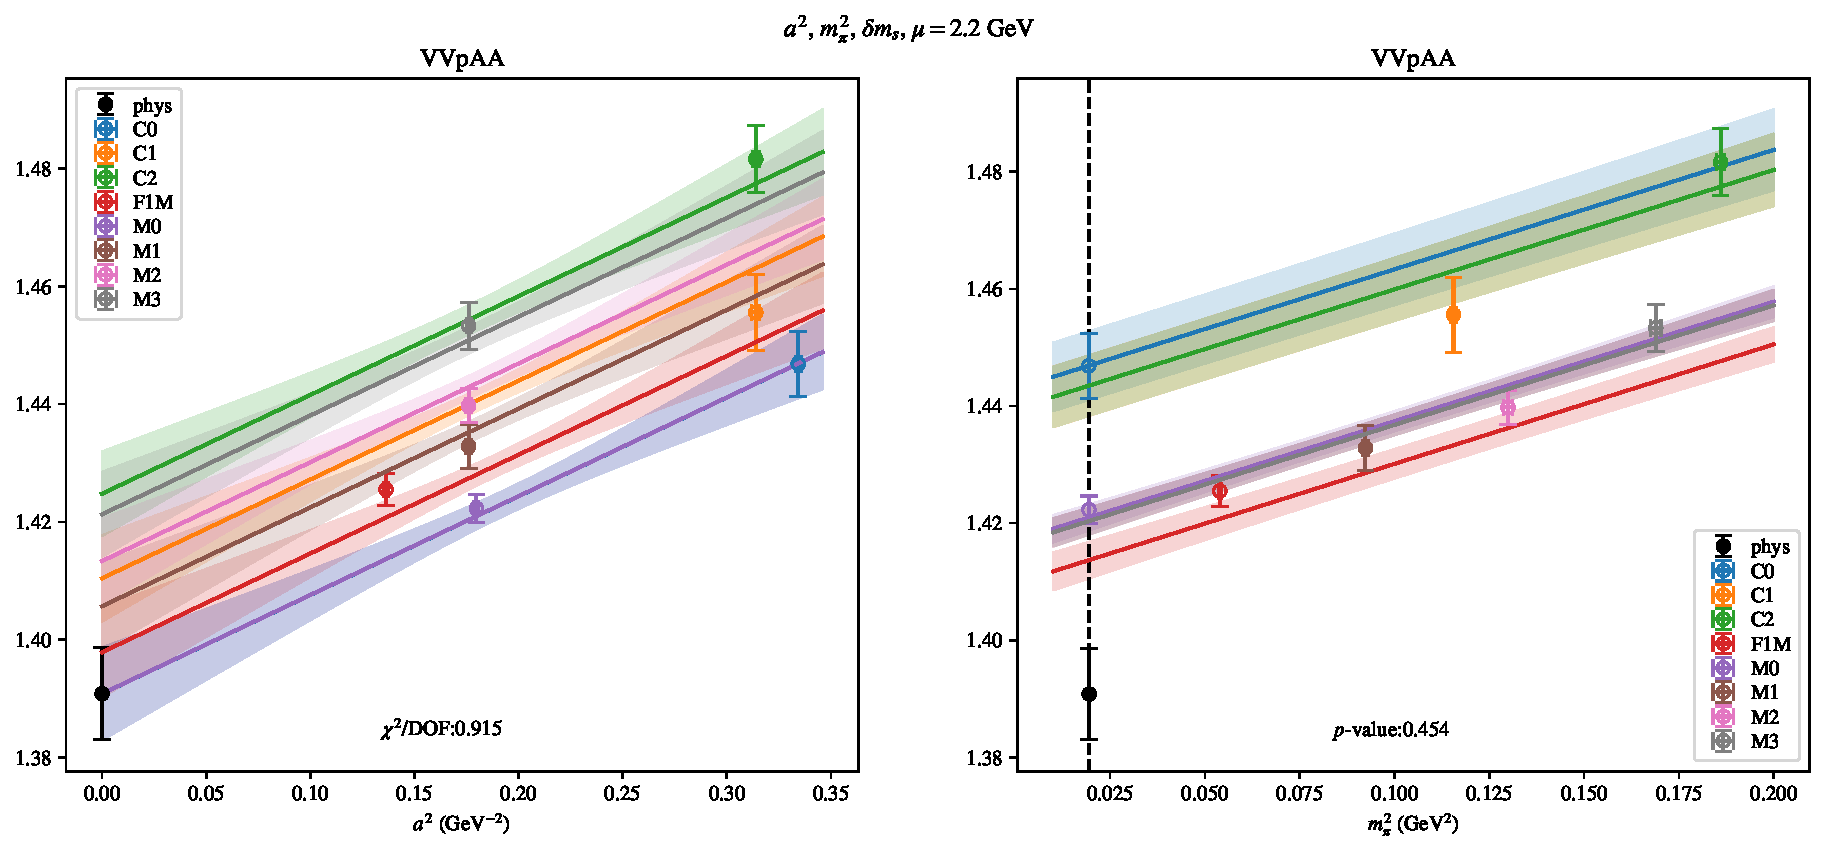
\includepdf[link, pages=-]{VVpAA/NPR/a2m2delm_22.pdf}
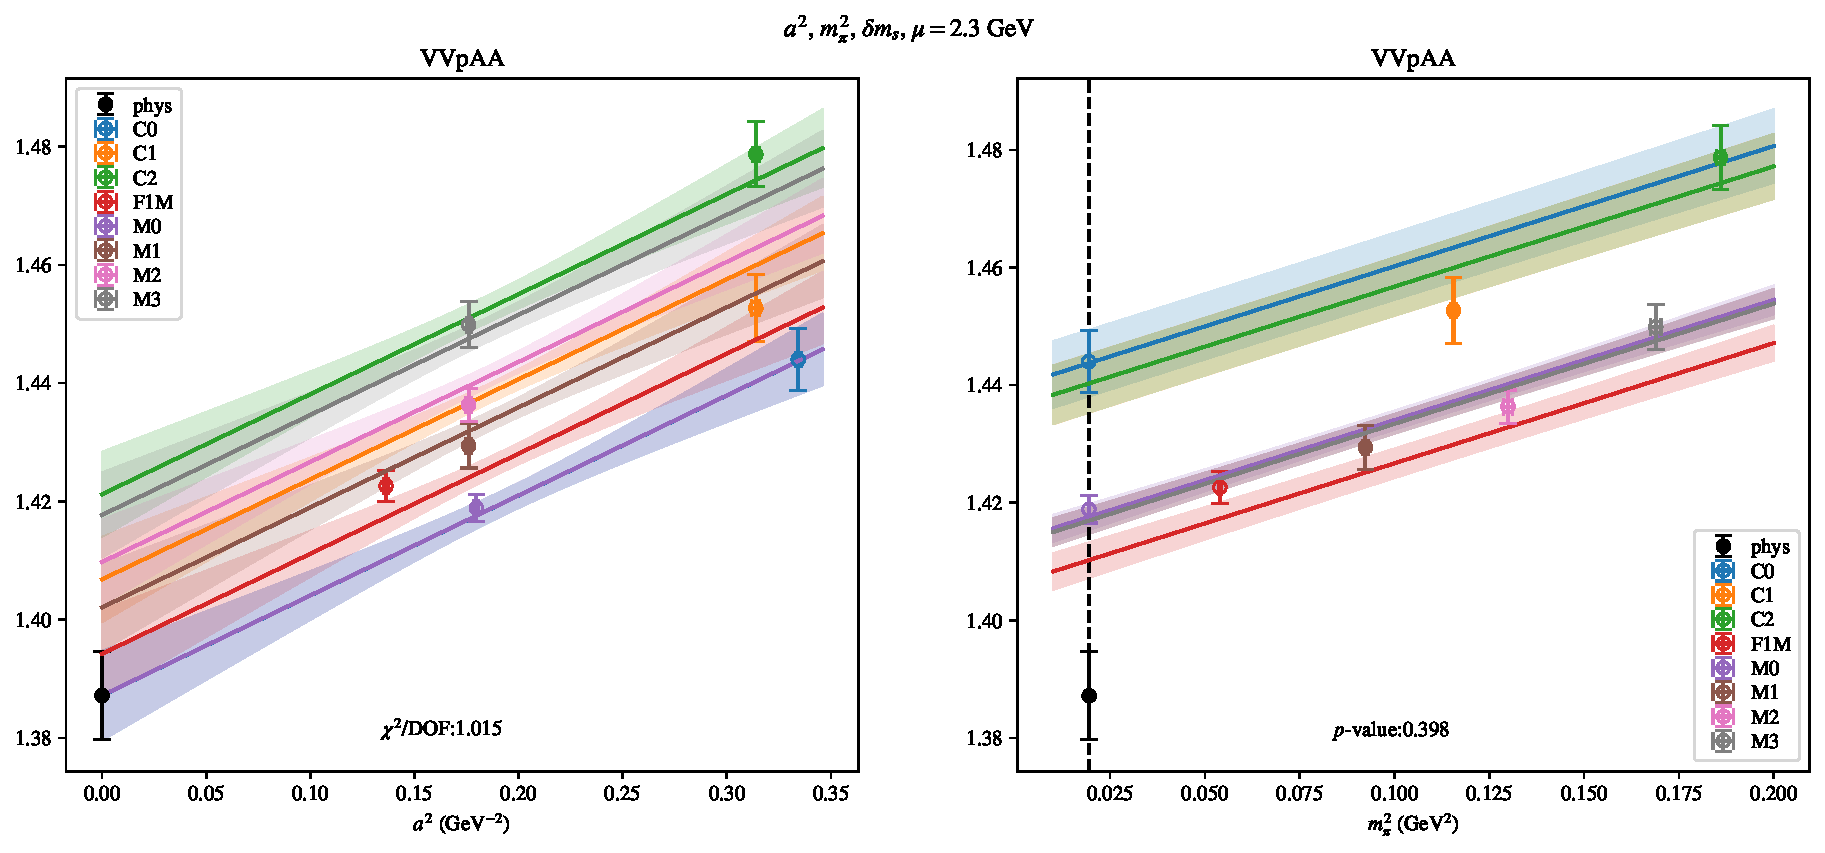
\includepdf[link, pages=-]{VVpAA/NPR/a2m2delm_23.pdf}
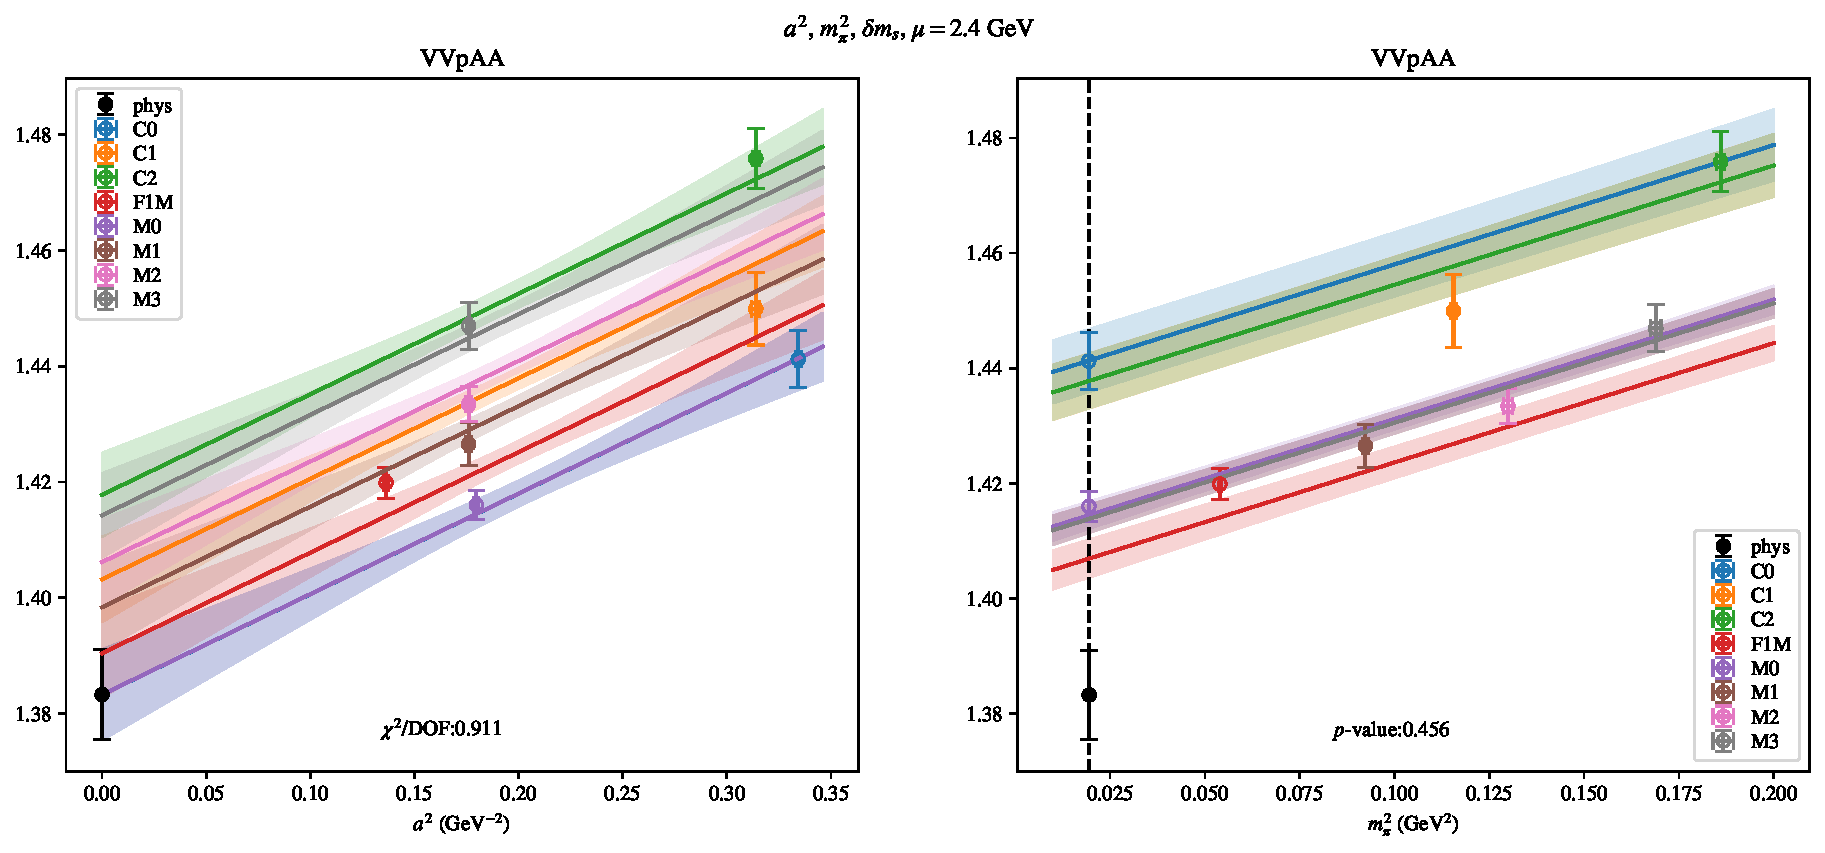
\includepdf[link, pages=-]{VVpAA/NPR/a2m2delm_24.pdf}
\clearpage
\section{$\mathcal{B}_2$}
\begin{table}[h!]
\begin{center}
\begin{tabular}{|c|c|c|c|c|c|c|}
\hline
$\mu$ (GeV) & $a^2$, $m_\pi^2$& $a^2$, $m_\pi^2$ (no C)& $a^2$, $a^4$, $m_\pi^2$& $a^2$, $m_\pi^2$ (no M3, C2)& $a^2$, $m_\pi^2$, $m_\pi^4$& $a^2$, $m_\pi^2$, $\delta m_s$\\
\hline
2.0& \hyperlink{VVmAA/NPR/a2m2_20.pdf.1}{\textbf{-0.991(15)}: 10.845 (0.0)} & \hyperlink{VVmAA/NPR/a2m2noC_20.pdf.1}{\textbf{-0.931(87)}: 1.836 (0.159)} & \hyperlink{VVmAA/NPR/a2a4m2_20.pdf.1}{\textbf{-0.89(12)}: 1.829 (0.12)} & \hyperlink{VVmAA/NPR/a2m2mcut_20.pdf.1}{\textbf{-0.992(16)}: 16.944 (0.0)} & \hyperlink{VVmAA/NPR/a2m2m4_20.pdf.1}{\textbf{-0.993(16)}: 10.337 (0.0)} & \hyperlink{VVmAA/NPR/a2m2delm_20.pdf.1}{\textbf{-0.995(17)}: 2.1 (0.078)}\\
2.2& \hyperlink{VVmAA/NPR/a2m2_22.pdf.1}{\textbf{-1.005(15)}: 10.324 (0.0)} & \hyperlink{VVmAA/NPR/a2m2noC_22.pdf.1}{\textbf{-0.950(86)}: 2.883 (0.056)} & \hyperlink{VVmAA/NPR/a2a4m2_22.pdf.1}{\textbf{-0.92(13)}: 2.555 (0.037)} & \hyperlink{VVmAA/NPR/a2m2mcut_22.pdf.1}{\textbf{-1.006(16)}: 14.623 (0.0)} & \hyperlink{VVmAA/NPR/a2m2m4_22.pdf.1}{\textbf{-1.007(16)}: 8.756 (0.0)} & \hyperlink{VVmAA/NPR/a2m2delm_22.pdf.1}{\textbf{-1.008(16)}: 3.189 (0.013)}\\
2.3& \hyperlink{VVmAA/NPR/a2m2_23.pdf.1}{\textbf{-1.012(15)}: 10.333 (0.0)} & \hyperlink{VVmAA/NPR/a2m2noC_23.pdf.1}{\textbf{-0.956(85)}: 3.098 (0.045)} & \hyperlink{VVmAA/NPR/a2a4m2_23.pdf.1}{\textbf{-0.92(13)}: 2.44 (0.045)} & \hyperlink{VVmAA/NPR/a2m2mcut_23.pdf.1}{\textbf{-1.012(16)}: 14.827 (0.0)} & \hyperlink{VVmAA/NPR/a2m2m4_23.pdf.1}{\textbf{-1.014(16)}: 9.091 (0.0)} & \hyperlink{VVmAA/NPR/a2m2delm_23.pdf.1}{\textbf{-1.015(16)}: 3.286 (0.011)}\\
2.4& \hyperlink{VVmAA/NPR/a2m2_24.pdf.1}{\textbf{-1.016(15)}: 9.457 (0.0)} & \hyperlink{VVmAA/NPR/a2m2noC_24.pdf.1}{\textbf{-0.964(84)}: 3.107 (0.045)} & \hyperlink{VVmAA/NPR/a2a4m2_24.pdf.1}{\textbf{-0.93(12)}: 2.631 (0.032)} & \hyperlink{VVmAA/NPR/a2m2mcut_24.pdf.1}{\textbf{-1.017(16)}: 13.426 (0.0)} & \hyperlink{VVmAA/NPR/a2m2m4_24.pdf.1}{\textbf{-1.018(16)}: 8.409 (0.0)} & \hyperlink{VVmAA/NPR/a2m2delm_24.pdf.1}{\textbf{-1.019(16)}: 3.033 (0.016)}\\
\hline
\end{tabular}
\caption{Physical point value from chiral and continuum extrapolation at renormalisation scale $\mu$. Entries are \textbf{value(error)}: $\chi^2/\text{DOF}$ ($p$-value).}
\end{center}
\end{table}
\begin{table}[h!]
\begin{center}
\begin{tabular}{|c c|c|c|c|c|c|c|}
\hline
$\mu$ (GeV) &  & $a^2$, $m_\pi^2$& $a^2$, $m_\pi^2$ (no C)& $a^2$, $a^4$, $m_\pi^2$& $a^2$, $m_\pi^2$ (no M3, C2)& $a^2$, $m_\pi^2$, $m_\pi^4$& $a^2$, $m_\pi^2$, $\delta m_s$\\
\hline
\multirow{2}{0.5in}{2.0} & $\alpha$ & -0.184(56)& 0.176(54)& 0.72(13)& -0.185(57)& -0.189(57)& -0.195(59)\\
 & $\beta$ & 0.00105(14)& 0.00114(25)& 0.00085(17)& 0.00068(25)& -0.0015(75)& 0.00081(14)\\
\hline
\multirow{2}{0.5in}{2.2} & $\alpha$ & -0.224(54)& 0.099(52)& 0.58(13)& -0.225(56)& -0.229(56)& -0.233(58)\\
 & $\beta$ & 0.00116(13)& 0.00119(23)& 0.00097(16)& 0.00066(23)& -0.0014(70)& 0.00094(14)\\
\hline
\multirow{2}{0.5in}{2.3} & $\alpha$ & -0.246(54)& 0.070(51)& 0.54(13)& -0.247(56)& -0.251(56)& -0.255(58)\\
 & $\beta$ & 0.00116(13)& 0.00119(22)& 0.00098(15)& 0.00070(23)& -0.0012(68)& 0.00094(13)\\
\hline
\multirow{2}{0.5in}{2.4} & $\alpha$ & -0.265(54)& 0.031(50)& 0.46(13)& -0.266(56)& -0.271(57)& -0.273(58)\\
 & $\beta$ & 0.00111(13)& 0.00120(21)& 0.00095(15)& 0.00069(22)& -0.0011(67)& 0.00091(13)\\
\hline
\end{tabular}
\caption{Fit values of coefficients in $Q = Q_{phys} + \mathbf{\alpha} a^2 + \mathbf{\beta}\left(\frac{m_\pi^2}{f_\pi^2}-\frac{m_{\pi,PDG}^2}{f_\pi^2}\right) + \ldots$.}
\end{center}
\end{table}
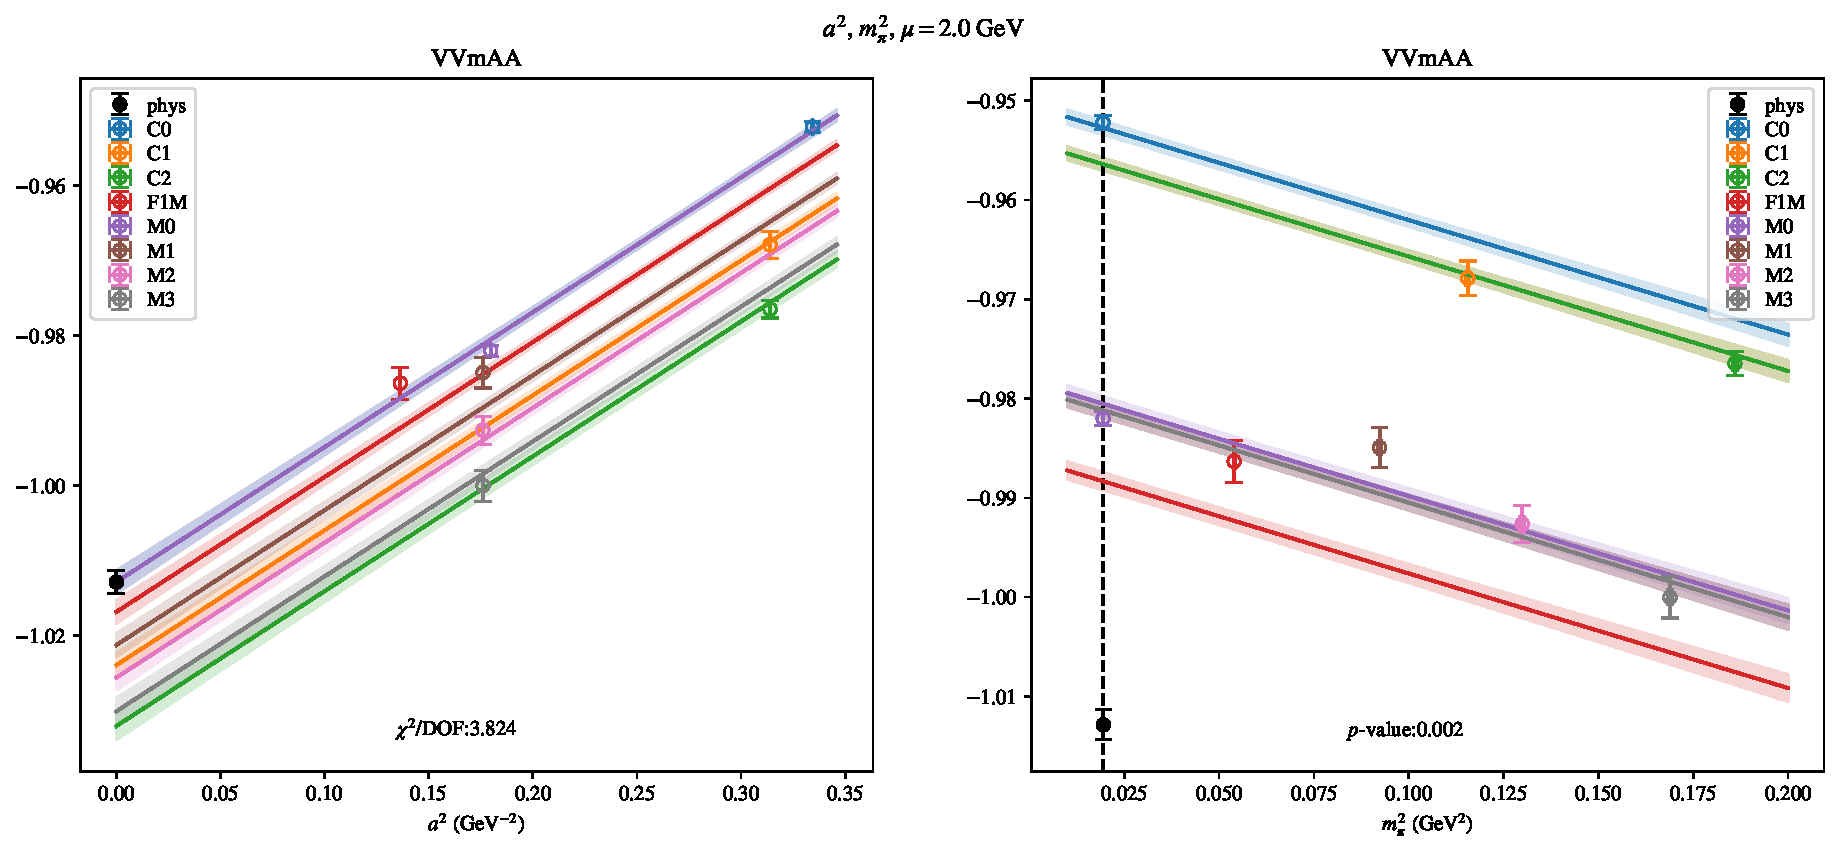
\includepdf[link, pages=-]{VVmAA/NPR/a2m2_20.pdf}
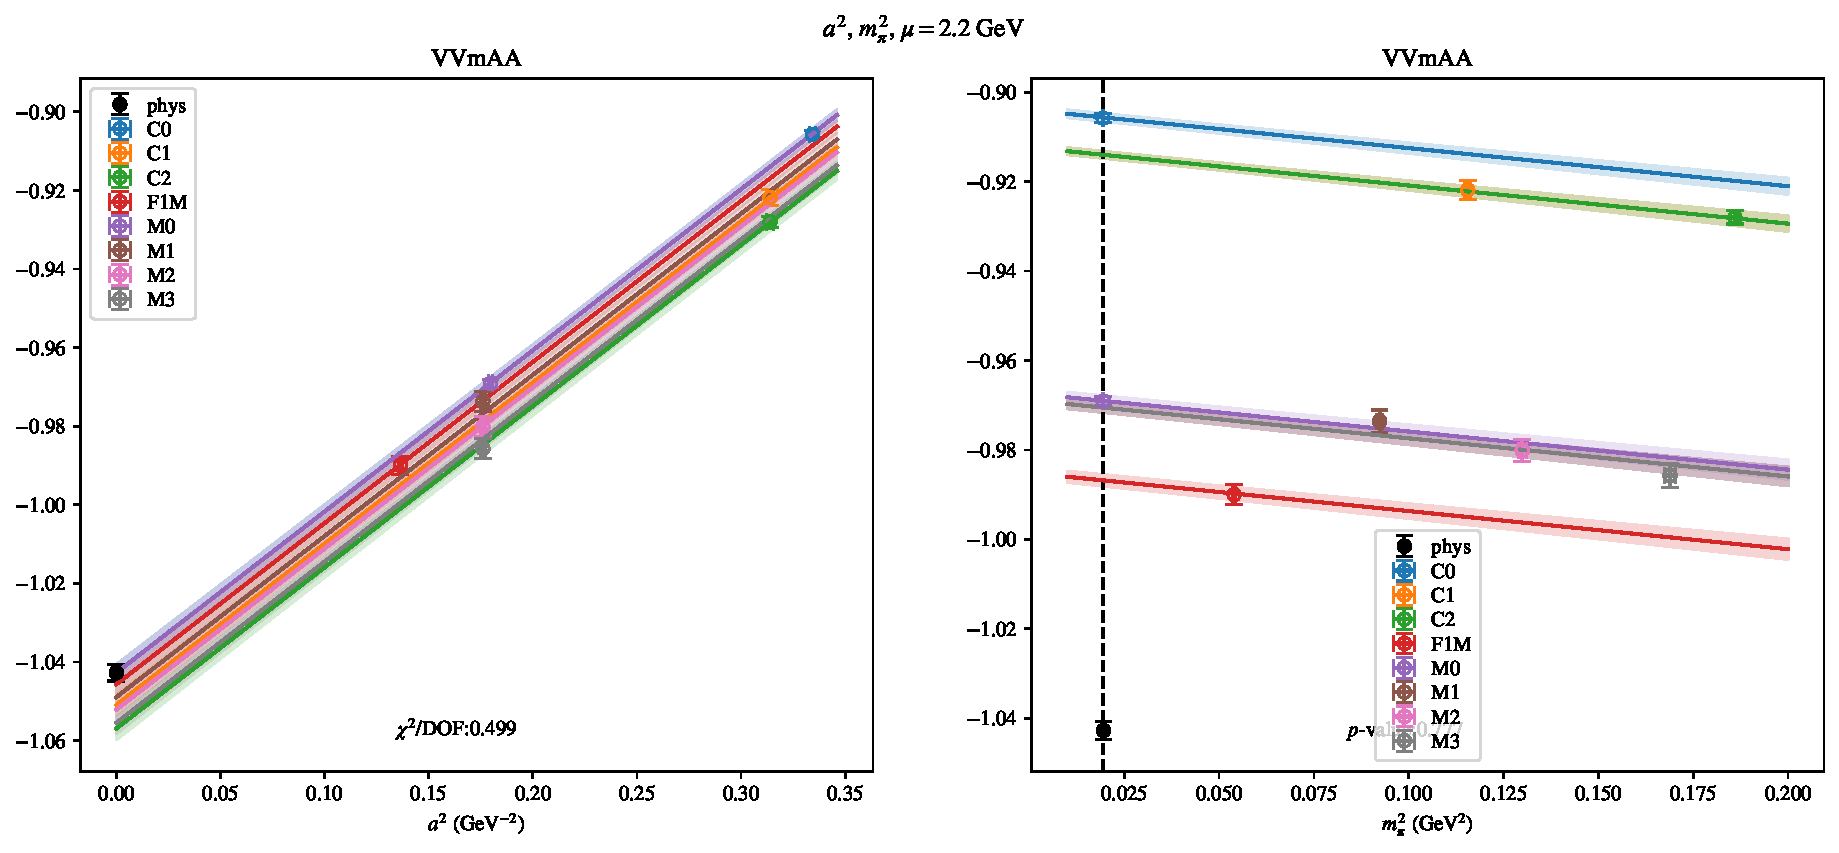
\includepdf[link, pages=-]{VVmAA/NPR/a2m2_22.pdf}
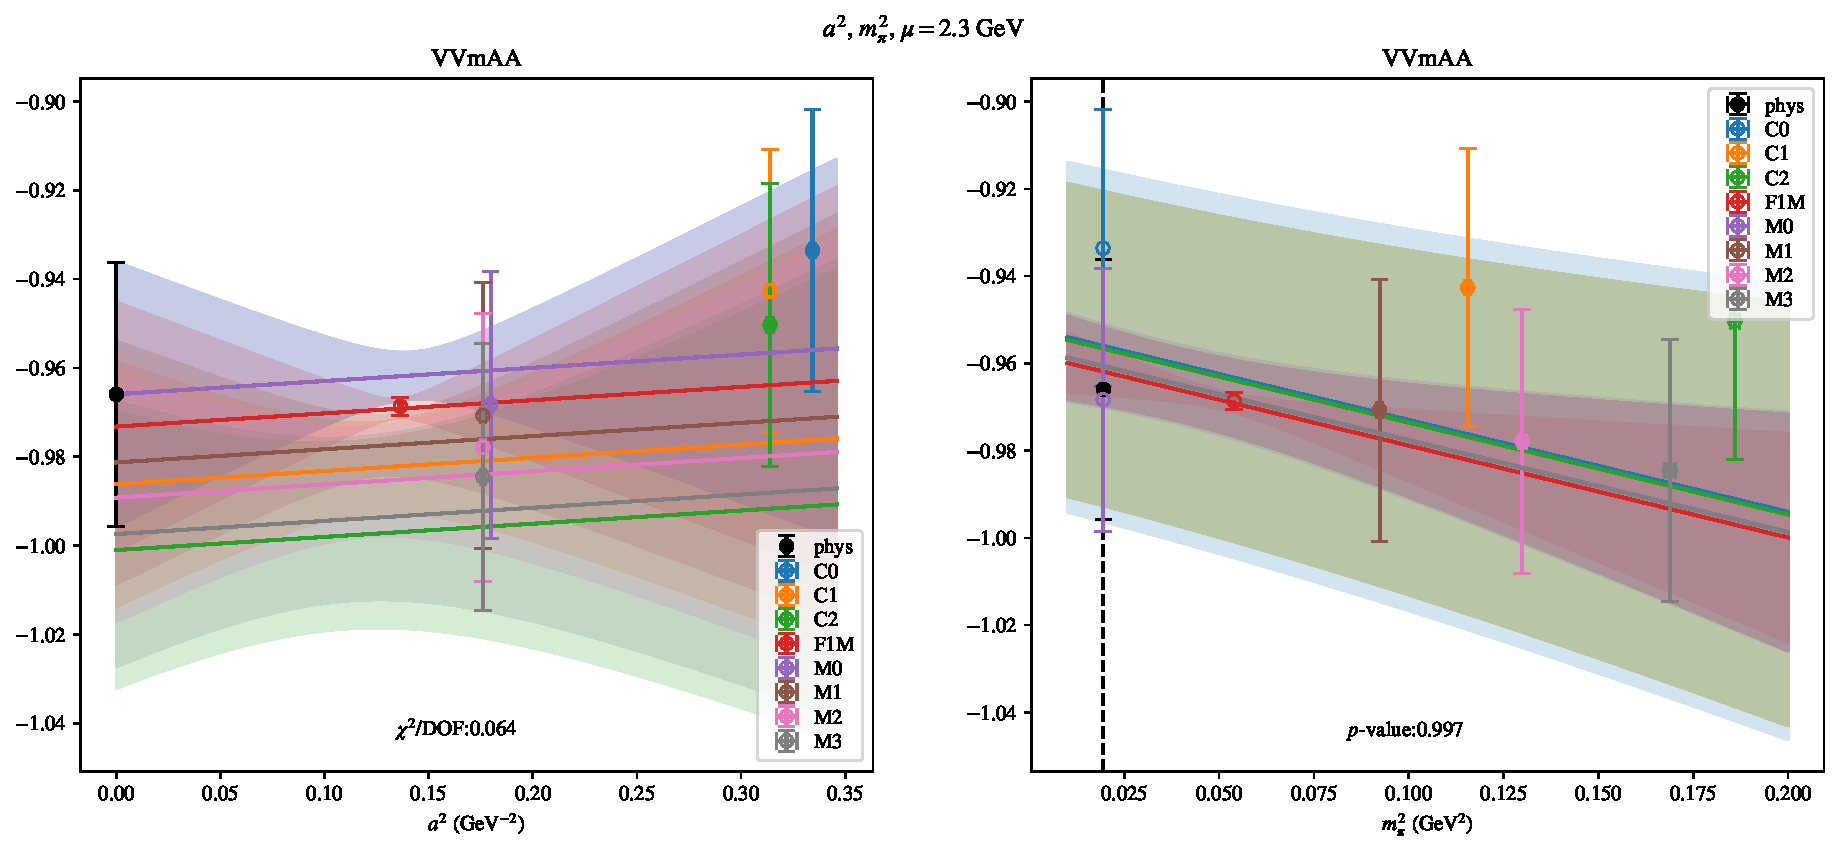
\includepdf[link, pages=-]{VVmAA/NPR/a2m2_23.pdf}
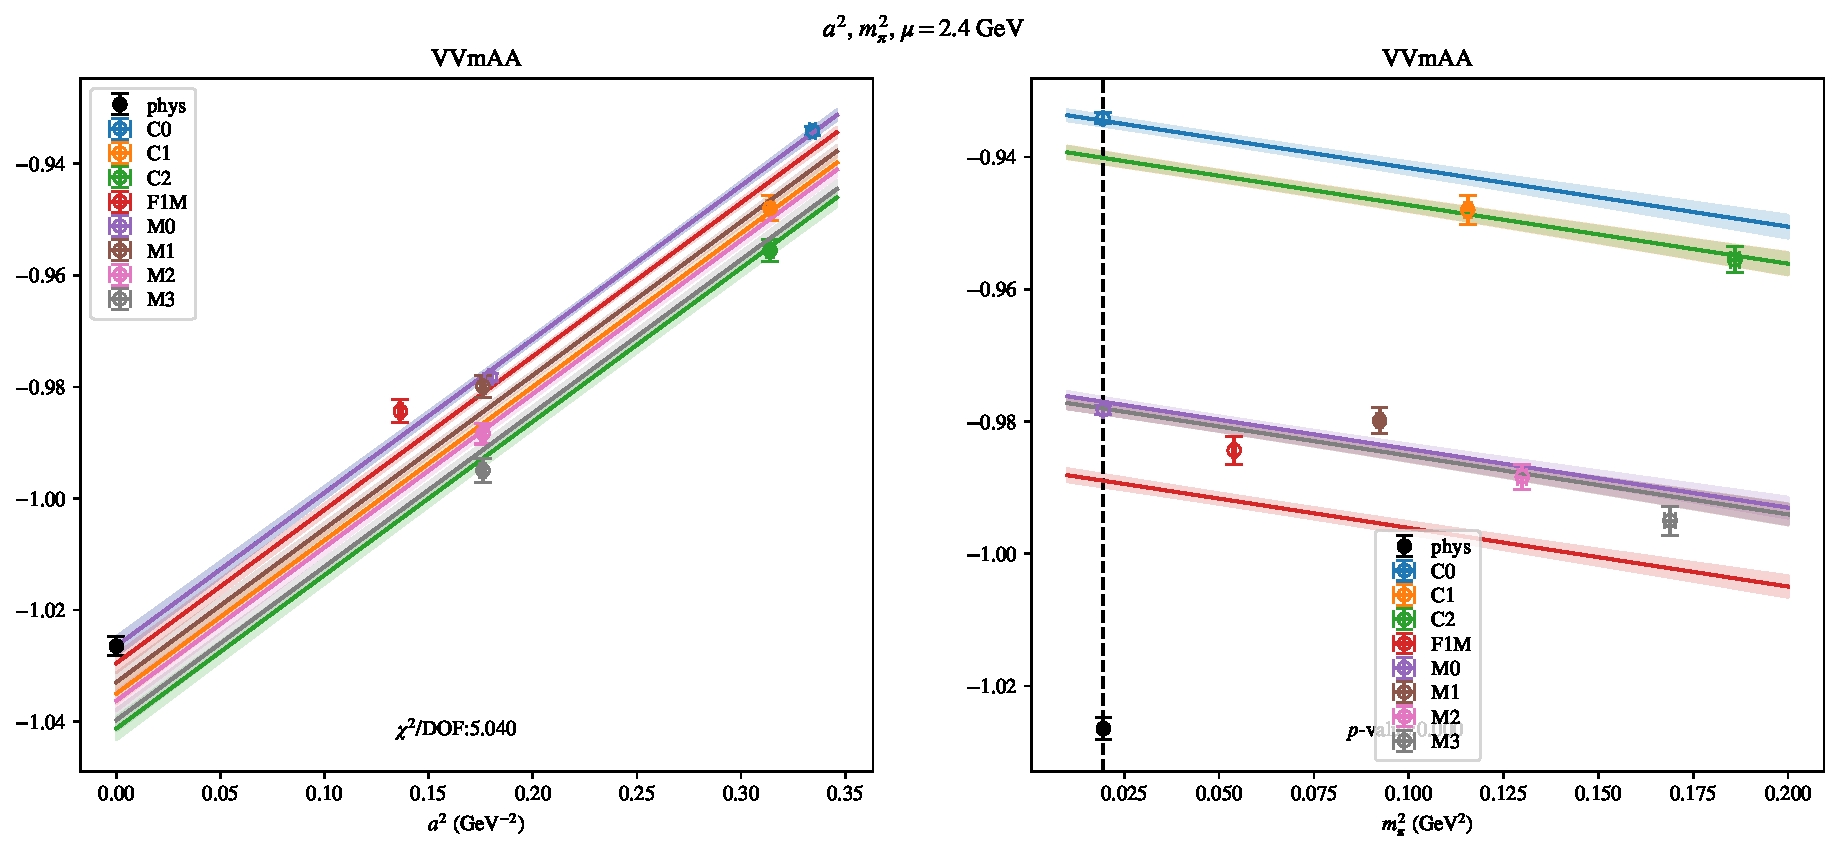
\includepdf[link, pages=-]{VVmAA/NPR/a2m2_24.pdf}
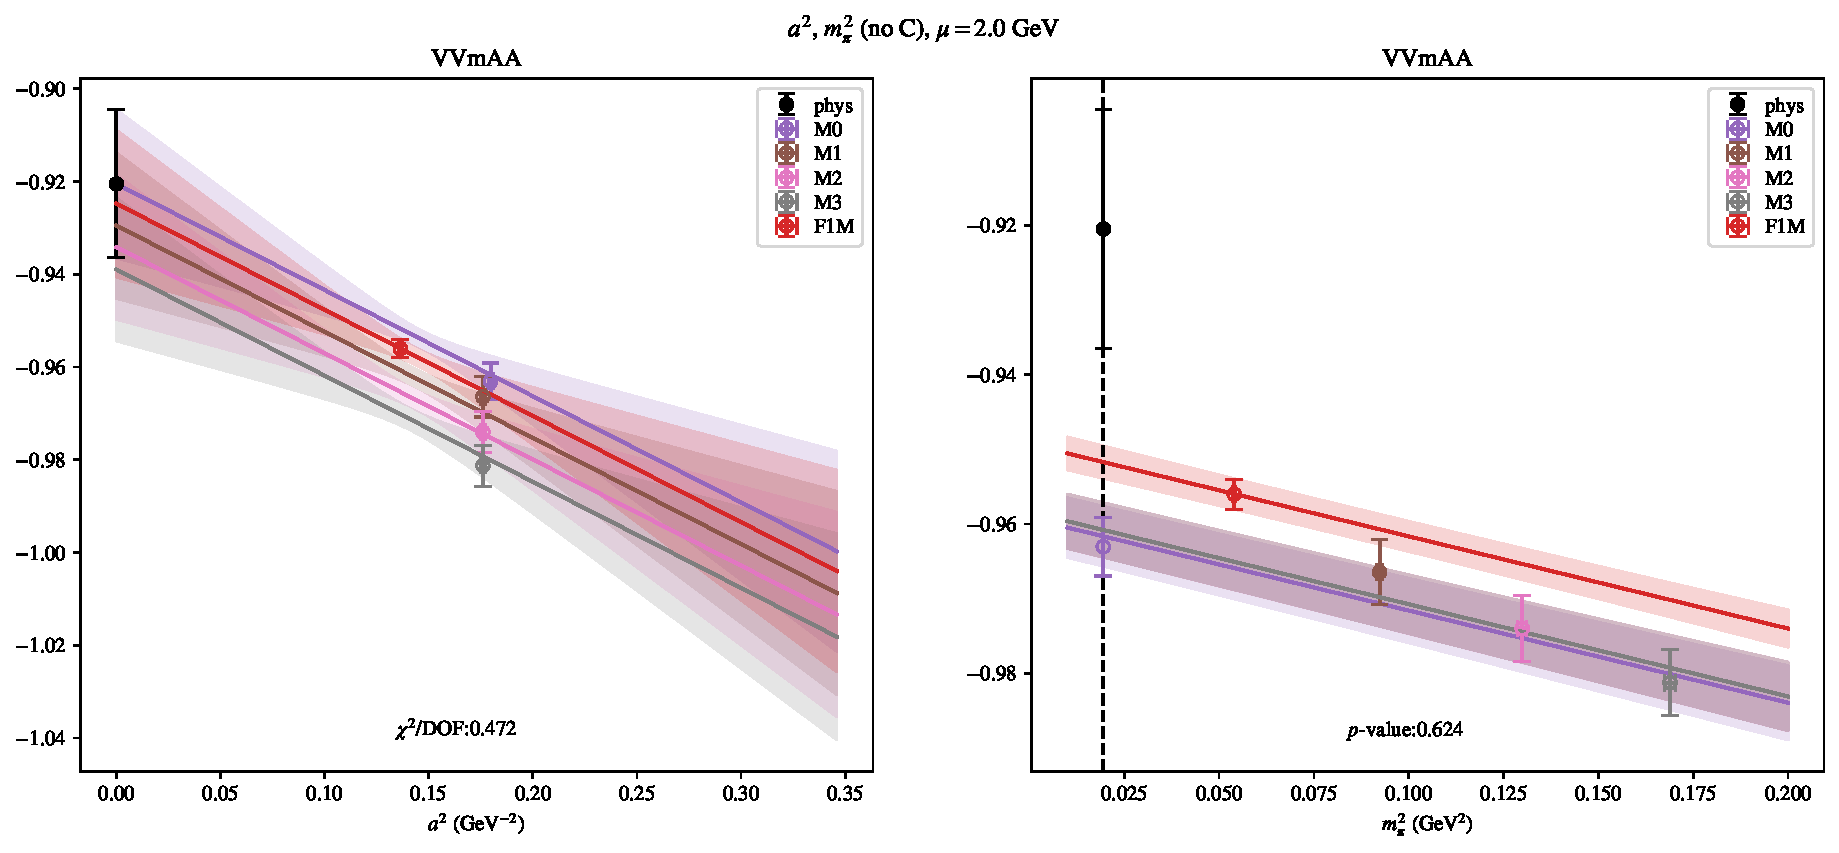
\includepdf[link, pages=-]{VVmAA/NPR/a2m2noC_20.pdf}
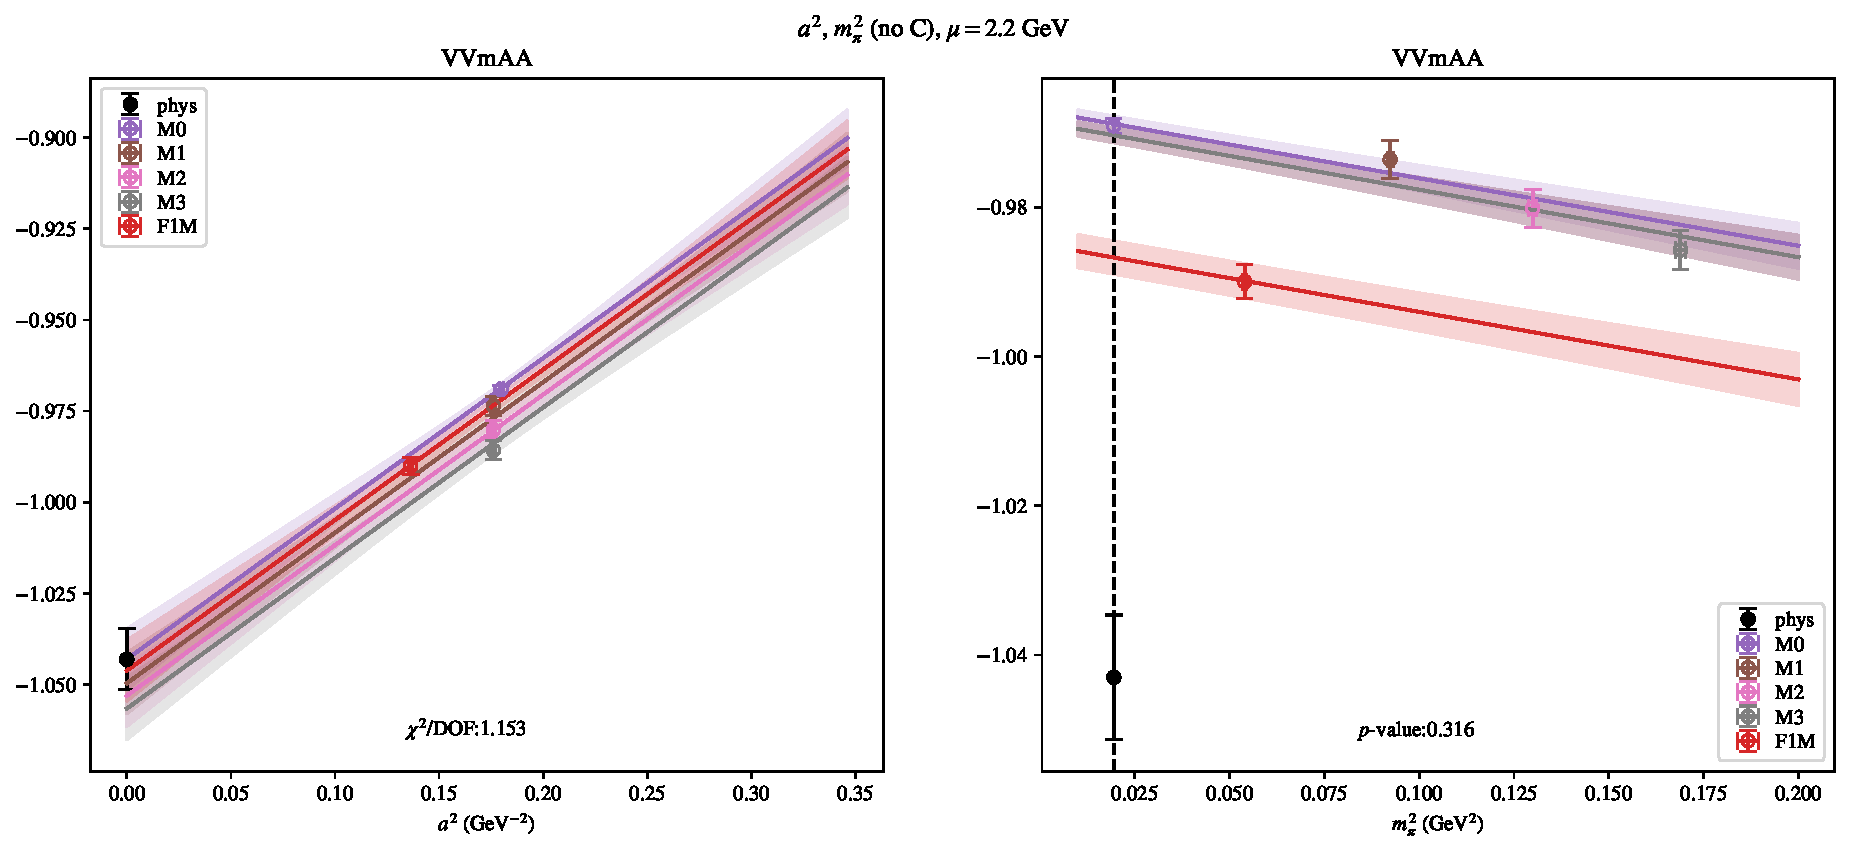
\includepdf[link, pages=-]{VVmAA/NPR/a2m2noC_22.pdf}
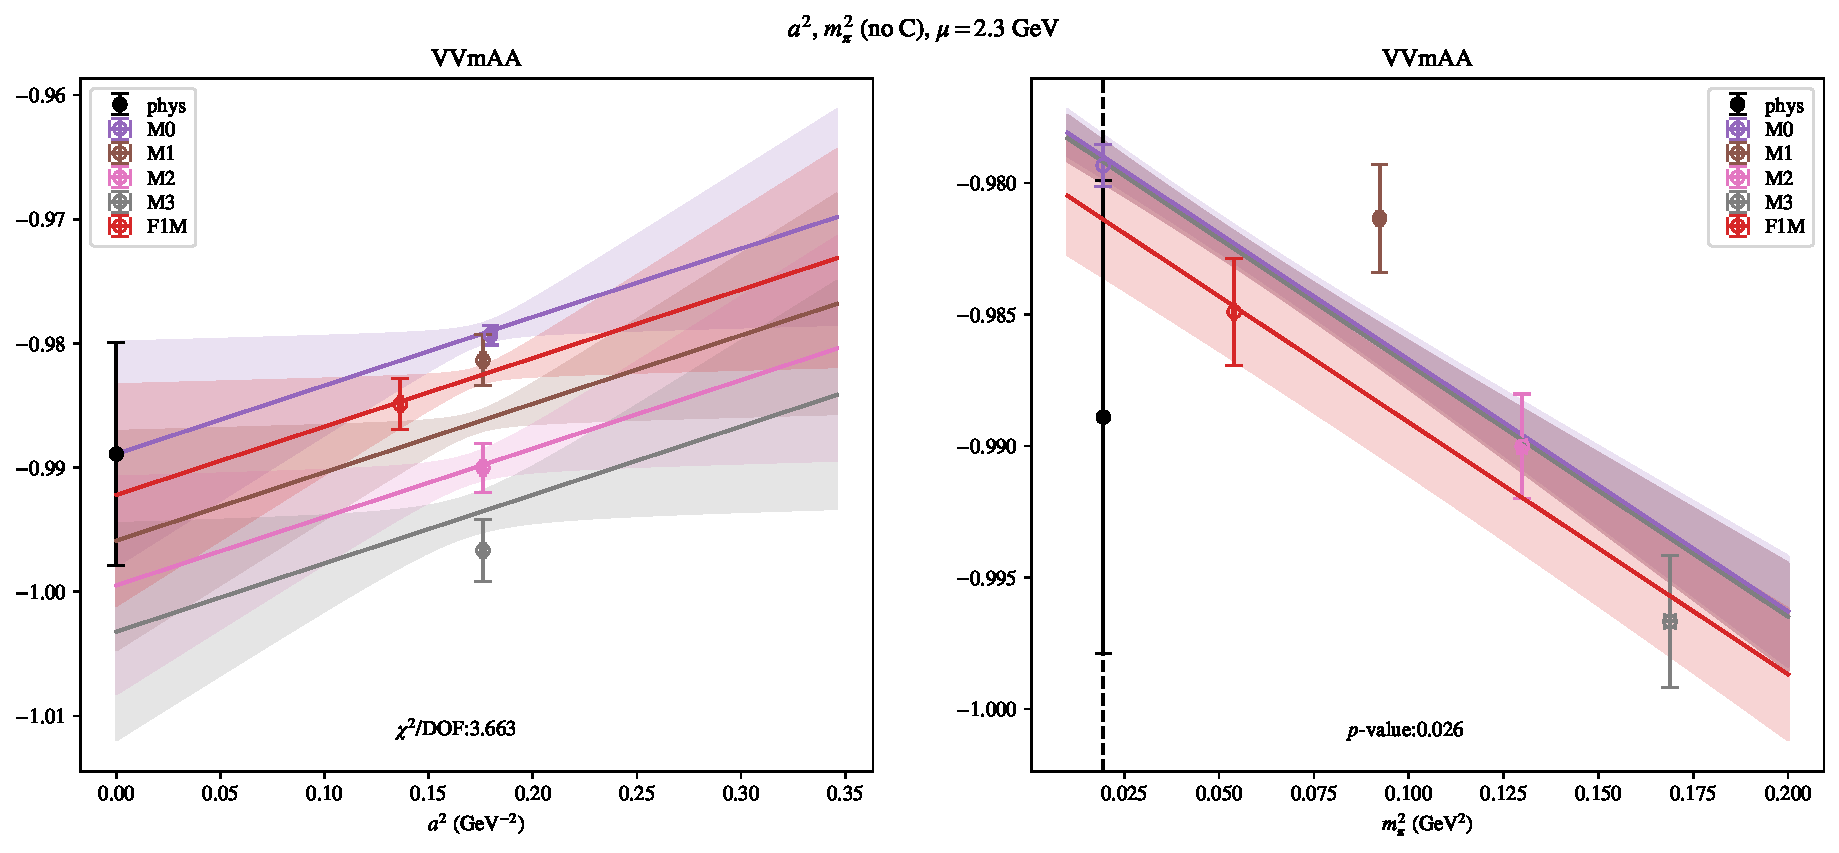
\includepdf[link, pages=-]{VVmAA/NPR/a2m2noC_23.pdf}
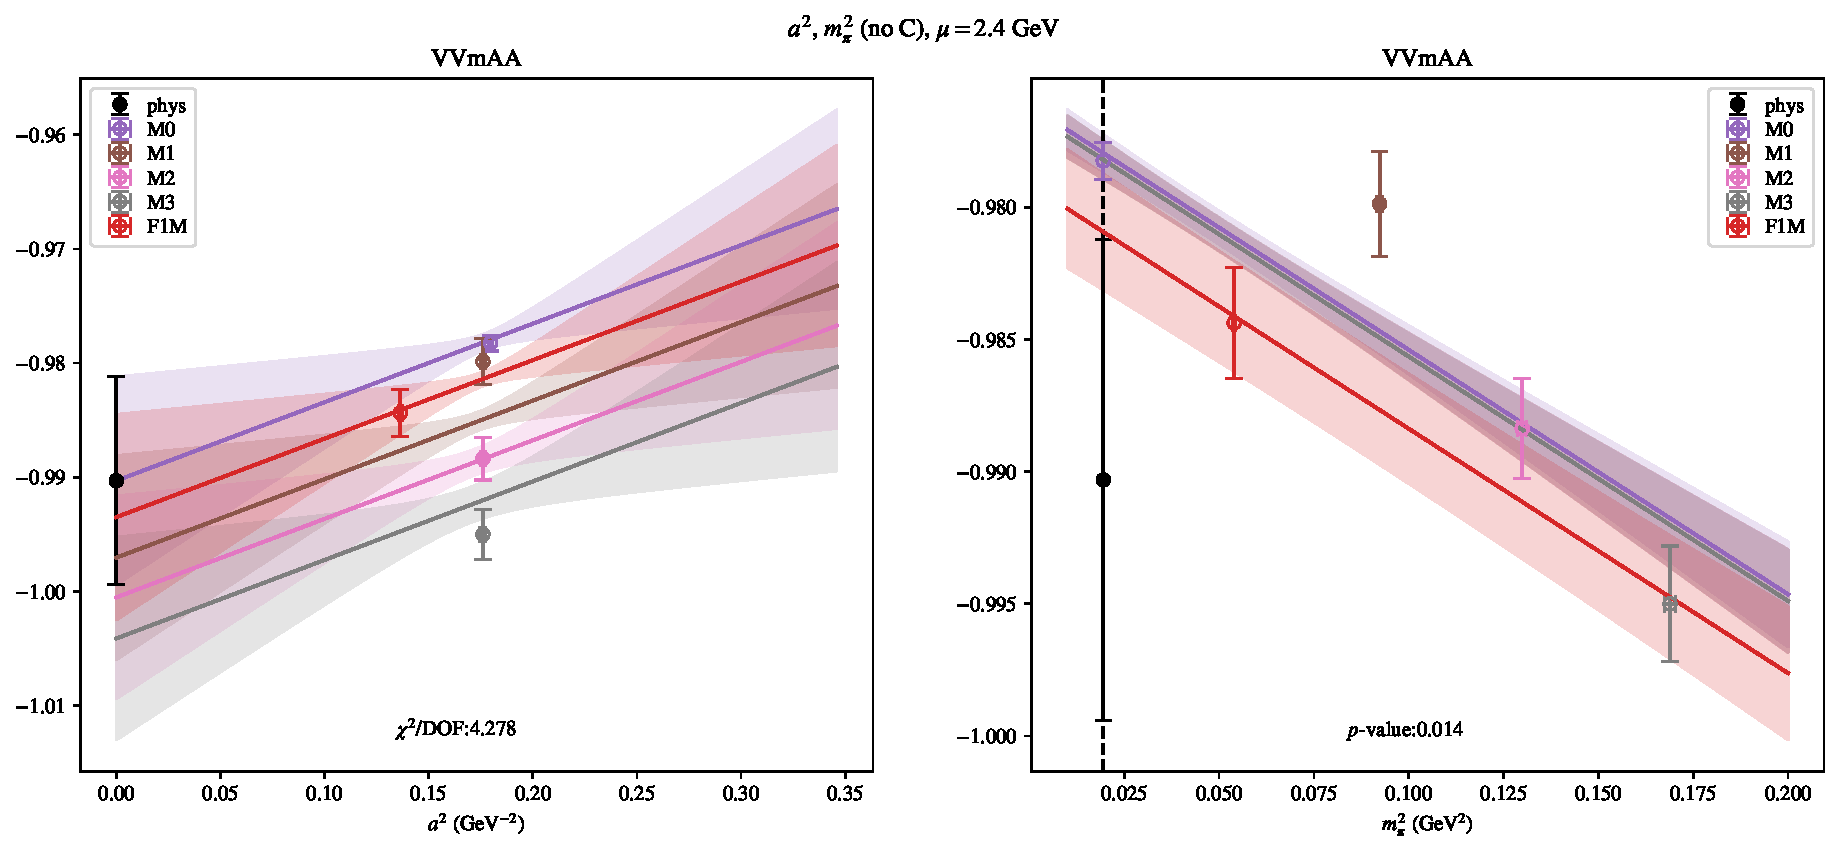
\includepdf[link, pages=-]{VVmAA/NPR/a2m2noC_24.pdf}
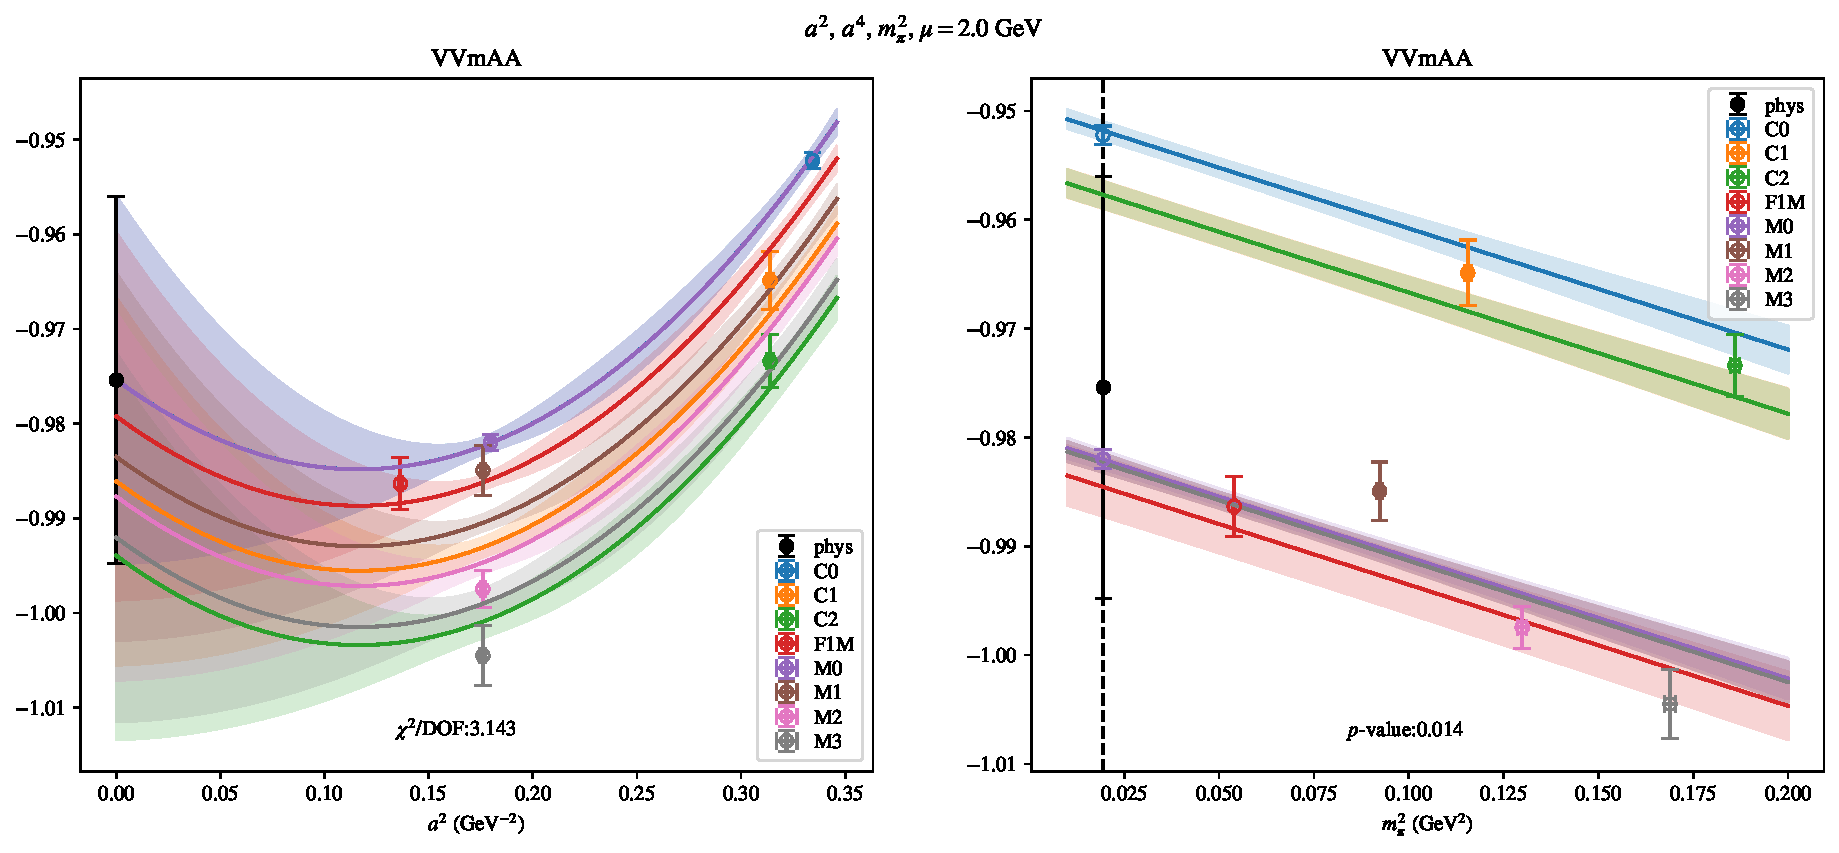
\includepdf[link, pages=-]{VVmAA/NPR/a2a4m2_20.pdf}
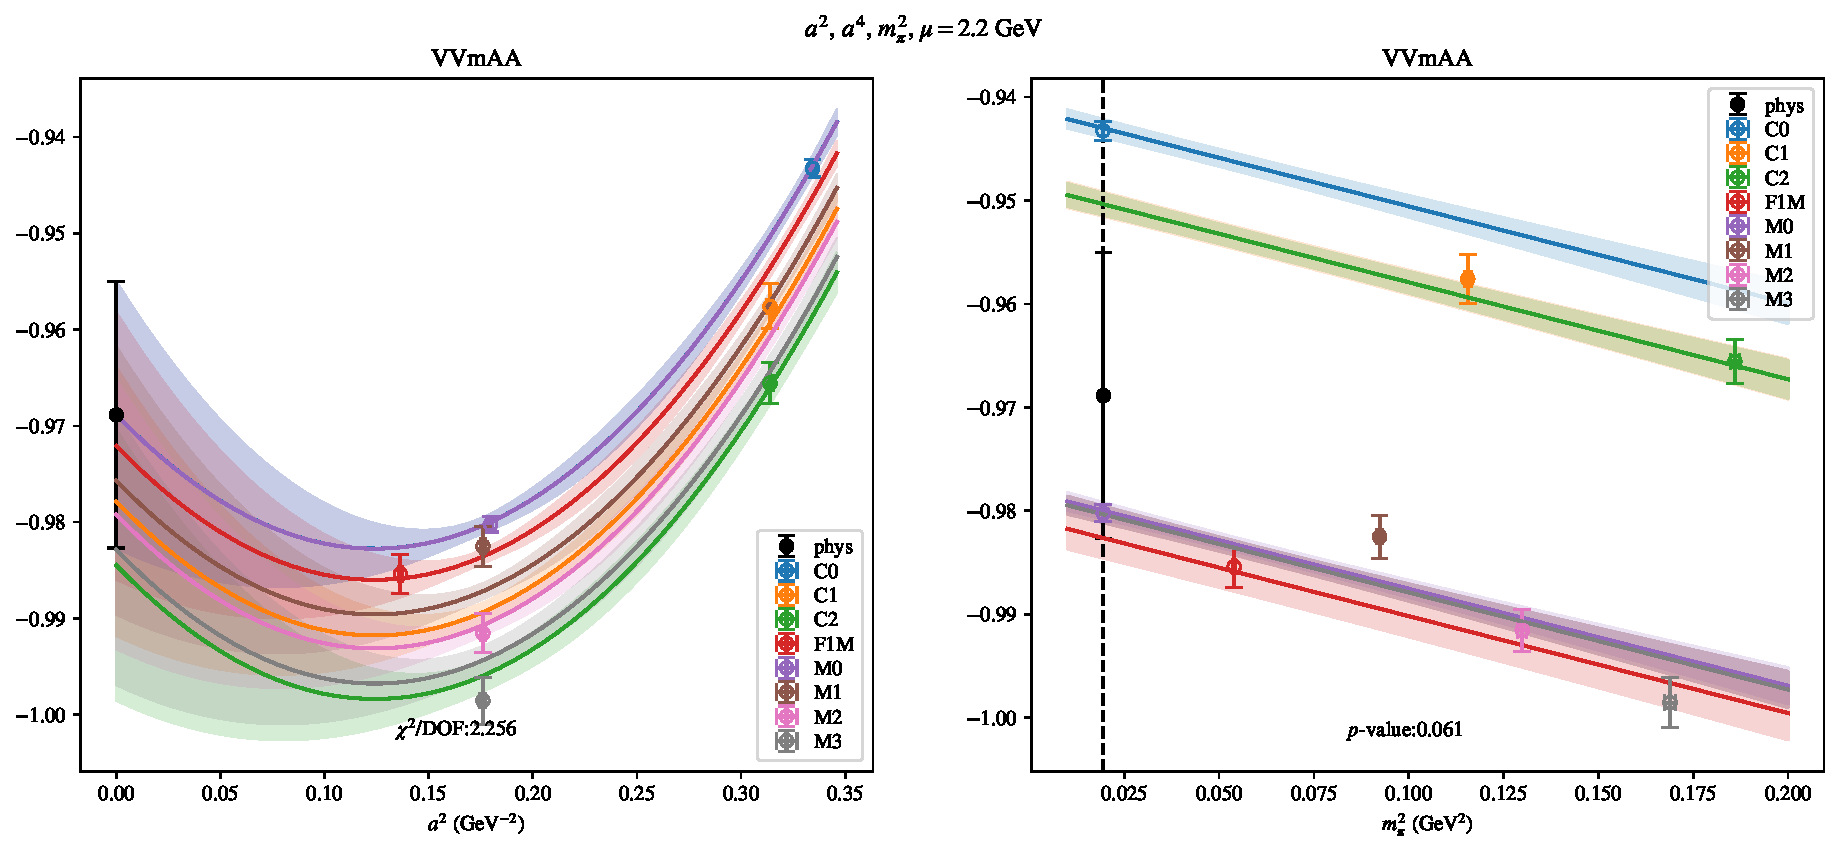
\includepdf[link, pages=-]{VVmAA/NPR/a2a4m2_22.pdf}
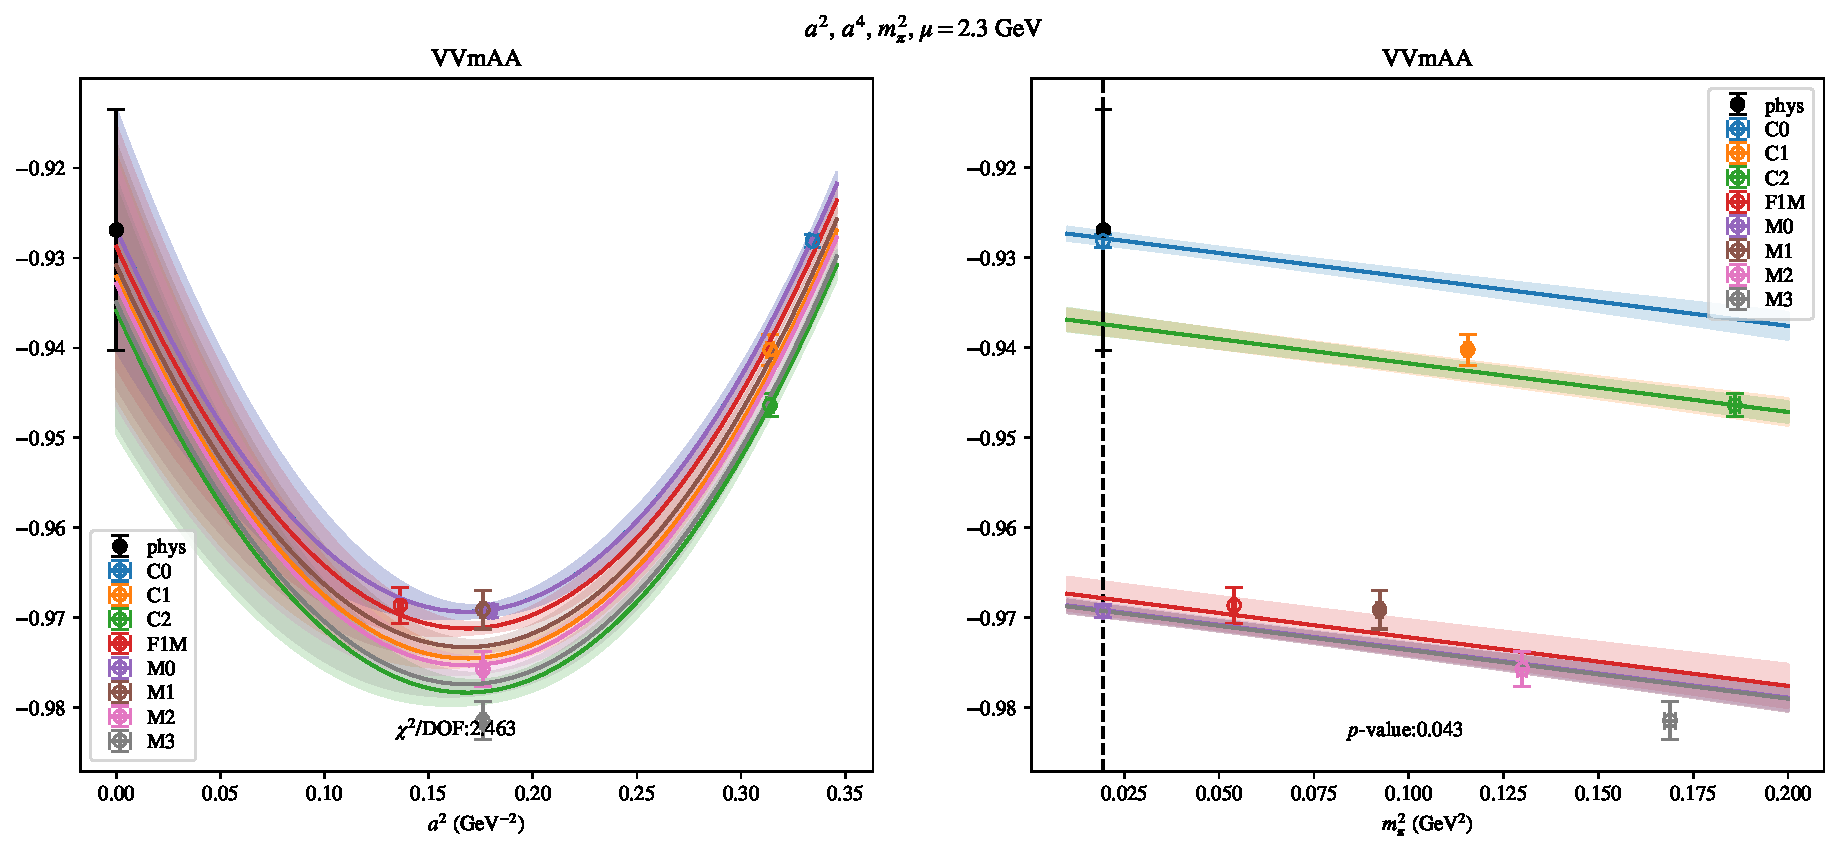
\includepdf[link, pages=-]{VVmAA/NPR/a2a4m2_23.pdf}
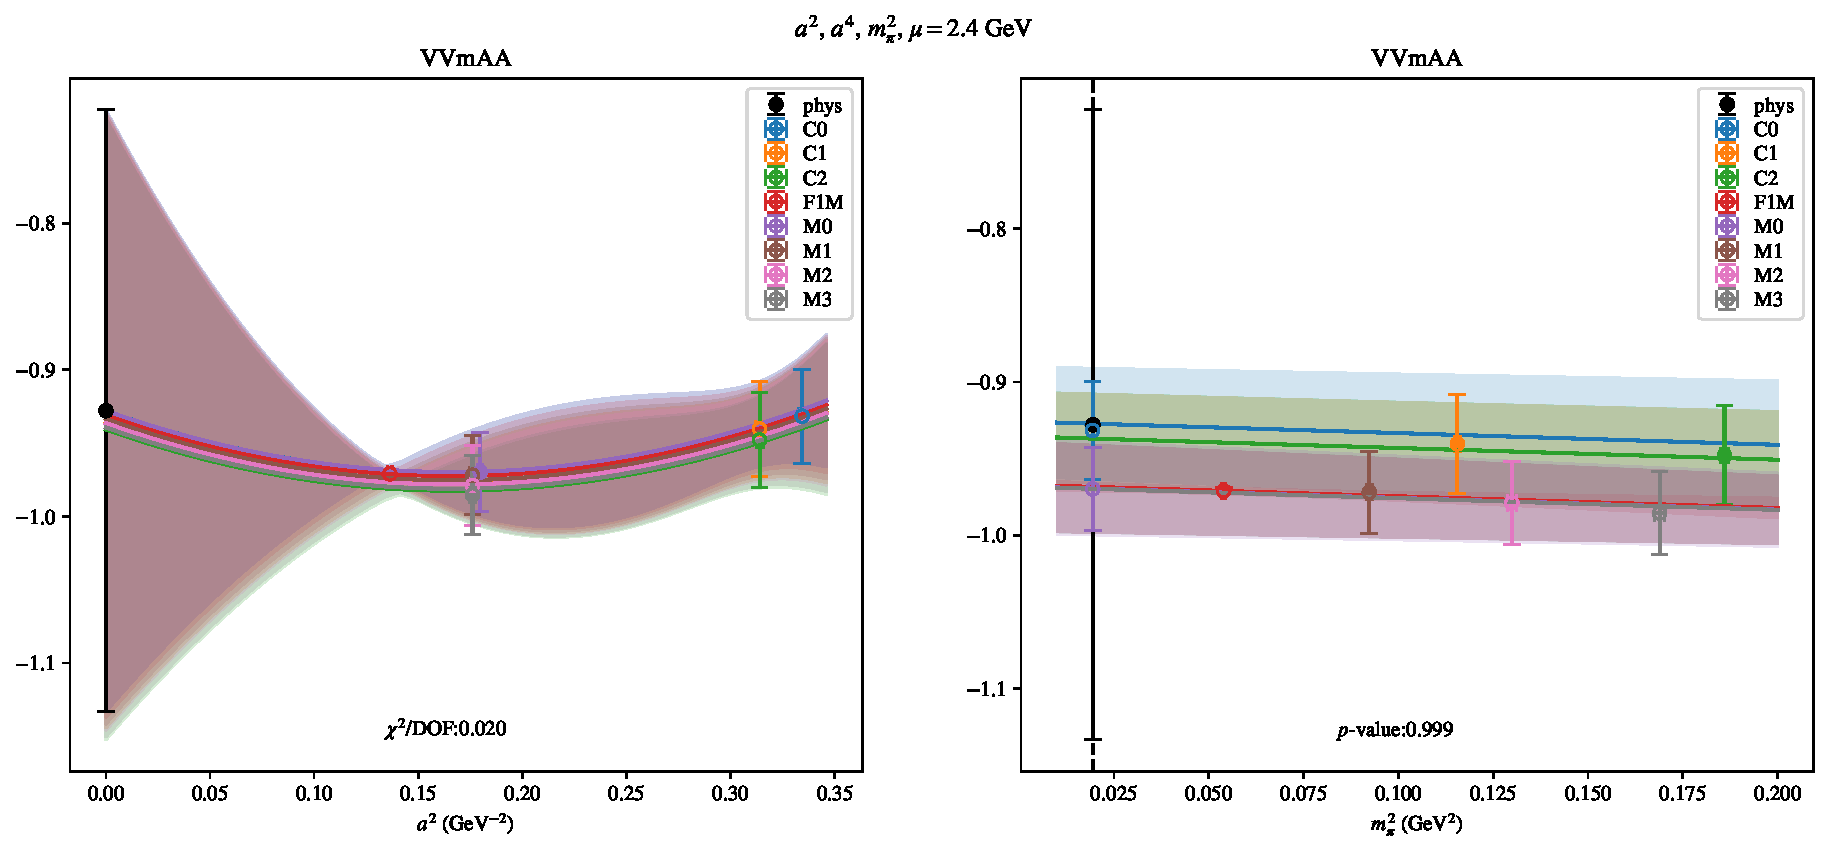
\includepdf[link, pages=-]{VVmAA/NPR/a2a4m2_24.pdf}
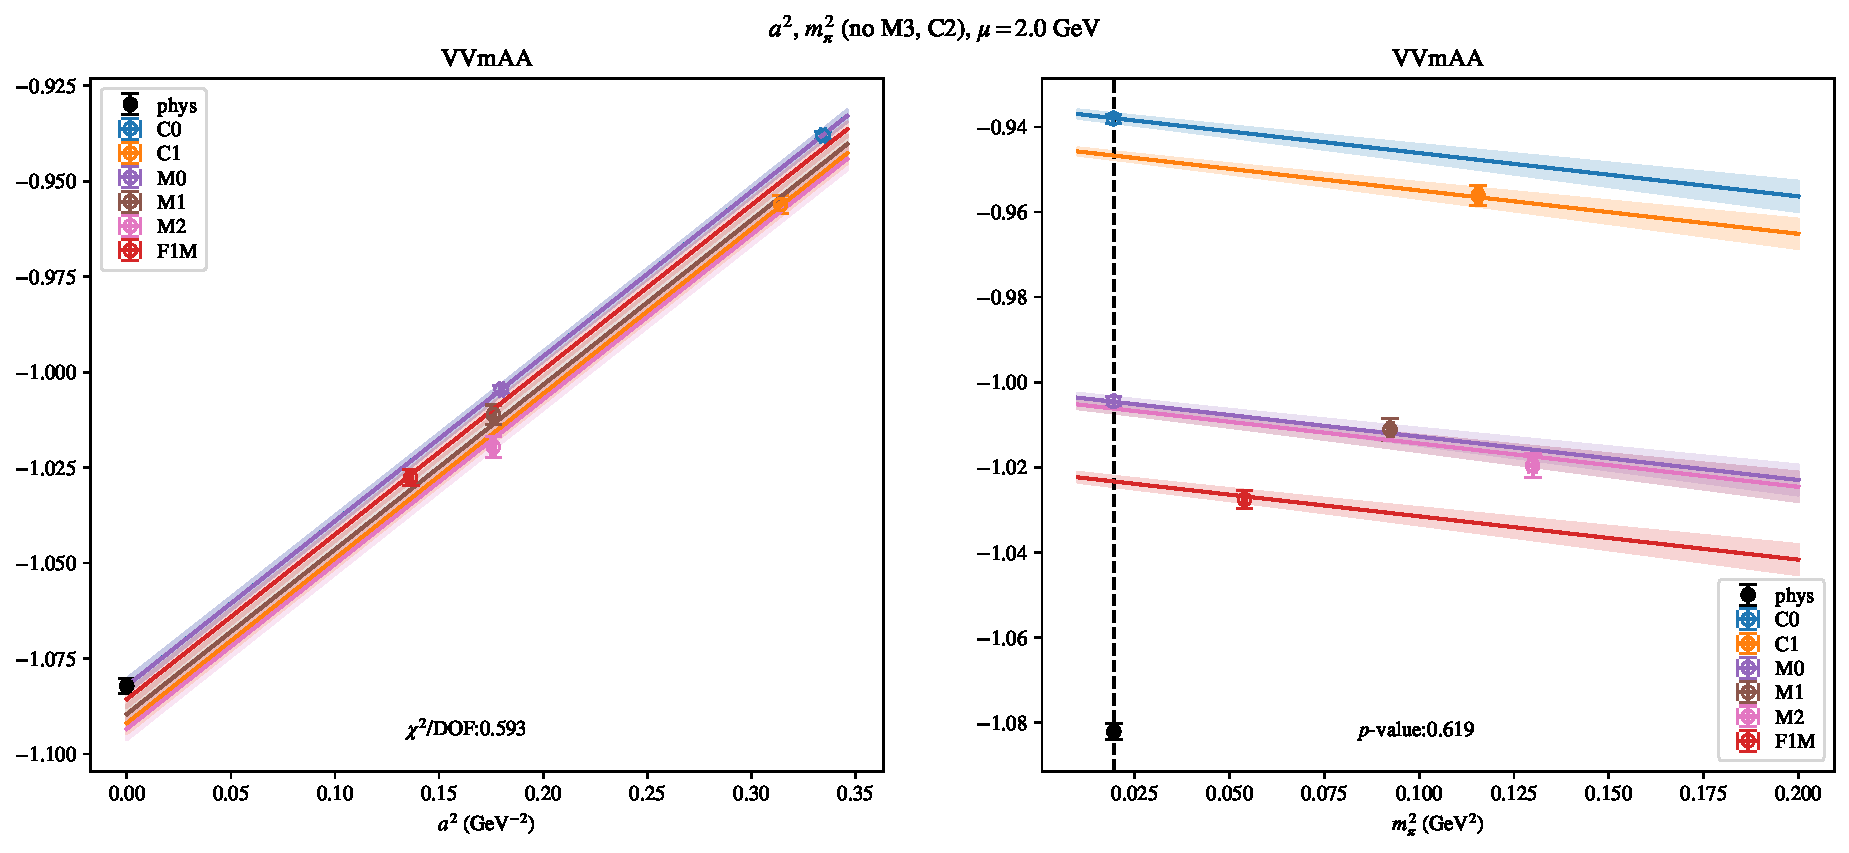
\includepdf[link, pages=-]{VVmAA/NPR/a2m2mcut_20.pdf}
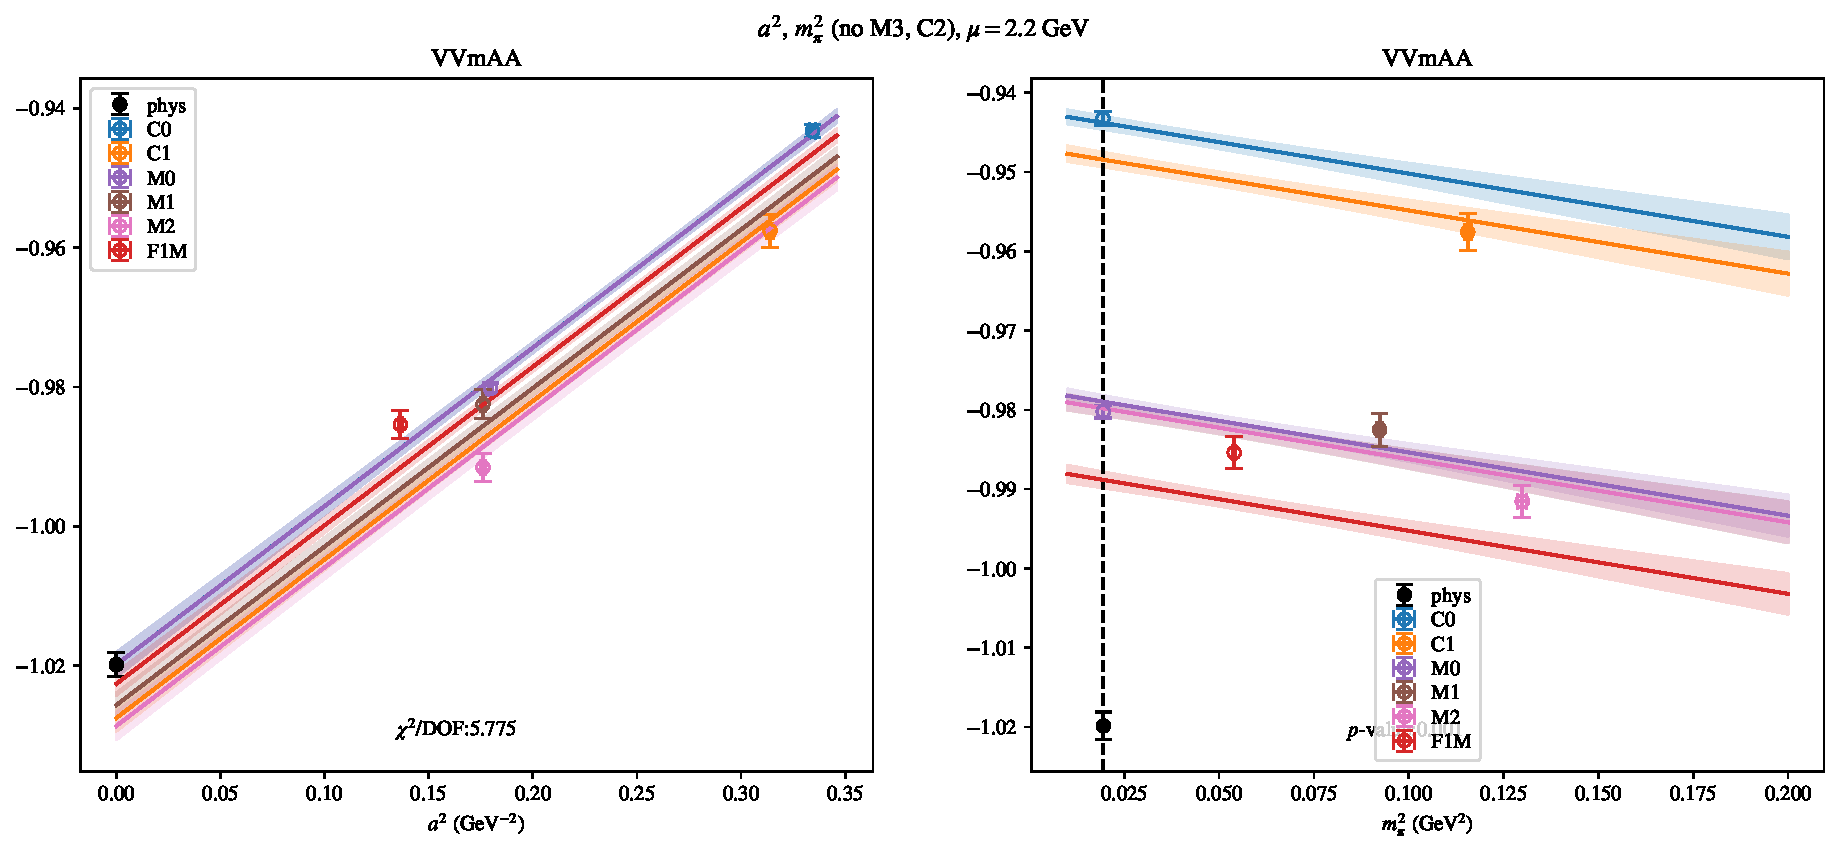
\includepdf[link, pages=-]{VVmAA/NPR/a2m2mcut_22.pdf}
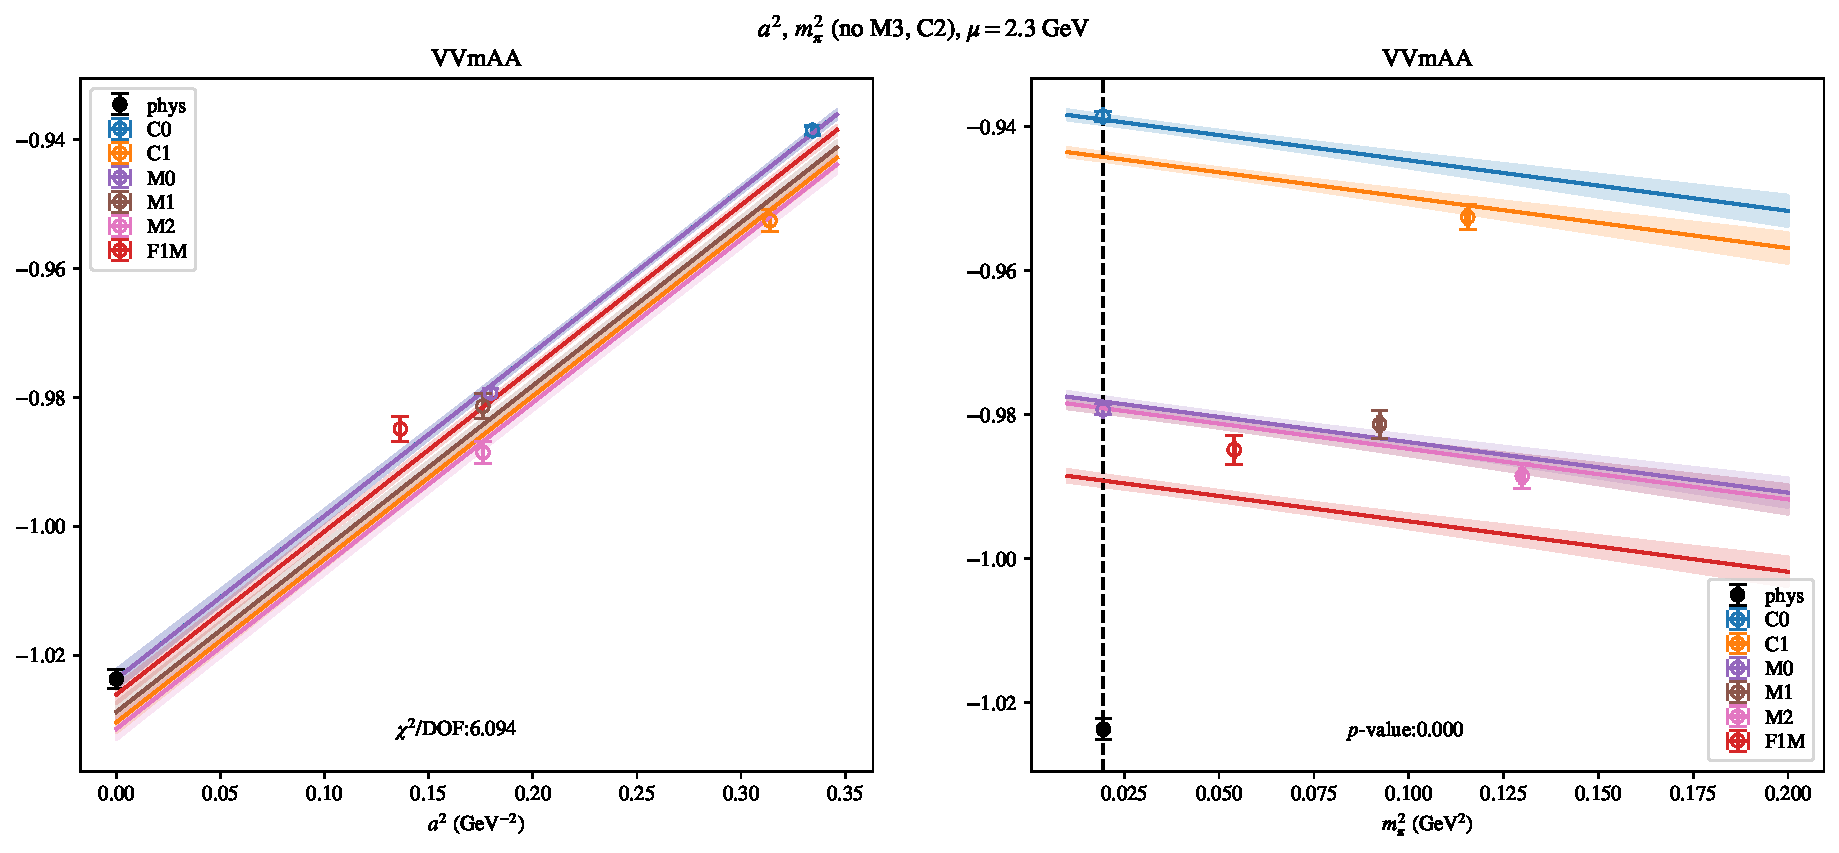
\includepdf[link, pages=-]{VVmAA/NPR/a2m2mcut_23.pdf}
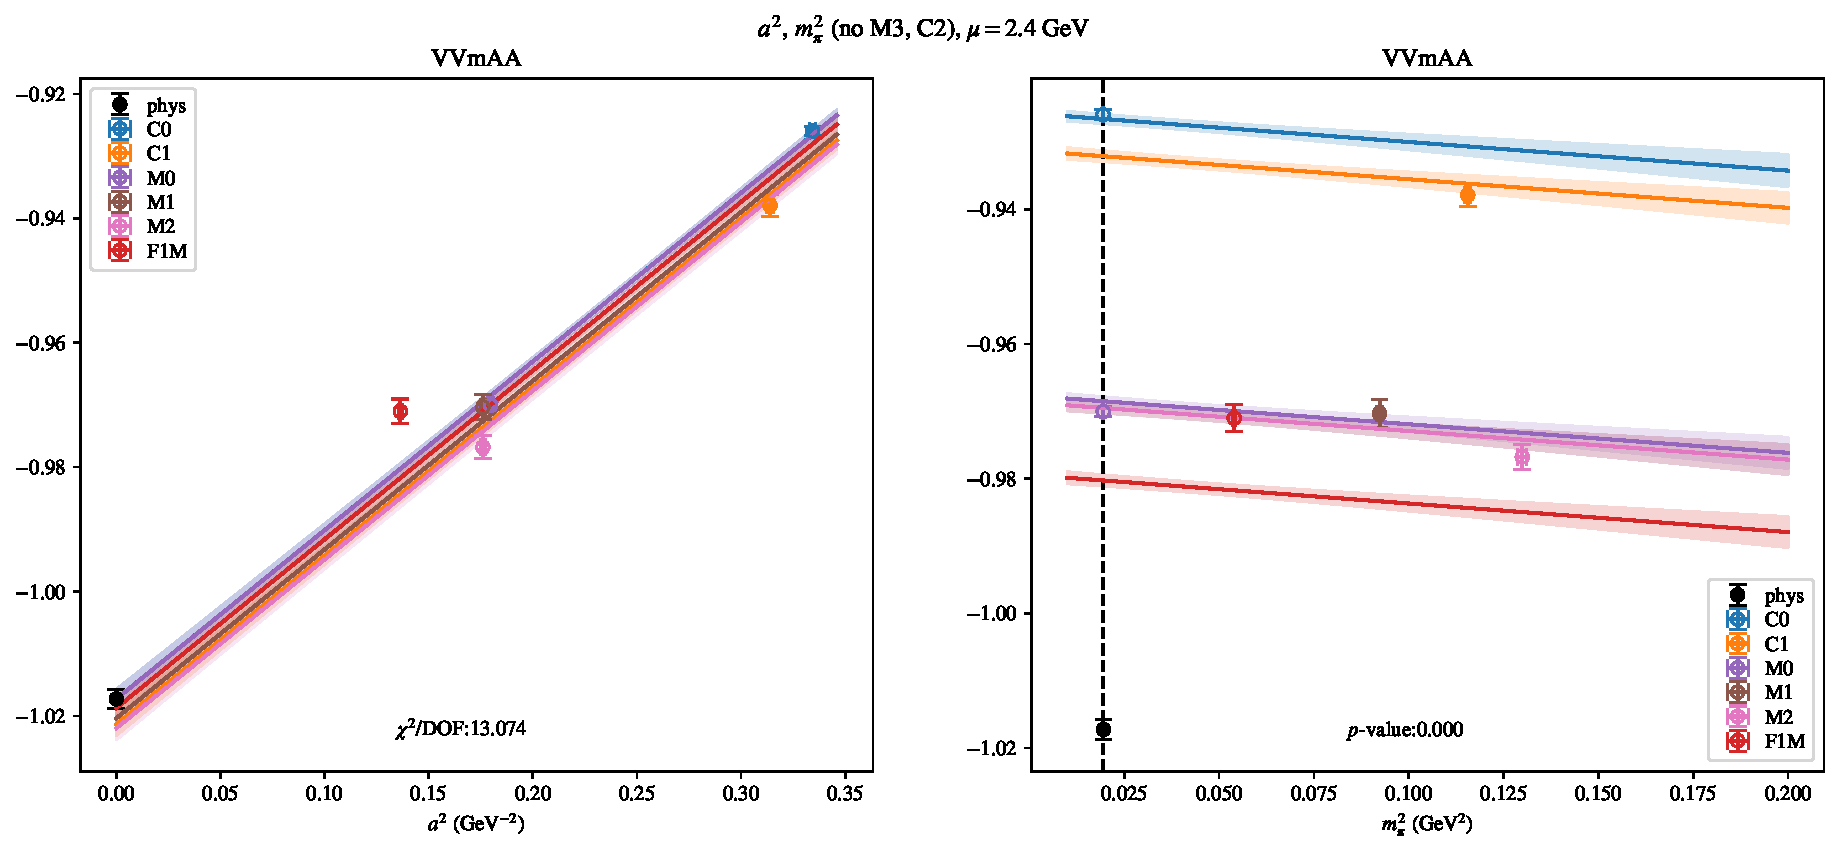
\includepdf[link, pages=-]{VVmAA/NPR/a2m2mcut_24.pdf}
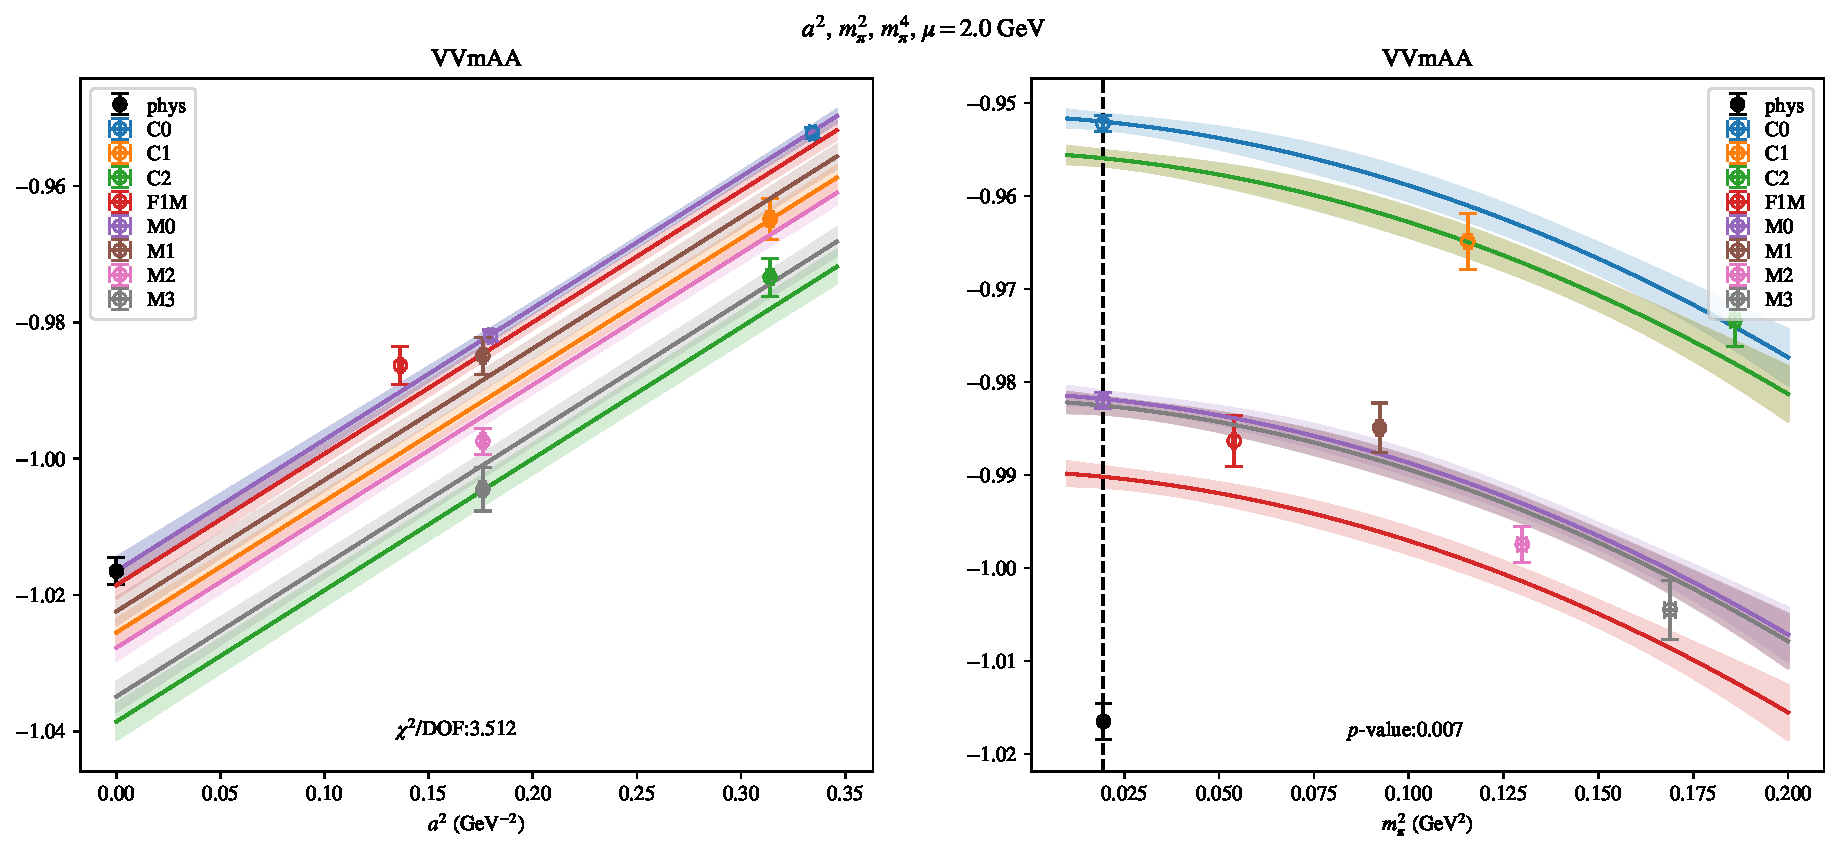
\includepdf[link, pages=-]{VVmAA/NPR/a2m2m4_20.pdf}
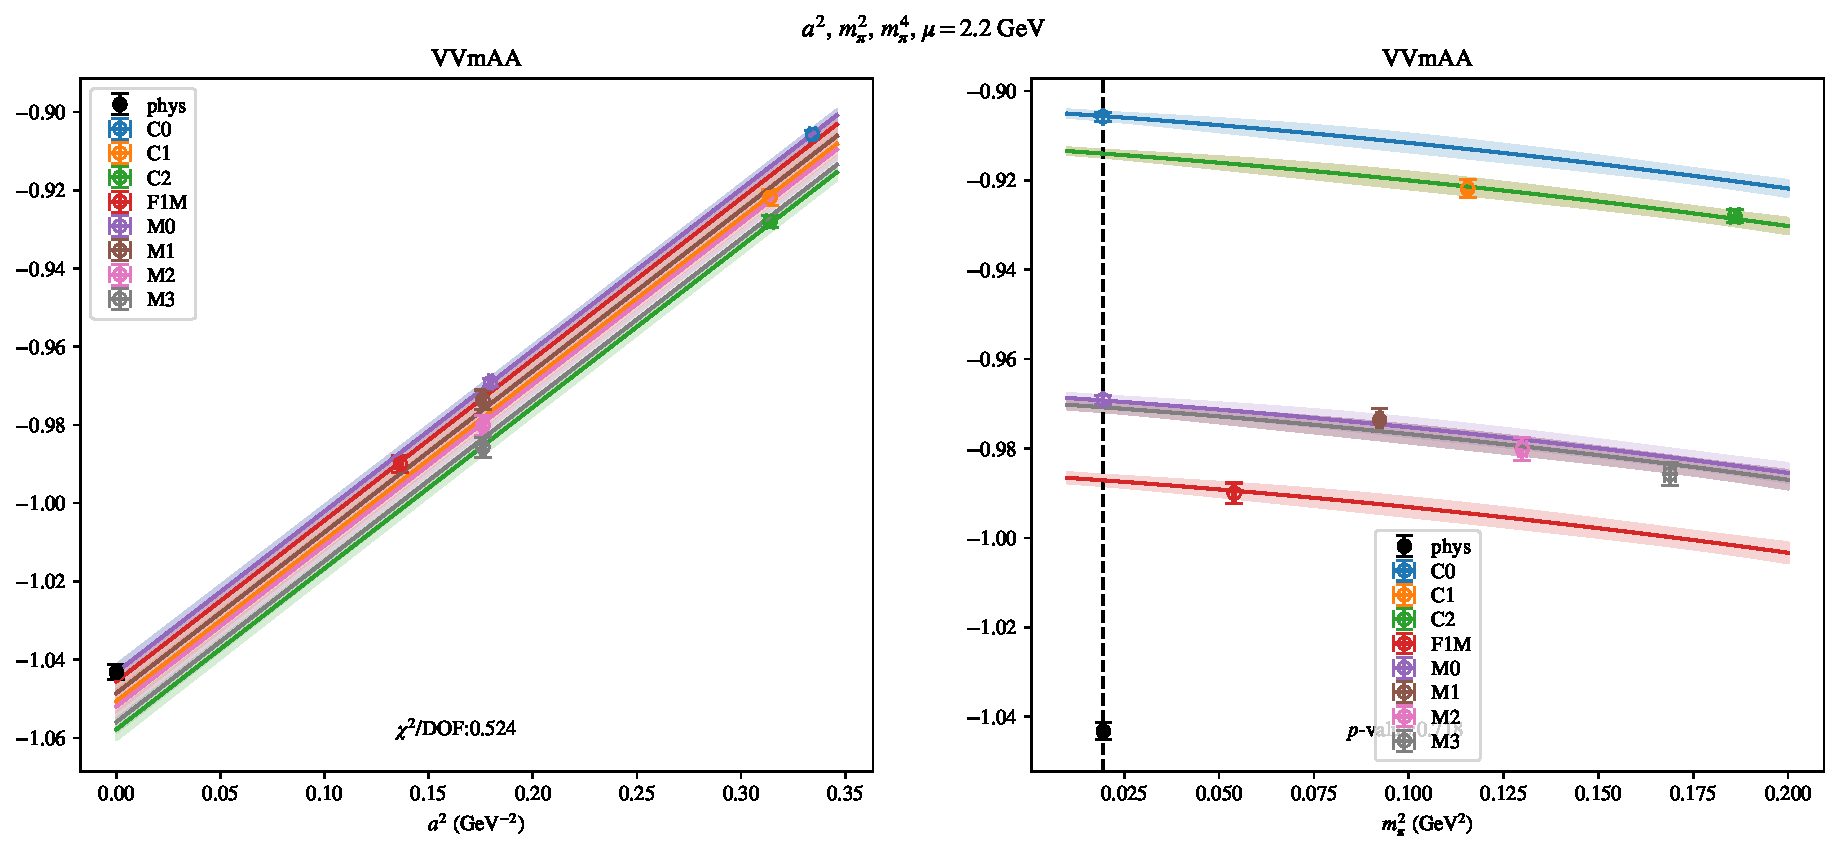
\includepdf[link, pages=-]{VVmAA/NPR/a2m2m4_22.pdf}
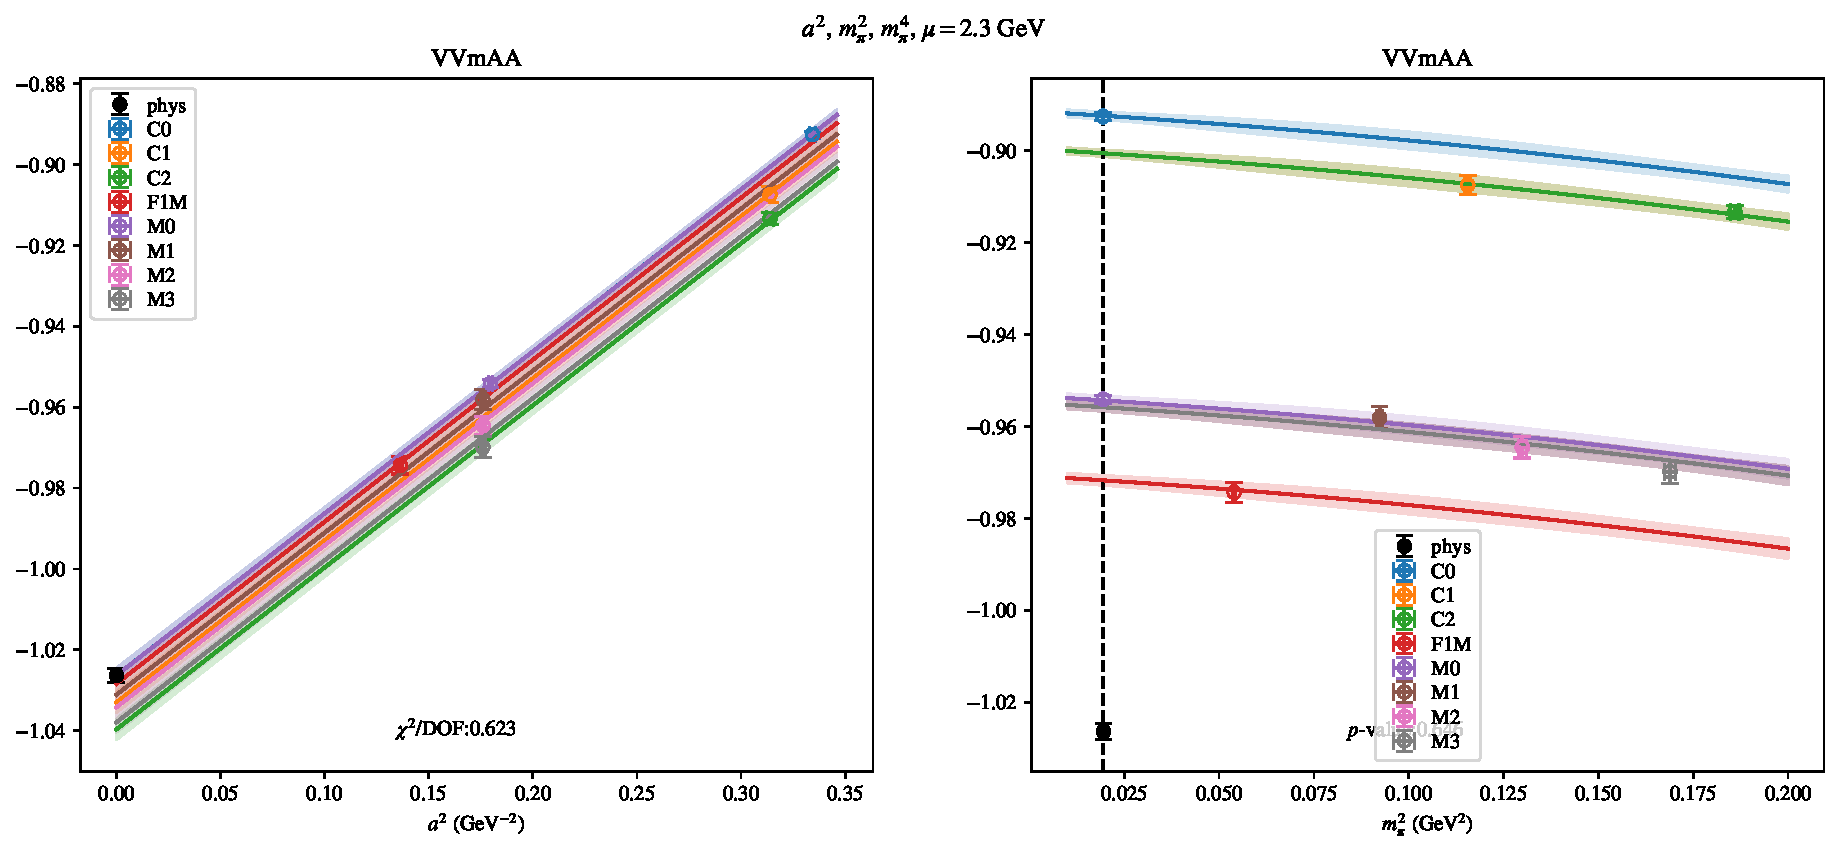
\includepdf[link, pages=-]{VVmAA/NPR/a2m2m4_23.pdf}
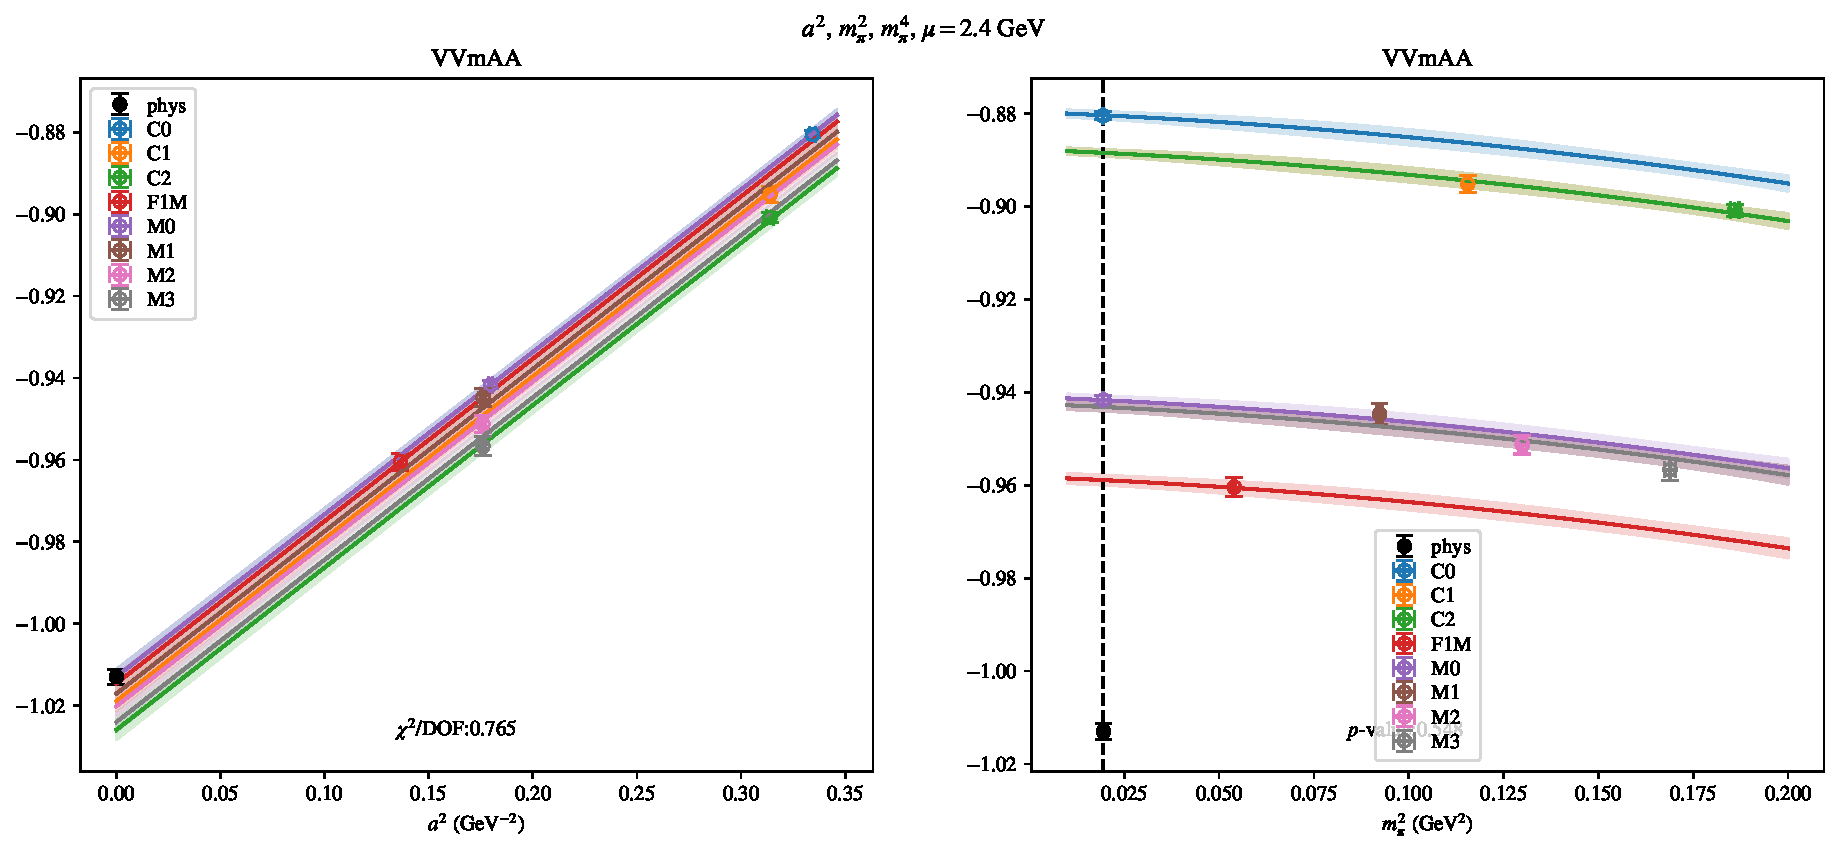
\includepdf[link, pages=-]{VVmAA/NPR/a2m2m4_24.pdf}
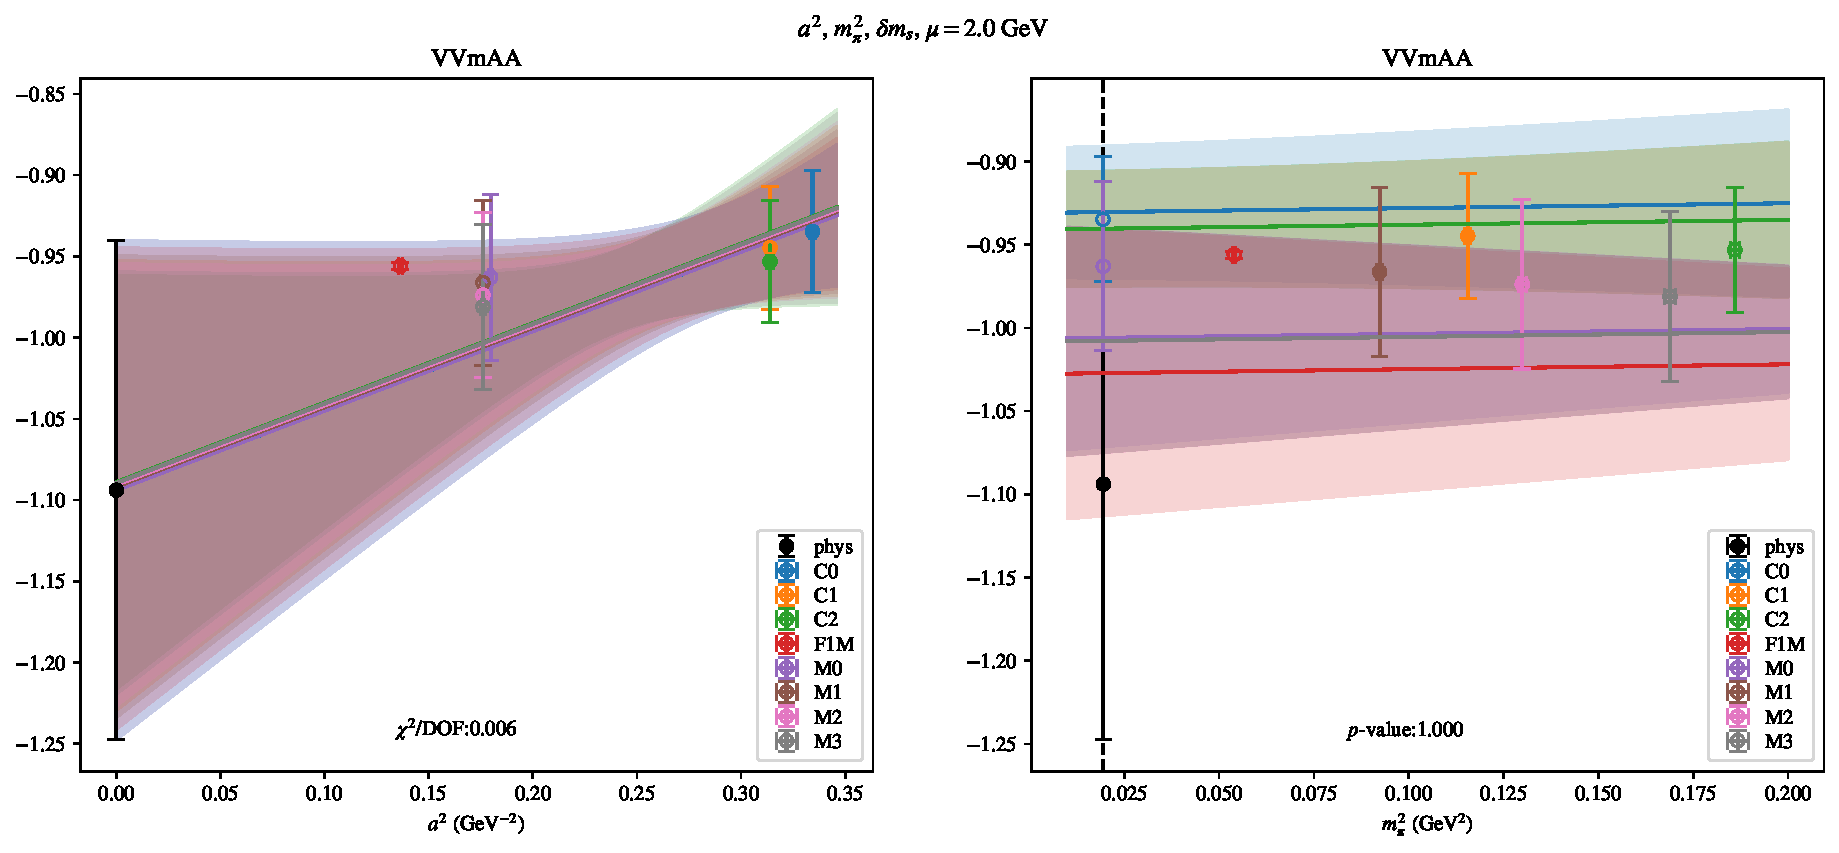
\includepdf[link, pages=-]{VVmAA/NPR/a2m2delm_20.pdf}
\includepdf[link, pages=-]{VVmAA/NPR/a2m2delm_22.pdf}
\includepdf[link, pages=-]{VVmAA/NPR/a2m2delm_23.pdf}
\includepdf[link, pages=-]{VVmAA/NPR/a2m2delm_24.pdf}
\clearpage
\section{$\mathcal{B}_3$}
\begin{table}[h!]
\begin{center}
\begin{tabular}{|c|c|c|c|c|c|c|}
\hline
$\mu$ (GeV) & $a^2$, $m_\pi^2$& $a^2$, $m_\pi^2$ (no C)& $a^2$, $a^4$, $m_\pi^2$& $a^2$, $m_\pi^2$ (no M3, C2)& $a^2$, $m_\pi^2$, $m_\pi^4$& $a^2$, $m_\pi^2$, $\delta m_s$\\
\hline
2.0& \hyperlink{SSmPP/NPR/a2m2_20.pdf.1}{\textbf{1.8001(27)}: 16.176 (0.0)} & \hyperlink{SSmPP/NPR/a2m2noC_20.pdf.1}{\textbf{1.692(13)}: 0.632 (0.532)} & \hyperlink{SSmPP/NPR/a2a4m2_20.pdf.1}{\textbf{1.622(20)}: 1.008 (0.402)} & \hyperlink{SSmPP/NPR/a2m2mcut_20.pdf.1}{\textbf{1.8014(28)}: 25.461 (0.0)} & \hyperlink{SSmPP/NPR/a2m2m4_20.pdf.1}{\textbf{1.8052(28)}: 15.552 (0.0)} & \hyperlink{SSmPP/NPR/a2m2delm_20.pdf.1}{\textbf{1.8111(30)}: 1.39 (0.235)}\\
2.2& \hyperlink{SSmPP/NPR/a2m2_22.pdf.1}{\textbf{1.8056(26)}: 14.919 (0.0)} & \hyperlink{SSmPP/NPR/a2m2noC_22.pdf.1}{\textbf{1.705(12)}: 1.332 (0.264)} & \hyperlink{SSmPP/NPR/a2a4m2_22.pdf.1}{\textbf{1.639(20)}: 1.476 (0.207)} & \hyperlink{SSmPP/NPR/a2m2mcut_22.pdf.1}{\textbf{1.8070(27)}: 22.411 (0.0)} & \hyperlink{SSmPP/NPR/a2m2m4_22.pdf.1}{\textbf{1.8108(27)}: 13.495 (0.0)} & \hyperlink{SSmPP/NPR/a2m2delm_22.pdf.1}{\textbf{1.8156(28)}: 2.276 (0.059)}\\
2.3& \hyperlink{SSmPP/NPR/a2m2_23.pdf.1}{\textbf{1.8080(25)}: 14.291 (0.0)} & \hyperlink{SSmPP/NPR/a2m2noC_23.pdf.1}{\textbf{1.709(12)}: 1.494 (0.224)} & \hyperlink{SSmPP/NPR/a2a4m2_23.pdf.1}{\textbf{1.644(20)}: 1.377 (0.239)} & \hyperlink{SSmPP/NPR/a2m2mcut_23.pdf.1}{\textbf{1.8093(27)}: 21.689 (0.0)} & \hyperlink{SSmPP/NPR/a2m2m4_23.pdf.1}{\textbf{1.8130(27)}: 13.268 (0.0)} & \hyperlink{SSmPP/NPR/a2m2delm_23.pdf.1}{\textbf{1.8174(28)}: 2.378 (0.05)}\\
2.4& \hyperlink{SSmPP/NPR/a2m2_24.pdf.1}{\textbf{1.8094(25)}: 13.225 (0.0)} & \hyperlink{SSmPP/NPR/a2m2noC_24.pdf.1}{\textbf{1.714(12)}: 1.506 (0.222)} & \hyperlink{SSmPP/NPR/a2a4m2_24.pdf.1}{\textbf{1.652(20)}: 1.367 (0.243)} & \hyperlink{SSmPP/NPR/a2m2mcut_24.pdf.1}{\textbf{1.8106(27)}: 20.205 (0.0)} & \hyperlink{SSmPP/NPR/a2m2m4_24.pdf.1}{\textbf{1.8142(27)}: 12.492 (0.0)} & \hyperlink{SSmPP/NPR/a2m2delm_24.pdf.1}{\textbf{1.8182(27)}: 2.29 (0.057)}\\
\hline
\end{tabular}
\caption{Physical point value from chiral and continuum extrapolation at renormalisation scale $\mu$. Entries are \textbf{value(error)}: $\chi^2/\text{DOF}$ ($p$-value).}
\end{center}
\end{table}
\begin{table}[h!]
\begin{center}
\begin{tabular}{|c c|c|c|c|c|c|c|}
\hline
$\mu$ (GeV) &  & $a^2$, $m_\pi^2$& $a^2$, $m_\pi^2$ (no C)& $a^2$, $a^4$, $m_\pi^2$& $a^2$, $m_\pi^2$ (no M3, C2)& $a^2$, $m_\pi^2$, $m_\pi^4$& $a^2$, $m_\pi^2$, $\delta m_s$\\
\hline
\multirow{2}{0.5in}{2.0} & $\alpha$ & 0.0704(58)& 0.446(47)& 1.06(12)& 0.0683(60)& 0.0610(61)& 0.0496(62)\\
 & $\beta$ & -0.0010(13)& -0.0011(26)& -0.0015(15)& -0.0015(24)& -0.0041(70)& -0.0013(13)\\
\hline
\multirow{2}{0.5in}{2.2} & $\alpha$ & 0.0761(55)& 0.425(46)& 0.99(12)& 0.0739(58)& 0.0667(58)& 0.0573(59)\\
 & $\beta$ & -0.0007(12)& -0.0008(23)& -0.0011(14)& -0.0012(23)& -0.0037(65)& -0.0009(12)\\
\hline
\multirow{2}{0.5in}{2.3} & $\alpha$ & 0.0772(54)& 0.417(46)& 0.97(12)& 0.0752(57)& 0.0681(57)& 0.0595(58)\\
 & $\beta$ & -0.0007(11)& -0.0008(22)& -0.0011(14)& -0.0011(22)& -0.0034(64)& -0.0009(11)\\
\hline
\multirow{2}{0.5in}{2.4} & $\alpha$ & 0.0790(54)& 0.406(45)& 0.93(12)& 0.0771(58)& 0.0702(57)& 0.0625(57)\\
 & $\beta$ & -0.0006(11)& -0.0007(21)& -0.0010(13)& -0.0010(21)& -0.0032(63)& -0.0008(11)\\
\hline
\end{tabular}
\caption{Fit values of coefficients in $Q = Q_{phys} + \mathbf{\alpha} a^2 + \mathbf{\beta}\left(\frac{m_\pi^2}{f_\pi^2}-\frac{m_{\pi,PDG}^2}{f_\pi^2}\right) + \ldots$.}
\end{center}
\end{table}
\includepdf[link, pages=-]{SSmPP/NPR/a2m2_20.pdf}
\includepdf[link, pages=-]{SSmPP/NPR/a2m2_22.pdf}
\includepdf[link, pages=-]{SSmPP/NPR/a2m2_23.pdf}
\includepdf[link, pages=-]{SSmPP/NPR/a2m2_24.pdf}
\includepdf[link, pages=-]{SSmPP/NPR/a2m2noC_20.pdf}
\includepdf[link, pages=-]{SSmPP/NPR/a2m2noC_22.pdf}
\includepdf[link, pages=-]{SSmPP/NPR/a2m2noC_23.pdf}
\includepdf[link, pages=-]{SSmPP/NPR/a2m2noC_24.pdf}
\includepdf[link, pages=-]{SSmPP/NPR/a2a4m2_20.pdf}
\includepdf[link, pages=-]{SSmPP/NPR/a2a4m2_22.pdf}
\includepdf[link, pages=-]{SSmPP/NPR/a2a4m2_23.pdf}
\includepdf[link, pages=-]{SSmPP/NPR/a2a4m2_24.pdf}
\includepdf[link, pages=-]{SSmPP/NPR/a2m2mcut_20.pdf}
\includepdf[link, pages=-]{SSmPP/NPR/a2m2mcut_22.pdf}
\includepdf[link, pages=-]{SSmPP/NPR/a2m2mcut_23.pdf}
\includepdf[link, pages=-]{SSmPP/NPR/a2m2mcut_24.pdf}
\includepdf[link, pages=-]{SSmPP/NPR/a2m2m4_20.pdf}
\includepdf[link, pages=-]{SSmPP/NPR/a2m2m4_22.pdf}
\includepdf[link, pages=-]{SSmPP/NPR/a2m2m4_23.pdf}
\includepdf[link, pages=-]{SSmPP/NPR/a2m2m4_24.pdf}
\includepdf[link, pages=-]{SSmPP/NPR/a2m2delm_20.pdf}
\includepdf[link, pages=-]{SSmPP/NPR/a2m2delm_22.pdf}
\includepdf[link, pages=-]{SSmPP/NPR/a2m2delm_23.pdf}
\includepdf[link, pages=-]{SSmPP/NPR/a2m2delm_24.pdf}
\clearpage
\section{$\mathcal{B}_4$}
\begin{table}[h!]
\begin{center}
\begin{tabular}{|c|c|c|c|c|c|c|}
\hline
$\mu$ (GeV) & $a^2$, $m_\pi^2$& $a^2$, $m_\pi^2$ (no C)& $a^2$, $a^4$, $m_\pi^2$& $a^2$, $m_\pi^2$ (no M3, C2)& $a^2$, $m_\pi^2$, $m_\pi^4$& $a^2$, $m_\pi^2$, $\delta m_s$\\
\hline
2.0& \hyperlink{SSpPP/NPR/a2m2_20.pdf.1}{\textbf{-0.925(17)}: 2.894 (0.013)} & \hyperlink{SSpPP/NPR/a2m2noC_20.pdf.1}{\textbf{-0.93(10)}: 2.443 (0.087)} & \hyperlink{SSpPP/NPR/a2a4m2_20.pdf.1}{\textbf{-0.92(16)}: 3.616 (0.006)} & \hyperlink{SSpPP/NPR/a2m2mcut_20.pdf.1}{\textbf{-0.925(19)}: 3.175 (0.023)} & \hyperlink{SSpPP/NPR/a2m2m4_20.pdf.1}{\textbf{-0.924(19)}: 2.62 (0.033)} & \hyperlink{SSpPP/NPR/a2m2delm_20.pdf.1}{\textbf{-0.925(18)}: 3.511 (0.007)}\\
2.2& \hyperlink{SSpPP/NPR/a2m2_22.pdf.1}{\textbf{-0.905(16)}: 3.98 (0.001)} & \hyperlink{SSpPP/NPR/a2m2noC_22.pdf.1}{\textbf{-0.920(95)}: 2.011 (0.134)} & \hyperlink{SSpPP/NPR/a2a4m2_22.pdf.1}{\textbf{-0.90(16)}: 4.973 (0.001)} & \hyperlink{SSpPP/NPR/a2m2mcut_22.pdf.1}{\textbf{-0.906(19)}: 4.236 (0.005)} & \hyperlink{SSpPP/NPR/a2m2m4_22.pdf.1}{\textbf{-0.904(19)}: 4.225 (0.002)} & \hyperlink{SSpPP/NPR/a2m2delm_22.pdf.1}{\textbf{-0.905(18)}: 4.624 (0.001)}\\
2.3& \hyperlink{SSpPP/NPR/a2m2_23.pdf.1}{\textbf{-0.897(16)}: 4.447 (0.0)} & \hyperlink{SSpPP/NPR/a2m2noC_23.pdf.1}{\textbf{-0.913(94)}: 2.279 (0.102)} & \hyperlink{SSpPP/NPR/a2a4m2_23.pdf.1}{\textbf{-0.89(15)}: 5.557 (0.0)} & \hyperlink{SSpPP/NPR/a2m2mcut_23.pdf.1}{\textbf{-0.897(18)}: 4.907 (0.002)} & \hyperlink{SSpPP/NPR/a2m2m4_23.pdf.1}{\textbf{-0.895(19)}: 4.634 (0.001)} & \hyperlink{SSpPP/NPR/a2m2delm_23.pdf.1}{\textbf{-0.896(18)}: 5.079 (0.0)}\\
2.4& \hyperlink{SSpPP/NPR/a2m2_24.pdf.1}{\textbf{-0.889(16)}: 4.844 (0.0)} & \hyperlink{SSpPP/NPR/a2m2noC_24.pdf.1}{\textbf{-0.906(93)}: 2.406 (0.09)} & \hyperlink{SSpPP/NPR/a2a4m2_24.pdf.1}{\textbf{-0.88(15)}: 6.054 (0.0)} & \hyperlink{SSpPP/NPR/a2m2mcut_24.pdf.1}{\textbf{-0.889(18)}: 5.489 (0.001)} & \hyperlink{SSpPP/NPR/a2m2m4_24.pdf.1}{\textbf{-0.888(19)}: 5.163 (0.0)} & \hyperlink{SSpPP/NPR/a2m2delm_24.pdf.1}{\textbf{-0.888(17)}: 5.538 (0.0)}\\
\hline
\end{tabular}
\caption{Physical point value from chiral and continuum extrapolation at renormalisation scale $\mu$. Entries are \textbf{value(error)}: $\chi^2/\text{DOF}$ ($p$-value).}
\end{center}
\end{table}
\begin{table}[h!]
\begin{center}
\begin{tabular}{|c c|c|c|c|c|c|c|}
\hline
$\mu$ (GeV) &  & $a^2$, $m_\pi^2$& $a^2$, $m_\pi^2$ (no C)& $a^2$, $a^4$, $m_\pi^2$& $a^2$, $m_\pi^2$ (no M3, C2)& $a^2$, $m_\pi^2$, $m_\pi^4$& $a^2$, $m_\pi^2$, $\delta m_s$\\
\hline
\multirow{2}{0.5in}{2.0} & $\alpha$ & 0.3756(79)& 0.307(66)& 0.38(17)& 0.3754(88)& 0.3810(88)& 0.3772(83)\\
 & $\beta$ & 0.00666(17)& 0.00614(28)& 0.00666(18)& 0.00704(29)& 0.00834(87)& 0.00669(18)\\
\hline
\multirow{2}{0.5in}{2.2} & $\alpha$ & 0.4230(80)& 0.329(64)& 0.43(17)& 0.4195(88)& 0.4277(88)& 0.4260(85)\\
 & $\beta$ & 0.00705(16)& 0.00635(24)& 0.00706(17)& 0.00737(27)& 0.00843(81)& 0.00711(17)\\
\hline
\multirow{2}{0.5in}{2.3} & $\alpha$ & 0.4448(80)& 0.337(63)& 0.43(17)& 0.4416(89)& 0.4501(89)& 0.4481(84)\\
 & $\beta$ & 0.00714(16)& 0.00644(23)& 0.00714(17)& 0.00748(27)& 0.00865(81)& 0.00721(17)\\
\hline
\multirow{2}{0.5in}{2.4} & $\alpha$ & 0.4639(80)& 0.354(63)& 0.45(17)& 0.4603(91)& 0.4692(90)& 0.4673(85)\\
 & $\beta$ & 0.00724(16)& 0.00651(22)& 0.00724(18)& 0.00754(27)& 0.00870(81)& 0.00731(17)\\
\hline
\end{tabular}
\caption{Fit values of coefficients in $Q = Q_{phys} + \mathbf{\alpha} a^2 + \mathbf{\beta}\left(\frac{m_\pi^2}{f_\pi^2}-\frac{m_{\pi,PDG}^2}{f_\pi^2}\right) + \ldots$.}
\end{center}
\end{table}
\includepdf[link, pages=-]{SSpPP/NPR/a2m2_20.pdf}
\includepdf[link, pages=-]{SSpPP/NPR/a2m2_22.pdf}
\includepdf[link, pages=-]{SSpPP/NPR/a2m2_23.pdf}
\includepdf[link, pages=-]{SSpPP/NPR/a2m2_24.pdf}
\includepdf[link, pages=-]{SSpPP/NPR/a2m2noC_20.pdf}
\includepdf[link, pages=-]{SSpPP/NPR/a2m2noC_22.pdf}
\includepdf[link, pages=-]{SSpPP/NPR/a2m2noC_23.pdf}
\includepdf[link, pages=-]{SSpPP/NPR/a2m2noC_24.pdf}
\includepdf[link, pages=-]{SSpPP/NPR/a2a4m2_20.pdf}
\includepdf[link, pages=-]{SSpPP/NPR/a2a4m2_22.pdf}
\includepdf[link, pages=-]{SSpPP/NPR/a2a4m2_23.pdf}
\includepdf[link, pages=-]{SSpPP/NPR/a2a4m2_24.pdf}
\includepdf[link, pages=-]{SSpPP/NPR/a2m2mcut_20.pdf}
\includepdf[link, pages=-]{SSpPP/NPR/a2m2mcut_22.pdf}
\includepdf[link, pages=-]{SSpPP/NPR/a2m2mcut_23.pdf}
\includepdf[link, pages=-]{SSpPP/NPR/a2m2mcut_24.pdf}
\includepdf[link, pages=-]{SSpPP/NPR/a2m2m4_20.pdf}
\includepdf[link, pages=-]{SSpPP/NPR/a2m2m4_22.pdf}
\includepdf[link, pages=-]{SSpPP/NPR/a2m2m4_23.pdf}
\includepdf[link, pages=-]{SSpPP/NPR/a2m2m4_24.pdf}
\includepdf[link, pages=-]{SSpPP/NPR/a2m2delm_20.pdf}
\includepdf[link, pages=-]{SSpPP/NPR/a2m2delm_22.pdf}
\includepdf[link, pages=-]{SSpPP/NPR/a2m2delm_23.pdf}
\includepdf[link, pages=-]{SSpPP/NPR/a2m2delm_24.pdf}
\clearpage
\section{$\mathcal{B}_5$}
\begin{table}[h!]
\begin{center}
\begin{tabular}{|c|c|c|c|c|c|c|}
\hline
$\mu$ (GeV) & $a^2$, $m_\pi^2$& $a^2$, $m_\pi^2$ (no C)& $a^2$, $a^4$, $m_\pi^2$& $a^2$, $m_\pi^2$ (no M3, C2)& $a^2$, $m_\pi^2$, $m_\pi^4$& $a^2$, $m_\pi^2$, $\delta m_s$\\
\hline
2.0& \hyperlink{TT/NPR/a2m2_20.pdf.1}{\textbf{-0.3625(66)}: 0.598 (0.701)} & \hyperlink{TT/NPR/a2m2noC_20.pdf.1}{\textbf{-0.364(45)}: 0.13 (0.878)} & \hyperlink{TT/NPR/a2a4m2_20.pdf.1}{\textbf{-0.360(71)}: 0.73 (0.572)} & \hyperlink{TT/NPR/a2m2mcut_20.pdf.1}{\textbf{-0.3626(69)}: 0.684 (0.562)} & \hyperlink{TT/NPR/a2m2m4_20.pdf.1}{\textbf{-0.3624(69)}: 0.641 (0.633)} & \hyperlink{TT/NPR/a2m2delm_20.pdf.1}{\textbf{-0.3625(70)}: 0.726 (0.574)}\\
2.2& \hyperlink{TT/NPR/a2m2_22.pdf.1}{\textbf{-0.3598(65)}: 0.951 (0.446)} & \hyperlink{TT/NPR/a2m2noC_22.pdf.1}{\textbf{-0.362(42)}: 0.268 (0.765)} & \hyperlink{TT/NPR/a2a4m2_22.pdf.1}{\textbf{-0.358(66)}: 1.174 (0.32)} & \hyperlink{TT/NPR/a2m2mcut_22.pdf.1}{\textbf{-0.3599(67)}: 1.347 (0.257)} & \hyperlink{TT/NPR/a2m2m4_22.pdf.1}{\textbf{-0.3597(68)}: 1.185 (0.315)} & \hyperlink{TT/NPR/a2m2delm_22.pdf.1}{\textbf{-0.3596(68)}: 1.088 (0.361)}\\
2.3& \hyperlink{TT/NPR/a2m2_23.pdf.1}{\textbf{-0.3587(63)}: 1.001 (0.415)} & \hyperlink{TT/NPR/a2m2noC_23.pdf.1}{\textbf{-0.361(41)}: 0.355 (0.701)} & \hyperlink{TT/NPR/a2a4m2_23.pdf.1}{\textbf{-0.357(64)}: 1.24 (0.291)} & \hyperlink{TT/NPR/a2m2mcut_23.pdf.1}{\textbf{-0.3588(66)}: 1.498 (0.213)} & \hyperlink{TT/NPR/a2m2m4_23.pdf.1}{\textbf{-0.3586(67)}: 1.163 (0.325)} & \hyperlink{TT/NPR/a2m2delm_23.pdf.1}{\textbf{-0.3586(67)}: 1.173 (0.32)}\\
2.4& \hyperlink{TT/NPR/a2m2_24.pdf.1}{\textbf{-0.3578(63)}: 0.929 (0.461)} & \hyperlink{TT/NPR/a2m2noC_24.pdf.1}{\textbf{-0.360(40)}: 0.474 (0.622)} & \hyperlink{TT/NPR/a2a4m2_24.pdf.1}{\textbf{-0.357(63)}: 1.158 (0.327)} & \hyperlink{TT/NPR/a2m2mcut_24.pdf.1}{\textbf{-0.3578(66)}: 1.388 (0.244)} & \hyperlink{TT/NPR/a2m2m4_24.pdf.1}{\textbf{-0.3576(67)}: 0.977 (0.419)} & \hyperlink{TT/NPR/a2m2delm_24.pdf.1}{\textbf{-0.3577(67)}: 1.098 (0.355)}\\
\hline
\end{tabular}
\caption{Physical point value from chiral and continuum extrapolation at renormalisation scale $\mu$. Entries are \textbf{value(error)}: $\chi^2/\text{DOF}$ ($p$-value).}
\end{center}
\end{table}
\begin{table}[h!]
\begin{center}
\begin{tabular}{|c c|c|c|c|c|c|c|}
\hline
$\mu$ (GeV) &  & $a^2$, $m_\pi^2$& $a^2$, $m_\pi^2$ (no C)& $a^2$, $a^4$, $m_\pi^2$& $a^2$, $m_\pi^2$ (no M3, C2)& $a^2$, $m_\pi^2$, $m_\pi^4$& $a^2$, $m_\pi^2$, $\delta m_s$\\
\hline
\multirow{2}{0.5in}{2.0} & $\alpha$ & -0.038(71)& -0.07(71)& 0.005& -0.039(74)& -0.037(74)& -0.038(74)\\
 & $\beta$ & 0.00617(16)& 0.00585(31)& 0.00619(17)& 0.00630(26)& 0.00671(82)& 0.00619(18)\\
\hline
\multirow{2}{0.5in}{2.2} & $\alpha$ & -0.080(70)& -0.12(65)& -0.043& -0.082(72)& -0.079(73)& -0.079(72)\\
 & $\beta$ & 0.00631(15)& 0.00591(25)& 0.00632(16)& 0.00628(23)& 0.00640(73)& 0.00634(16)\\
\hline
\multirow{2}{0.5in}{2.3} & $\alpha$ & -0.104(69)& -0.14(64)& -0.072& -0.105(71)& -0.103(72)& -0.103(71)\\
 & $\beta$ & 0.00631(15)& 0.00597(24)& 0.00632(16)& 0.00637(23)& 0.00674(72)& 0.00634(16)\\
\hline
\multirow{2}{0.5in}{2.4} & $\alpha$ & -0.128(68)& -0.16(63)& -0.1(15)& -0.128(71)& -0.126(71)& -0.127(70)\\
 & $\beta$ & 0.00627(15)& 0.00601(23)& 0.00628(16)& 0.00638(23)& 0.00689(72)& 0.00630(16)\\
\hline
\end{tabular}
\caption{Fit values of coefficients in $Q = Q_{phys} + \mathbf{\alpha} a^2 + \mathbf{\beta}\left(\frac{m_\pi^2}{f_\pi^2}-\frac{m_{\pi,PDG}^2}{f_\pi^2}\right) + \ldots$.}
\end{center}
\end{table}
\includepdf[link, pages=-]{TT/NPR/a2m2_20.pdf}
\includepdf[link, pages=-]{TT/NPR/a2m2_22.pdf}
\includepdf[link, pages=-]{TT/NPR/a2m2_23.pdf}
\includepdf[link, pages=-]{TT/NPR/a2m2_24.pdf}
\includepdf[link, pages=-]{TT/NPR/a2m2noC_20.pdf}
\includepdf[link, pages=-]{TT/NPR/a2m2noC_22.pdf}
\includepdf[link, pages=-]{TT/NPR/a2m2noC_23.pdf}
\includepdf[link, pages=-]{TT/NPR/a2m2noC_24.pdf}
\includepdf[link, pages=-]{TT/NPR/a2a4m2_20.pdf}
\includepdf[link, pages=-]{TT/NPR/a2a4m2_22.pdf}
\includepdf[link, pages=-]{TT/NPR/a2a4m2_23.pdf}
\includepdf[link, pages=-]{TT/NPR/a2a4m2_24.pdf}
\includepdf[link, pages=-]{TT/NPR/a2m2mcut_20.pdf}
\includepdf[link, pages=-]{TT/NPR/a2m2mcut_22.pdf}
\includepdf[link, pages=-]{TT/NPR/a2m2mcut_23.pdf}
\includepdf[link, pages=-]{TT/NPR/a2m2mcut_24.pdf}
\includepdf[link, pages=-]{TT/NPR/a2m2m4_20.pdf}
\includepdf[link, pages=-]{TT/NPR/a2m2m4_22.pdf}
\includepdf[link, pages=-]{TT/NPR/a2m2m4_23.pdf}
\includepdf[link, pages=-]{TT/NPR/a2m2m4_24.pdf}
\includepdf[link, pages=-]{TT/NPR/a2m2delm_20.pdf}
\includepdf[link, pages=-]{TT/NPR/a2m2delm_22.pdf}
\includepdf[link, pages=-]{TT/NPR/a2m2delm_23.pdf}
\includepdf[link, pages=-]{TT/NPR/a2m2delm_24.pdf}
\clearpage
\end{document}